\documentclass[12pt,a4paper]{report}
\usepackage[a4paper,margin=1in]{geometry}
\usepackage{graphicx}
\usepackage{amsmath,amssymb}
\usepackage{booktabs,longtable,array}
\usepackage{multirow}
\usepackage{algorithm}
\usepackage{algpseudocode}
\usepackage{caption}
\usepackage{float}
\usepackage{xcolor}
\usepackage{url}
\usepackage{cite}
\usepackage[hidelinks]{hyperref}
\usepackage{cleveref}
\usepackage{pifont}
\newcommand{\tightlist}{}
\setcounter{tocdepth}{2}
\title{CloudSentinel AI\\A Context-Aware Cloud Misconfiguration Risk Assessment and Attack Path Analysis Framework}
\author{Harshith}
\date{2026}
\begin{document}
\pagenumbering{roman}
\maketitle
\tableofcontents
\listoffigures
\listoftables
\clearpage
\pagenumbering{arabic}
\section{Chapter 1 -- Introduction}

\subsection{1.1 Introduction}

Cloud computing has transformed the way organizations develop, deploy, and manage digital services by providing scalable, flexible, and cost-effective computing resources over the internet. Instead of maintaining dedicated on-premises infrastructure, organizations can leverage cloud platforms to provision virtual machines, databases, storage systems, networking resources, and software services on demand. Major cloud service providers such as Amazon Web Services (AWS), Microsoft Azure, and Google Cloud Platform (GCP) have enabled businesses of all sizes to rapidly deploy applications while significantly reducing infrastructure costs and operational complexity.

The rapid adoption of cloud computing has also introduced new security challenges. Unlike traditional data centers, cloud environments are highly dynamic, where resources are continuously created, modified, and deleted through management consoles, APIs, Infrastructure-as-Code (IaC), and automated deployment pipelines. While these capabilities improve operational efficiency, they also increase the likelihood of configuration errors that may unintentionally expose critical cloud resources.

Cloud misconfigurations have emerged as one of the leading causes of cloud security incidents. Examples include publicly accessible storage buckets, overly permissive Identity and Access Management (IAM) policies, unrestricted security groups, disabled logging, unencrypted databases, and exposed secrets. These seemingly minor configuration mistakes can create attack paths that enable adversaries to escalate privileges, gain unauthorized access, exfiltrate sensitive information, or compromise entire cloud environments.

To address these challenges, organizations have adopted Cloud Security Posture Management (CSPM) solutions that continuously scan cloud environments for configuration issues and compliance violations. Although these tools successfully identify known misconfigurations based on predefined rules and security benchmarks, they often treat findings independently without understanding the relationships between cloud resources. Consequently, security teams receive hundreds or even thousands of alerts without clear guidance regarding which findings pose the greatest risk or how multiple misconfigurations may combine to create a complete attack path.

Recent advancements in Artificial Intelligence (AI), graph-based security analysis, and cloud resource modeling present an opportunity to improve cloud security beyond traditional rule-based scanning. By integrating contextual understanding, attack path analysis, intelligent risk prioritization, and AI-assisted explanations, security teams can focus on the most critical vulnerabilities instead of manually analyzing every security finding. This project proposes CloudSentinel AI, a context-aware cloud security framework designed to enhance traditional cloud security posture management by correlating cloud resources, analyzing potential attack paths, calculating contextual risk scores, and providing explainable remediation recommendations. Rather than functioning solely as a cloud configuration scanner, CloudSentinel AI aims to serve as an intelligent decision-support platform that assists cloud administrators in identifying, understanding, and mitigating security risks before they can be exploited.

\subsection{1.2 Motivation of the Study}

Cloud computing has become the backbone of modern digital infrastructure, supporting applications across finance, healthcare, education, government, manufacturing, and critical infrastructure. As organizations continue migrating workloads to cloud platforms, the complexity of managing secure cloud environments has increased significantly. A typical enterprise cloud environment may contain thousands of interconnected resources, including virtual machines, storage services, serverless functions, databases, identity policies, and networking components. Managing the security of these interconnected resources has become increasingly challenging, particularly in large-scale and multi-cloud deployments.

Numerous studies and industry reports indicate that cloud misconfigurations remain one of the primary causes of cloud security incidents. Unlike software vulnerabilities, which often require exploitation of programming flaws, configuration errors frequently arise from human mistakes, inadequate security knowledge, excessive permissions, or incorrect deployment practices. Even a single misconfigured cloud resource can expose sensitive organizational data to the public internet or allow attackers to move laterally within the cloud infrastructure.

Existing Cloud Security Posture Management solutions primarily rely on predefined security rules and compliance frameworks to detect individual misconfigurations. While these tools effectively identify violations of best practices, they often lack contextual awareness. For example, a publicly accessible storage bucket may not always represent a critical risk if it contains non-sensitive data. Conversely, an internal storage bucket containing confidential information may become highly vulnerable when combined with an overly permissive IAM policy and an internet-facing compute instance. Existing solutions typically report these issues independently rather than evaluating their combined security impact.

Furthermore, cloud security analysts frequently experience alert fatigue due to the large volume of findings generated by current CSPM platforms. The absence of intelligent prioritization makes it difficult for organizations to distinguish between low-risk configuration issues and vulnerabilities that could realistically lead to a successful cyberattack. These limitations motivate the development of CloudSentinel AI, which seeks to improve cloud security by integrating context-aware risk assessment, attack graph generation, AI-assisted explanations, and intelligent remediation guidance into a unified cloud security analysis framework. By providing meaningful security insights instead of isolated alerts, the proposed system aims to support faster decision-making and more effective cloud risk management.

\subsection{1.3 Scope of the Project}

The scope of the proposed project focuses on the identification, analysis, prioritization, and explanation of cloud security misconfigurations within Amazon Web Services (AWS) environments. The framework will collect configuration data from selected AWS services such as IAM, EC2, S3, VPC, RDS, Security Groups, CloudTrail, and related cloud resources. These resources will be analyzed using a hybrid approach that combines rule-based security validation with graph-based contextual analysis.

Unlike conventional CSPM solutions that evaluate each security finding independently, the proposed framework will construct relationships between cloud resources to identify potential attack paths and estimate the overall security risk associated with interconnected cloud assets. An AI-assisted explanation module will further enhance the framework by providing human-readable descriptions of identified risks along with prioritized remediation recommendations.

Although the initial implementation will target AWS environments, the proposed architecture will be designed with extensibility in mind, allowing future integration with Microsoft Azure, Google Cloud Platform, Kubernetes clusters, Infrastructure-as-Code templates, and multi-cloud deployments. Consequently, the project serves not only as a cloud security analysis platform but also as a foundation for future research in intelligent cloud security posture management.

\subsection{1.4 Problem Statement}

Current cloud security practices are hindered by three primary challenges:

\begin{enumerate}
\def\labelenumi{\arabic{enumi}.}
\tightlist
\item
  \textbf{Isolation of Findings:} Existing CSPM tools identify ``siloed'' vulnerabilities. They fail to recognize how an innocuous configuration in one service (e.g., a VPC peering connection) can be combined with another (e.g., an IAM role) to create a high-impact attack vector.\\
\item
  \textbf{Alert Fatigue and Lack of Prioritization:} Security teams are overwhelmed by high volumes of low-context alerts. Without a mechanism to calculate risk based on asset criticality and reachability, critical threats are often buried under noise.\\
\item
  \textbf{Complexity of Remediation:} Identifying a problem is only the first step. Understanding \emph{why} a configuration is risky and \emph{how} to fix it without disrupting business operations requires expert knowledge that is often scarce within an organization.
\end{enumerate}

\subsection{1.5 Objectives of the Project}

The primary objective of this research is to develop CloudSentinel AI, a framework that moves beyond simple configuration checking toward intelligent risk orchestration. The specific objectives include:

\begin{itemize}
\tightlist
\item
  \textbf{Development of a Data Ingestion Engine:} To build a robust module capable of extracting real-time configuration metadata from AWS environments via SDKs and APIs.\\
\item
  \textbf{Implementation of Graph-Based Modeling:} To represent cloud resources and their relationships (networking, identity, and data flow) as a directed graph to visualize and analyze complex attack paths.\\
\item
  \textbf{Contextual Risk Scoring:} To design an algorithm that calculates risk scores by weighing the sensitivity of the data, the reachability of the asset, and the severity of the misconfiguration.\\
\item
  \textbf{AI-Assisted Explanation \& Remediation:} To leverage Large Language Models (LLMs) to interpret graph data and provide security administrators with clear, actionable insights and automated remediation scripts.\\
\item
  \textbf{Validation and Performance Evaluation:} To test the framework against known cloud attack scenarios (e.g., SSRF to IAM credential theft) and evaluate its accuracy in reducing false positives compared to standard CSPM tools.
\end{itemize}

\section{}

\section{}

\section{Chapter 2 Background Study}

\subsection{2.1 Cloud Computing}

Cloud computing is a computing paradigm that enables users to access configurable computing resources---including servers, storage, databases, networking, software, analytics, and artificial intelligence services---over the internet without owning or maintaining physical infrastructure. These resources are provisioned on demand and can be rapidly scaled according to organizational requirements, allowing businesses to optimize operational costs while improving service availability and flexibility. Unlike traditional on-premises computing environments, cloud computing follows a utility-based service model in which organizations pay only for the resources they consume. This eliminates significant upfront investments in hardware procurement, infrastructure maintenance, and system administration. Cloud Service Providers (CSPs) such as Amazon Web Services (AWS), Microsoft Azure, and Google Cloud Platform (GCP) manage the underlying physical infrastructure while customers focus primarily on deploying and managing their applications. Cloud computing has become the foundation of modern digital transformation across various sectors, including finance, healthcare, education, manufacturing, government, and e-commerce. Organizations increasingly rely on cloud platforms because they offer high availability, disaster recovery capabilities, global scalability, automated resource provisioning, and seamless integration with advanced technologies such as artificial intelligence, machine learning, Internet of Things (IoT), and big data analytics. The National Institute of Standards and Technology (NIST) defines cloud computing as ``a model for enabling ubiquitous, convenient, on-demand network access to a shared pool of configurable computing resources that can be rapidly provisioned and released with minimal management effort or service provider interaction.'' This definition remains one of the most widely accepted foundations for academic research in cloud computing. Cloud computing is generally characterized by five essential characteristics:

\begin{itemize}
\tightlist
\item
  \textbf{On-demand Self-Service:} Users can independently provision computing resources without requiring manual intervention from the cloud provider.\\
\item
  \textbf{Broad Network Access:} Services are accessible over standard network protocols using various client devices such as laptops, smartphones, and workstations.\\
\item
  \textbf{Resource Pooling:} Physical and virtual resources are shared among multiple customers using a multi-tenant architecture while maintaining logical isolation.\\
\item
  \textbf{Rapid Elasticity:} Computing resources can be automatically scaled up or down based on changing workload demands.\\
\item
  \textbf{Measured Service:} Resource usage is continuously monitored, measured, and billed according to actual consumption.
\end{itemize}

These characteristics have significantly accelerated cloud adoption; however, they have also introduced new security challenges associated with dynamic resource provisioning, automated deployments, and increasingly complex cloud infrastructures.

\subsection{2.2 Cloud Service Models}

Cloud service providers deliver computing resources through multiple service models that differ in the level of control shared between the provider and the customer. Understanding these models is essential because security responsibilities vary depending on the selected service model.

\subsubsection{Infrastructure as a Service (IaaS)}

Infrastructure as a Service provides virtualized computing resources such as virtual machines, storage, networking components, and operating systems. The cloud provider manages the underlying physical infrastructure, while customers are responsible for configuring operating systems, applications, identity management, firewalls, and security policies. Examples include:

\begin{itemize}
\tightlist
\item
  Amazon EC2\\
\item
  Azure Virtual Machines\\
\item
  Google Compute Engine
\end{itemize}

IaaS offers maximum flexibility but also requires customers to manage a larger portion of the security stack.

\subsubsection{Platform as a Service (PaaS)}

Platform as a Service provides a managed application development environment where developers can build, test, and deploy applications without managing operating systems or hardware. Examples include:

\begin{itemize}
\tightlist
\item
  AWS Elastic Beanstalk\\
\item
  Azure App Service\\
\item
  Google App Engine
\end{itemize}

The cloud provider manages the infrastructure, runtime environment, middleware, and operating system, while customers focus primarily on application development and data management.

\subsubsection{Software as a Service (SaaS)}

Software as a Service delivers complete applications over the internet. Users simply access the software through a web browser while the cloud provider manages infrastructure, application updates, security patches, and maintenance. Examples include:

\begin{itemize}
\tightlist
\item
  Microsoft 365\\
\item
  Google Workspace\\
\item
  Salesforce
\end{itemize}

Although SaaS significantly reduces operational complexity, organizations remain responsible for managing user identities, access permissions, and sensitive organizational data.

\subsection{2.3 Cloud Deployment Models}

Cloud infrastructures can be deployed using different deployment models depending on organizational requirements for scalability, regulatory compliance, and security.

\subsubsection{Public Cloud}

In a public cloud environment, computing resources are owned and managed by third-party cloud providers and shared among multiple customers. Public clouds offer excellent scalability and cost efficiency, making it the preferred choice for startups and enterprises alike. Examples include AWS, Azure, and Google Cloud Platform.

\subsubsection{Private Cloud}

Private cloud infrastructure is dedicated exclusively to a single organization. It may be hosted on-premises or managed by a third-party provider. Private clouds provide greater control over security and regulatory compliance but typically require higher operational costs.

\subsubsection{Hybrid Cloud}

Hybrid cloud environments combine private and public cloud infrastructures, allowing organizations to keep sensitive workloads in private environments while utilizing public cloud services for scalability and cost optimization.

\subsubsection{Multi-Cloud}

A multi-cloud strategy involves using services from multiple cloud providers simultaneously. Organizations may combine AWS, Azure, and Google Cloud to improve resilience, avoid vendor lock-in, and optimize service availability. However, multi-cloud environments significantly increase management complexity and introduce additional security challenges due to inconsistent security policies across providers.

\subsection{2.4 Cloud Security Fundamentals}

Cloud security encompasses the technologies, policies, processes, and controls used to protect cloud-based infrastructure, applications, and data from unauthorized access, cyberattacks, accidental exposure, and operational failures. Unlike traditional IT environments, cloud security follows a Shared Responsibility Model, where security responsibilities are divided between the cloud provider and the customer. While the provider secures the underlying cloud infrastructure---including physical data centers, networking hardware, and virtualization platforms---the customer remains responsible for securing cloud resources such as identities, applications, operating systems, stored data, and access permissions. Core cloud security principles include:

\begin{itemize}
\tightlist
\item
  Identity and Access Management (IAM)\\
\item
  Network Security\\
\item
  Data Encryption\\
\item
  Security Monitoring and Logging\\
\item
  Vulnerability Management\\
\item
  Backup and Disaster Recovery\\
\item
  Compliance Management\\
\item
  Continuous Security Assessment
\end{itemize}

Failure to properly implement these security controls can lead to cloud misconfigurations that expose organizational assets to cyber threats.

\subsection{2.5 Identity and Access Management (IAM)}

Identity and Access Management (IAM) is one of the most critical security components within cloud environments. IAM controls who can access cloud resources, what actions they are permitted to perform, and under which conditions those actions are allowed. Modern cloud platforms implement IAM using several components, including users, groups, roles, policies, and permissions. Organizations assign permissions according to the principle of least privilege, ensuring that users receive only the minimum access necessary to perform their responsibilities. However, improperly configured IAM policies remain one of the leading causes \cite{vanede2022iam} of cloud security incidents. Examples include:

\begin{itemize}
\tightlist
\item
  Wildcard permissions (*)\\
\item
  Administrative access assigned to regular users\\
\item
  Long-lived access keys\\
\item
  Unused privileged accounts\\
\item
  Cross-account trust misconfigurations
\end{itemize}

Because IAM permissions determine access to virtually every cloud resource, attackers frequently target identity systems during cloud attacks. Consequently, CloudSentinel AI places significant emphasis on analyzing IAM relationships and identifying privilege escalation opportunities.

\subsection{2.6 Cloud Misconfigurations}

Cloud misconfiguration refers to the incorrect, incomplete, or insecure configuration of cloud resources, services, or security controls that unintentionally expose an organization's cloud infrastructure to security threats. Unlike traditional software vulnerabilities, which originate from programming defects, cloud misconfigurations primarily arise due to human error, improper deployment practices, inadequate security knowledge, or incorrect implementation of cloud services. Modern cloud platforms provide thousands of configurable parameters across networking, storage, identity management, databases, monitoring, encryption, and application deployment. While this flexibility enables organizations to build highly customized cloud infrastructures, it also increases the likelihood of accidental configuration mistakes. Even a single incorrectly configured cloud resource may allow attackers to gain unauthorized access, perform privilege escalation, exfiltrate sensitive information, or compromise multiple interconnected services.

Cloud misconfigurations have consistently been identified as one of the leading causes of cloud security incidents. Industry reports indicate that a significant proportion of successful cloud breaches result not from sophisticated zero-day exploits but from improperly configured cloud environments. As organizations increasingly adopt Infrastructure-as-Code (IaC), DevOps pipelines, serverless computing, and automated cloud provisioning, the speed of deployment often exceeds the speed of security validation, making configuration management a critical aspect of cloud security. Unlike software vulnerabilities that require attackers to exploit code-level weaknesses, misconfigured cloud resources are frequently exposed directly to the internet and may already provide legitimate access paths for malicious actors. Consequently, identifying and correcting cloud misconfigurations has become one of the primary objectives of modern cloud security programs.

\subsection{2.7 Common Cloud Misconfigurations in AWS}

Amazon Web Services provides hundreds of cloud services, each with numerous configurable security settings. Although AWS offers secure default configurations for many services, improper modifications or deployment errors can introduce significant security risks. Some of the most common AWS cloud misconfigurations include:

\begin{itemize}
\tightlist
\item
  \textbf{Publicly Accessible Amazon S3 Buckets:} Amazon S3 is widely used for storing application data, backups, multimedia files, and sensitive organizational documents. Improper bucket policies or Access Control Lists (ACLs) may unintentionally expose confidential data to the public internet. Numerous large-scale data breaches have occurred due to publicly accessible S3 buckets containing customer information, financial records, source code, or intellectual property.\\
\item
  \textbf{Overly Permissive IAM Policies:} Identity and Access Management (IAM) controls user permissions within AWS. Excessive permissions, wildcard actions (Action: ``*'') or unrestricted resource access (Resource: ``*'') violate the Principle of Least Privilege and significantly increase the attack surface. Attackers who compromise a low-privileged account may leverage excessive IAM permissions to escalate privileges and obtain administrative access.\\
\item
  \textbf{Misconfigured Security Groups:} AWS Security Groups function as virtual firewalls that regulate inbound and outbound network traffic for cloud resources. Allowing unrestricted inbound access (for example, opening SSH on port 22 or RDP on port 3389 to 0.0.0.0/0) exposes compute resources directly to the internet, making them vulnerable to brute-force attacks, credential theft, and unauthorized remote access.\\
\item
  \textbf{Disabled Logging and Monitoring:} CloudTrail, CloudWatch, and AWS Config provide essential logging and monitoring capabilities that enable organizations to detect suspicious activities, investigate security incidents, and maintain compliance. Disabling these services significantly reduces visibility into cloud operations, making incident detection and forensic investigations considerably more difficult.\\
\item
  \textbf{Unencrypted Storage Resources:} Cloud providers offer encryption mechanisms for services such as Amazon S3, Elastic Block Store (EBS), and Relational Database Service (RDS). Failure to enable encryption at rest or in transit increases the risk of unauthorized data disclosure in the event of unauthorized access or storage compromise.\\
\item
  \textbf{Exposed Secrets and Credentials:} Developers occasionally store API keys, database passwords, authentication tokens, or AWS access keys directly within application source code, configuration files, Git repositories, or environment variables. Exposure of these secrets allows attackers to authenticate directly against cloud services without exploiting software vulnerabilities.\\
\item
  \textbf{Public Database Instances:} Databases containing customer records or business-critical information should generally remain isolated within private networks. Accidentally assigning public IP addresses or allowing unrestricted inbound access exposes database servers to unauthorized users, significantly increasing the likelihood of data breaches.
\end{itemize}

Although each of these configuration errors may initially appear independent, attackers frequently combine multiple low-severity misconfigurations into complete attack paths capable of compromising entire cloud environments.

\subsection{2.8 Causes of Cloud Misconfigurations}

Cloud misconfigurations rarely result from a single technical failure. Instead, they emerge from a combination of organizational, operational, and human factors. The primary causes include:

\begin{itemize}
\tightlist
\item
  \textbf{Human Error:} Cloud administrators frequently configure large numbers of cloud resources under strict deployment timelines. Simple mistakes, such as assigning incorrect permissions or enabling public access, can unintentionally expose critical assets.\\
\item
  \textbf{Lack of Cloud Security Expertise:} Cloud platforms introduce new security models that differ substantially from traditional on-premises environments. Insufficient understanding of IAM policies, networking configurations, encryption mechanisms, or cloud-specific services often leads to insecure deployments.\\
\item
  \textbf{Infrastructure-as-Code (IaC) Errors:} Modern organizations increasingly automate cloud deployments using Infrastructure-as-Code technologies such as Terraform, AWS CloudFormation, and Pulumi. While automation improves consistency, configuration mistakes embedded within deployment templates may be replicated across hundreds of cloud resources.\\
\item
  \textbf{Rapid DevOps Deployment:} Continuous Integration and Continuous Deployment (CI/CD) pipelines prioritize rapid software delivery. Without automated security validation, insecure configurations may reach production environments before undergoing adequate security assessment.\\
\item
  \textbf{Configuration Drift:} Cloud environments continuously evolve as administrators modify security groups, IAM policies, storage permissions, or networking configurations. Over time, these incremental changes may diverge from the organization's original secure baseline, introducing previously unnoticed security weaknesses.\\
\item
  \textbf{Complexity of Modern Cloud Environments:} Large organizations often operate thousands of interconnected cloud resources across multiple AWS accounts, regions, and services. Understanding the security implications of each configuration change becomes increasingly difficult as infrastructure complexity grows.
\end{itemize}

\subsection{2.9 Shared Responsibility Model}

One of the fundamental principles of cloud security is the Shared Responsibility Model, which defines the division of security responsibilities between the cloud service provider and the customer. Under this model, the cloud provider is responsible for securing the underlying cloud infrastructure, including physical data centers, networking equipment, virtualization layers, and managed cloud services. Customers, however, remain responsible for securing their workloads, identities, operating systems, applications, configurations, and organizational data.

For example, Amazon Web Services secures the physical infrastructure supporting services such as Amazon EC2 and Amazon S3. However, customers are responsible for configuring IAM policies, defining Security Group rules, enabling encryption, securing operating systems, patching applications, and protecting sensitive data stored within their cloud environments. This distinction is particularly important because many organizations incorrectly assume that cloud providers automatically secure all aspects of their cloud deployments. In reality, most cloud security incidents originate from customer-side configuration errors rather than vulnerabilities within the cloud provider's infrastructure. Understanding the Shared Responsibility Model is therefore essential for designing effective cloud security strategies and forms one of the primary motivations for automated cloud security posture management solutions.

\subsection{2.10 Cloud Security Posture Management (CSPM)}

Cloud Security Posture Management (CSPM) refers to a category of security solutions designed to continuously monitor cloud environments, identify security misconfigurations, evaluate compliance with security standards, and assist organizations in maintaining secure cloud deployments. CSPM platforms automatically collect configuration data from cloud providers through APIs and compare these configurations against predefined security policies, compliance frameworks, and industry best practices. Examples of commonly supported frameworks include the Center for Internet Security (CIS) Benchmarks, the National Institute of Standards and Technology (NIST) Cybersecurity Framework, ISO/IEC 27001, PCI DSS, HIPAA, and SOC 2.

Typical CSPM capabilities include:

\begin{itemize}
\tightlist
\item
  Continuous cloud asset discovery\\
\item
  Misconfiguration detection\\
\item
  Compliance assessment\\
\item
  Security policy validation\\
\item
  Risk reporting\\
\item
  Alert generation\\
\item
  Remediation recommendations
\end{itemize}

Several commercial and open-source CSPM solutions are widely adopted within industry, including AWS Security Hub, AWS Config, Microsoft Defender for Cloud, Wiz, Prisma Cloud, Prowler, ScoutSuite, and Steampipe. Although CSPM significantly improves cloud security visibility, most platforms primarily rely on rule-based detection mechanisms. Consequently, they often identify individual security findings without considering relationships among cloud resources or evaluating how multiple low-severity issues may collectively enable complex attack scenarios. This limitation represents one of the primary research motivations behind the proposed CloudSentinel AI framework.

\subsection{2.11 Cloud-Native Application Protection Platform (CNAPP)}

As cloud computing environments have evolved, traditional Cloud Security Posture Management (CSPM) solutions have expanded into a broader security architecture known as the Cloud-Native Application Protection Platform (CNAPP). CNAPP integrates multiple cloud security technologies into a unified platform capable of protecting cloud infrastructure, applications, workloads, identities, and data throughout the software development lifecycle. Unlike conventional CSPM solutions that primarily focus on identifying configuration errors, CNAPP combines Cloud Workload Protection Platforms (CWPP), Cloud Infrastructure Entitlement Management (CIEM), Kubernetes security, Infrastructure-as-Code (IaC) scanning, vulnerability management, runtime protection, and threat detection into a single security framework. This integrated approach provides organizations with comprehensive visibility across modern cloud-native environments. Despite these advancements, current CNAPP platforms continue to face several challenges. Many solutions generate an overwhelming number of security findings without effectively prioritizing risks based on organizational context. Furthermore, although they consolidate multiple security functions, most platforms still rely heavily on predefined detection rules and limited contextual reasoning. Consequently, security analysts must manually investigate how multiple alerts relate to one another before determining the overall security impact. The proposed CloudSentinel AI framework complements the objectives of CNAPP by introducing context-aware analysis, attack path modeling, and AI-assisted explanations that help security teams better understand and prioritize cloud security risks.

\subsection{2.12 Attack Graphs}

An attack graph is a graphical representation \cite{phillips1998graph,sheyner2002automated,jha2002formal} of the possible paths an attacker may exploit to compromise systems within a network or cloud environment. Rather than analyzing individual vulnerabilities independently, attack graphs model the relationships between assets, identities, permissions, network connectivity, and security controls to illustrate how an attacker could progress from an initial point of access toward critical organizational resources. In cloud environments, attack graphs have become increasingly important because cloud resources are highly interconnected. A seemingly minor configuration error may not represent a serious threat when viewed independently; however, when combined with excessive IAM permissions, exposed storage resources, weak network segmentation, or compromised credentials, it may enable complete attack chains capable of compromising sensitive cloud assets. For example, an attacker may initially exploit an internet-facing virtual machine exposed through an overly permissive security group. After gaining access, the attacker could abuse an overly permissive IAM role to retrieve credentials from AWS Secrets Manager, access confidential Amazon S3 buckets, and ultimately compromise sensitive organizational data. Although each individual configuration issue might be classified as medium severity, their combined exploitation path represents a critical organizational risk. Attack graphs therefore enable security analysts to understand not only what security issues exist but also how those issues interact to facilitate real-world attacks. This capability forms one of the fundamental design principles of the proposed CloudSentinel AI framework.

\subsection{2.13 Knowledge Graphs in Cloud Security}

Knowledge graphs provide a structured representation \cite{hogan2021knowledge} of entities and the relationships that exist between them. In cloud security, entities may include cloud services, virtual machines, IAM users, IAM roles, storage buckets, databases, security groups, network components, secrets, and organizational policies. Relationships describe how these entities interact, communicate, or depend upon one another. Unlike traditional relational databases that primarily store isolated records, knowledge graphs explicitly model interconnected relationships, making them highly suitable for representing complex cloud infrastructures. By capturing resource dependencies and security relationships, knowledge graphs enable more intelligent analysis of cloud environments. Within the proposed CloudSentinel AI framework, the knowledge graph serves as the central representation of the cloud environment. Cloud assets collected from AWS APIs are transformed into graph nodes, while permissions, network connections, ownership relationships, and resource dependencies are represented as graph edges. This graph-based representation allows the framework to identify privilege escalation paths, lateral movement opportunities, exposed assets, and multi-stage attack scenarios that may not be apparent through rule-based analysis alone. Furthermore, knowledge graphs support advanced graph algorithms capable of discovering hidden relationships among cloud resources, thereby improving contextual risk assessment and attack path generation.

\subsection{2.14 Context-Aware Risk Assessment}

Traditional cloud security tools generally assign predefined severity levels to individual security findings. For example, a publicly accessible storage bucket may always be classified as ``High Risk'' regardless of the type of data stored within the bucket or its role within the organization's infrastructure. However, real-world security risks are highly dependent upon operational context. Two seemingly identical cloud resources may present vastly different security implications depending on factors such as data sensitivity, network exposure, identity permissions, workload criticality, regulatory requirements, and business importance. Context-aware risk assessment extends conventional risk evaluation by incorporating these additional contextual factors into the overall security analysis. Instead of evaluating cloud resources independently, contextual analysis considers the relationships among multiple cloud assets and determines how combined security weaknesses influence the organization's overall attack surface. Within CloudSentinel AI, contextual risk assessment combines information obtained from configuration analysis, attack graph modeling, IAM relationships, network connectivity, asset criticality, and resource dependencies to generate dynamic risk scores that more accurately reflect the actual likelihood and impact of successful cyberattacks. This approach enables security teams to prioritize remediation efforts based on exploitability rather than relying solely on predefined severity classifications.

\subsection{2.15 Explainable Artificial Intelligence (XAI)}

Artificial Intelligence has become an increasingly important component of cybersecurity applications, including anomaly detection, malware classification, intrusion detection, and cloud security analysis. However, many AI models operate as ``black boxes,'' producing predictions without providing sufficient explanations regarding the reasoning behind their decisions. Explainable Artificial Intelligence (XAI) addresses this limitation \cite{rjoub2023xai,charmet2022xai} by developing AI systems capable of producing transparent, interpretable, and human-understandable explanations for their outputs. Rather than simply identifying a security issue, XAI explains why the issue is considered important, how it affects the organization, and which remediation actions should be prioritized. In cloud security, explainability is particularly valuable because security analysts must justify remediation decisions, communicate risks to management, and maintain compliance with organizational governance requirements. AI-generated explanations therefore improve both analyst productivity and organizational trust in automated security systems. Within CloudSentinel AI, the Explainable AI module will generate natural language descriptions for identified attack paths, contextual risk scores, potential attack scenarios, and recommended mitigation strategies. Instead of presenting only technical alerts, the framework will assist analysts in understanding the broader security implications of identified cloud misconfigurations.

\subsection{2.16 Large Language Models (LLMs) in Cloud Security}

Large Language Models (LLMs) have recently demonstrated \cite{vaswani2017attention,brown2020language,openai2023gpt4} significant potential across multiple cybersecurity domains, including vulnerability analysis, malware explanation, security log interpretation, incident response, and security policy generation. Their ability to understand natural language and synthesize technical information makes them valuable assistants for cloud security operations. Within cloud environments, LLMs can analyze security findings, summarize complex IAM policies, explain configuration errors, generate remediation recommendations, and assist analysts in interpreting cloud security alerts. However, existing implementations generally use LLMs only as auxiliary explanation tools rather than integrating them into broader contextual security analysis frameworks. The proposed CloudSentinel AI framework leverages LLM capabilities not for replacing existing CSPM solutions but for enhancing analyst understanding. After contextual risk assessment and attack path generation are completed, the LLM module produces concise, human-readable explanations describing the identified risks, potential attack progression, affected cloud resources, and recommended corrective actions. This approach reduces the cognitive burden on security analysts while improving the usability of cloud security findings.

\subsection{2.17 Need for CloudSentinel AI}

The increasing adoption of cloud computing has fundamentally transformed organizational infrastructure while simultaneously introducing new categories of security risks. Existing Cloud Security Posture Management and CNAPP solutions have significantly improved cloud visibility by automating the detection of configuration errors and compliance violations. Nevertheless, current platforms primarily focus on identifying isolated security findings rather than understanding how multiple cloud resources interact within complex cloud ecosystems. Modern cyberattacks rarely exploit a single misconfiguration. Instead, attackers combine multiple weaknesses---including identity misconfigurations, network exposure, insecure storage permissions, and excessive privileges---to establish attack paths that ultimately compromise sensitive organizational assets. Consequently, organizations require security solutions capable of reasoning about relationships among cloud resources instead of evaluating each configuration independently. CloudSentinel AI addresses this challenge by integrating cloud asset discovery, graph-based resource modeling, attack path analysis, contextual risk assessment, and Explainable Artificial Intelligence into a unified cloud security framework. Rather than producing extensive lists of disconnected alerts, the proposed system identifies the most critical attack paths, explains their potential business impact, and recommends prioritized remediation actions. By combining graph intelligence with AI-assisted security analysis, CloudSentinel AI aims to bridge the gap between conventional rule-based cloud security assessment and intelligent, context-aware cloud risk management. The framework is designed to improve security visibility, reduce alert fatigue, support faster incident response, and assist organizations in proactively securing increasingly complex cloud infrastructures.

\section{Chapter 2 Summary}

Cloud computing has introduced unprecedented scalability and flexibility but has also increased the complexity of securing modern digital infrastructures. This chapter examined the fundamental concepts of cloud computing, cloud service models, deployment models, cloud security principles, identity management, cloud misconfigurations, shared responsibility, CSPM, CNAPP, attack graphs, knowledge graphs, contextual risk assessment, Explainable Artificial Intelligence, and Large Language Models in cloud security. Collectively, these concepts establish the theoretical and technical foundation upon which the proposed CloudSentinel AI framework is built.

\section{Chapter 3 State of the Art and Existing Cloud Security Solutions}

\subsection{3.1 Introduction}

The rapid adoption of cloud computing has fundamentally transformed organizational information technology infrastructures. As enterprises increasingly migrate critical workloads to public and hybrid cloud environments, ensuring the security of cloud resources has become one of the most significant challenges in modern cybersecurity. Cloud infrastructures consist of numerous interconnected services, identities, storage systems, virtual networks, databases, application workloads, and serverless resources, each containing hundreds of configurable security parameters. To address these challenges, cloud providers and cybersecurity vendors have developed various Cloud Security Posture Management (CSPM) and Cloud-Native Application Protection Platform (CNAPP) solutions capable of continuously monitoring cloud environments for security misconfigurations and compliance violations. These platforms assist organizations by automatically discovering cloud assets, evaluating security configurations, enforcing compliance standards, and generating remediation recommendations. Although existing solutions significantly improve cloud visibility, most continue to rely primarily on rule-based security assessment methodologies. Consequently, they often generate extensive lists of isolated findings without adequately considering relationships among cloud resources or evaluating how multiple configuration weaknesses collectively contribute to exploitable attack paths. This chapter presents a detailed analysis of widely adopted cloud security solutions, examining their architecture, capabilities, strengths, and limitations. Understanding the current state of cloud security technology provides the foundation for identifying the research gap addressed by the proposed CloudSentinel AI framework.

\subsection{3.2 Amazon Web Services Security Hub}

AWS Security Hub is Amazon's centralized cloud security management service designed to provide a unified view of security findings across AWS accounts and regions. It aggregates security findings generated by various AWS security services, including Amazon GuardDuty, Amazon Inspector, AWS IAM Access Analyzer, AWS Firewall Manager, and AWS Macie. Security Hub continuously evaluates cloud resources against established security frameworks such as the AWS Foundational Security Best Practices, CIS AWS Foundations Benchmark, PCI DSS, and NIST standards. Identified security findings are prioritized according to predefined severity levels and presented through a centralized dashboard. The primary objective of Security Hub is to simplify cloud security monitoring by consolidating findings from multiple AWS security services into a single management interface.\\
\textbf{Key Features}

\begin{itemize}
\tightlist
\item
  Centralized security dashboard\\
\item
  Continuous compliance monitoring\\
\item
  Multi-account security aggregation\\
\item
  Integration with AWS security services\\
\item
  Security standards assessment\\
\item
  Automated security findings
\end{itemize}

\textbf{Advantages}

\begin{itemize}
\tightlist
\item
  Native integration with AWS services.\\
\item
  Easy deployment within AWS environments.\\
\item
  Comprehensive compliance reporting.\\
\item
  Continuous monitoring of AWS resources.\\
\item
  Automated collection of security findings.
\end{itemize}

\textbf{Limitations}

\begin{itemize}
\tightlist
\item
  Primarily focused on AWS environments.\\
\item
  Relies heavily on predefined security rules.\\
\item
  Generates large numbers of independent alerts.\\
\item
  Limited contextual understanding of cloud resources.\\
\item
  Does not construct complete attack paths across cloud assets.\\
\item
  Limited AI-assisted explanation capabilities.
\end{itemize}

\subsection{3.3 AWS Config}

AWS Config is a configuration management service that continuously records the configuration state of AWS resources and monitors configuration changes over time. It enables organizations to evaluate cloud resources against predefined configuration rules and maintain historical records for auditing and compliance purposes. AWS Config provides continuous configuration recording, change tracking, and compliance evaluation. Security administrators can define custom rules to detect insecure configurations, monitor resource drift, and enforce organizational security policies.\\
\textbf{Key Features}

\begin{itemize}
\tightlist
\item
  Configuration history\\
\item
  Resource inventory\\
\item
  Configuration drift detection\\
\item
  Compliance evaluation\\
\item
  Custom rule creation\\
\item
  Integration with AWS Lambda
\end{itemize}

\textbf{Advantages}

\begin{itemize}
\tightlist
\item
  Excellent configuration auditing.\\
\item
  Historical tracking of configuration changes.\\
\item
  Supports automated compliance monitoring.\\
\item
  Enables custom policy development.\\
\item
  Useful for regulatory compliance.
\end{itemize}

\textbf{Limitations}

\begin{itemize}
\tightlist
\item
  Focuses primarily on configuration state.\\
\item
  Limited contextual risk analysis.\\
\item
  Does not correlate multiple security findings.\\
\item
  No attack graph generation.\\
\item
  Minimal prioritization beyond rule evaluation.
\end{itemize}

\subsection{3.4 Prowler}

Prowler is an open-source cloud security assessment tool widely used for evaluating AWS security configurations against industry-recognized security benchmarks. It performs automated security assessments based on CIS Benchmarks, AWS Well-Architected Framework recommendations, PCI DSS, ISO 27001, HIPAA, and numerous additional compliance standards. Prowler executes hundreds of individual security checks covering identity management, networking, encryption, storage, monitoring, logging, and cloud governance.\\
\textbf{Key Features}

\begin{itemize}
\tightlist
\item
  Open-source\\
\item
  CIS Benchmark support\\
\item
  Multi-framework compliance\\
\item
  Command-line execution\\
\item
  HTML and CSV reporting\\
\item
  Automated security scanning
\end{itemize}

\textbf{Advantages}

\begin{itemize}
\tightlist
\item
  Free and open source.\\
\item
  Large collection of security checks.\\
\item
  Supports automation.\\
\item
  Easy integration into CI/CD pipelines.\\
\item
  Community-driven development.
\end{itemize}

\textbf{Limitations}

\begin{itemize}
\tightlist
\item
  Rule-based detection only.\\
\item
  Produces static reports.\\
\item
  Limited visualization.\\
\item
  No contextual attack analysis.\\
\item
  No AI-assisted prioritization.
\end{itemize}

\subsection{3.5 ScoutSuite}

ScoutSuite is an open-source multi-cloud security auditing platform that provides read-only security assessments across Amazon Web Services (AWS), Microsoft Azure, Google Cloud Platform (GCP), Oracle Cloud Infrastructure (OCI), and Kubernetes environments. Unlike provider-specific tools, ScoutSuite offers a unified security assessment interface across multiple cloud providers, making it particularly useful for organizations operating hybrid or multi-cloud infrastructures. ScoutSuite generates an interactive HTML report that enables administrators to explore cloud resources and identify security weaknesses.\\
\textbf{Key Features}

\begin{itemize}
\tightlist
\item
  Multi-cloud support\\
\item
  Interactive reports\\
\item
  Read-only security assessment\\
\item
  IAM analysis\\
\item
  Network analysis\\
\item
  Storage assessment
\end{itemize}

\textbf{Advantages}

\begin{itemize}
\tightlist
\item
  Supports multiple cloud providers.\\
\item
  Interactive visualization.\\
\item
  Easy deployment.\\
\item
  Comprehensive inventory collection.\\
\item
  Useful for security audits.
\end{itemize}

\textbf{Limitations}

\begin{itemize}
\tightlist
\item
  Static reporting.\\
\item
  Limited contextual reasoning.\\
\item
  No attack graph generation.\\
\item
  Limited prioritization.\\
\item
  Does not model cloud relationships.
\end{itemize}

\subsection{3.6 Wiz}

Wiz is a modern Cloud-Native Application Protection Platform (CNAPP) that provides comprehensive cloud security visibility through agentless scanning, graph-based asset relationships, vulnerability management, identity analysis, and attack path visualization. Unlike traditional CSPM platforms, Wiz correlates cloud assets, vulnerabilities, permissions, and network exposure to identify toxic combinations that significantly increase organizational risk. Its Security Graph architecture enables visualization of relationships among cloud resources, providing security analysts with a broader understanding of cloud attack surfaces.\\
\textbf{Key Features}

\begin{itemize}
\tightlist
\item
  Agentless architecture\\
\item
  Security Graph\\
\item
  Attack path visualization\\
\item
  Vulnerability management\\
\item
  Identity analysis\\
\item
  Multi-cloud support
\end{itemize}

\textbf{Advantages}

\begin{itemize}
\tightlist
\item
  Strong visualization.\\
\item
  Graph-based architecture.\\
\item
  Excellent cloud inventory.\\
\item
  Modern CNAPP capabilities.\\
\item
  Good prioritization.
\end{itemize}

\textbf{Limitations}

\begin{itemize}
\tightlist
\item
  Commercial platform with licensing costs.\\
\item
  Limited transparency regarding proprietary risk-scoring algorithms.\\
\item
  AI explanation capabilities remain relatively limited.\\
\item
  Graph analysis is primarily optimized for platform-specific workflows.\\
\item
  Custom research extensions are difficult.
\end{itemize}

\subsection{3.7 Prisma Cloud}

Prisma Cloud, developed by Palo Alto Networks, is one of the most comprehensive enterprise CNAPP platforms available today. It integrates CSPM, Cloud Workload Protection (CWPP), Infrastructure-as-Code scanning, container security, Kubernetes security, API security, and identity management into a unified cloud security platform. Prisma Cloud provides extensive compliance monitoring, vulnerability assessment, runtime protection, and cloud governance capabilities.\\
\textbf{Advantages}

\begin{itemize}
\tightlist
\item
  Comprehensive security coverage.\\
\item
  Enterprise-grade scalability.\\
\item
  Strong compliance support.\\
\item
  Excellent workload protection.\\
\item
  Multi-cloud architecture.
\end{itemize}

\textbf{Limitations}

\begin{itemize}
\tightlist
\item
  High deployment complexity.\\
\item
  Commercial licensing costs.\\
\item
  Large volume of security findings.\\
\item
  Limited explainability.\\
\item
  Context remains constrained by predefined analytical models.
\end{itemize}

\subsection{3.8 Microsoft Defender for Cloud}

Microsoft Defender for Cloud provides integrated cloud security management for Microsoft Azure while also supporting AWS and Google Cloud environments. The platform combines CSPM, workload protection, vulnerability assessment, and compliance management. It continuously evaluates cloud resources using Microsoft Secure Score and provides remediation recommendations based on organizational security posture.\\
\textbf{Advantages}

\begin{itemize}
\tightlist
\item
  Native Azure integration.\\
\item
  Secure Score.\\
\item
  Regulatory compliance support.\\
\item
  Threat protection.\\
\item
  Hybrid cloud support.
\end{itemize}

\textbf{Limitations}

\begin{itemize}
\tightlist
\item
  Optimized primarily for Azure.\\
\item
  Secure Score remains largely rule-based.\\
\item
  Limited attack path reasoning.\\
\item
  AI explanation capabilities are basic.
\end{itemize}

\subsection{3.9 Comparative Analysis of Existing Solutions}

The analysis of current cloud security platforms demonstrates that significant progress has been made in automating cloud security assessments. Most solutions effectively identify cloud misconfigurations, enforce compliance standards, and improve visibility across cloud infrastructures. However, they share several common limitations that motivate further research. First, the majority of platforms evaluate cloud resources independently rather than reasoning about the relationships among assets. Consequently, security findings are often presented as isolated alerts, making it difficult for analysts to understand how multiple weaknesses interact. Second, most platforms prioritize findings using predefined severity rules instead of contextual risk analysis. As a result, organizations may spend valuable time remediating low-impact findings while overlooking attack chains that pose substantially greater risk. Third, although graph-based approaches have been introduced in some commercial platforms, their methodologies are generally proprietary and provide limited transparency regarding risk calculation and decision-making. Finally, current platforms offer only limited explainability. Security analysts frequently receive alerts describing configuration violations without sufficient context regarding the attack path, business impact, or rationale behind the assigned severity. These limitations indicate that there remains an opportunity to develop more intelligent cloud security frameworks capable of integrating contextual reasoning, graph-based analysis, dynamic risk assessment, and AI-assisted explanation.

\subsection{3.10 Chapter Summary}

This chapter examined the current state of cloud security technologies by analyzing leading commercial and open-source cloud security platforms. The evaluation demonstrates that while existing CSPM and CNAPP solutions have significantly improved cloud security monitoring, they continue to exhibit limitations in contextual reasoning, attack path generation, dynamic risk prioritization, and explainable security analysis. These observations provide the foundation for the next chapter, which critically reviews existing academic research and identifies the specific research gap that the proposed CloudSentinel AI framework seeks to address.

\section{Chapter 4 Literature Review and Critical Analysis}

\subsection{4.1 Introduction}

Cloud security has become one of the most active areas of cybersecurity research due to the rapid adoption of cloud computing across enterprise, governmental, healthcare, financial, and educational sectors. As cloud infrastructures continue to increase in scale and complexity, researchers have proposed numerous techniques for identifying cloud misconfigurations, assessing security risks, improving compliance monitoring, modeling attack paths, and automating cloud security management.

Early research primarily focused on detecting individual cloud configuration errors using predefined security policies and compliance rules. More recent studies have expanded this scope by incorporating machine learning, graph-based analysis, Infrastructure-as-Code validation, identity analysis, and cloud attack path modeling. These advancements have significantly improved cloud security visibility; however, several limitations remain regarding contextual understanding, dynamic risk prioritization, explainable security analysis, and the correlation of multiple cloud security findings.

This chapter critically reviews significant research contributions relevant to cloud misconfiguration detection, Cloud Security Posture Management (CSPM), attack graph generation, graph-based security analysis, artificial intelligence applications in cloud security, and cloud risk assessment. Rather than merely summarizing existing work, this review evaluates the methodologies, strengths, and limitations of previous research to identify unresolved challenges that motivate the proposed CloudSentinel AI framework.

\subsection{4.2 Research on Cloud Misconfiguration Detection}

Cloud misconfiguration detection has become one of the primary research areas in cloud security because configuration errors continue to represent a major source of cloud security incidents. Unlike software vulnerabilities that originate from programming flaws, cloud misconfigurations arise primarily from incorrect security configurations, excessive permissions, insecure networking rules, and improper deployment practices. Consequently, numerous researchers have proposed automated techniques capable of detecting configuration errors before attackers can exploit them.

\emph{Paper 1: Detecting Anomalous Misconfigurations in AWS Identity and Access Management Policies}\\
\textbf{Research Objective}\\
This study focuses on identifying anomalous Identity and Access Management (IAM) policies within Amazon Web Services environments. The authors recognize that IAM policies often become increasingly complex as organizations expand their cloud infrastructure, making manual security analysis difficult. The primary objective is to automatically detect abnormal IAM permissions that may indicate security misconfigurations or excessive privilege assignments.\\
\textbf{Methodology}\\
The proposed approach models IAM policies using graph-based relationships and anomaly detection techniques. Instead of relying solely on predefined security rules, the framework analyzes permission patterns across organizational cloud environments to identify unusual policy configurations that deviate from normal behavior.\\
\textbf{Strengths}

\begin{itemize}
\tightlist
\item
  Focuses on IAM, one of the most critical cloud security components.\\
\item
  Introduces anomaly detection rather than relying exclusively on static security rules.\\
\item
  Capable of identifying previously unknown permission anomalies.\\
\item
  Demonstrates improved visibility into complex IAM relationships.
\end{itemize}

\textbf{Limitations}

\begin{itemize}
\tightlist
\item
  Limited primarily to IAM policy analysis.\\
\item
  Does not evaluate relationships with other AWS services such as S3, EC2, or VPC.\\
\item
  Does not generate complete attack paths.\\
\item
  Provides limited explainability for detected anomalies.\\
\item
  Contextual business impact remains largely unexplored.
\end{itemize}

\textbf{Relevance to CloudSentinel AI}\\
This paper provides valuable insight into intelligent IAM analysis. However, CloudSentinel AI extends this concept by integrating IAM analysis with cloud asset relationships, attack graph generation, contextual risk assessment, and AI-assisted explanations.

\emph{Paper 2: Preventing Amazon S3 Cloud Storage Misconfiguration Using Infrastructure-as-Code}\\
\textbf{Research Objective}\\
This research investigates the prevention of Amazon S3 misconfigurations during Infrastructure-as-Code deployment. Instead of detecting configuration errors after cloud resources have been deployed, the proposed methodology validates deployment templates before infrastructure creation.\\
\textbf{Methodology}\\
Infrastructure-as-Code templates are statically analyzed to identify insecure storage configurations, excessive permissions, public bucket policies, and encryption weaknesses prior to deployment.\\
\textbf{Strengths}

\begin{itemize}
\tightlist
\item
  Prevents security issues before deployment.\\
\item
  Supports DevSecOps workflows.\\
\item
  Reduces human configuration errors.\\
\item
  Encourages secure Infrastructure-as-Code practices.
\end{itemize}

\textbf{Limitations}

\begin{itemize}
\tightlist
\item
  Limited primarily to Amazon S3.\\
\item
  Does not analyze operational cloud environments.\\
\item
  Cannot detect post-deployment configuration drift.\\
\item
  No contextual risk analysis.\\
\item
  Does not correlate findings across multiple cloud resources.
\end{itemize}

\textbf{Relevance to CloudSentinel AI}\\
CloudSentinel AI can incorporate Infrastructure-as-Code validation as a future enhancement while extending security analysis to live cloud infrastructures through contextual attack path generation.

\emph{Paper 3: Rethinking Software Misconfigurations in the Real World}\\
\textbf{Research Objective}\\
This paper investigates the root causes of software and cloud configuration errors observed across real-world production systems. Rather than proposing a detection algorithm, the authors analyze why configuration errors occur and how organizational practices contribute to insecure deployments.\\
\textbf{Methodology}\\
The study performs an extensive empirical analysis of configuration-related failures collected from operational environments, identifying recurring patterns associated with human error, configuration complexity, inadequate documentation, and operational processes.\\
\textbf{Strengths}

\begin{itemize}
\tightlist
\item
  Comprehensive analysis of configuration management challenges.\\
\item
  Highlights organizational causes of misconfigurations.\\
\item
  Provides taxonomy of configuration failures.\\
\item
  Valuable background for cloud security research.
\end{itemize}

\textbf{Limitations}

\begin{itemize}
\tightlist
\item
  Primarily descriptive rather than predictive.\\
\item
  Does not propose automated cloud security solutions.\\
\item
  Limited discussion of cloud-specific attack paths.\\
\item
  No AI integration.
\end{itemize}

\textbf{Relevance to CloudSentinel AI}\\
This research supports the motivation behind CloudSentinel AI by demonstrating that cloud misconfigurations remain a persistent organizational challenge requiring intelligent automated analysis.

\subsection{4.3 Research on Attack Graph Analysis in Cloud Security}

Attack graph techniques have been widely studied as a method for modeling and analyzing the set of possible exploitation paths within networked and cloud environments. Unlike individual vulnerability assessments, attack graphs capture the relationships between assets, vulnerabilities, and attacker capabilities to provide a holistic view of the security posture.

\emph{Paper 4: Attack Graph Generation and Analysis for Cloud Environments}\\
\textbf{Research Objective}\\
This study investigates the generation and analysis of attack graphs specifically adapted for cloud computing environments, addressing the unique challenges posed by dynamic resource provisioning, multi-tenancy, and elastic scaling.

\textbf{Methodology}\\
The authors propose a cloud-aware attack graph model that incorporates cloud-specific elements including virtual machine images, security groups, IAM roles, and network ACLs. The model extends traditional attack graph representations to capture cloud resource lifecycle dynamics and multi-tenant isolation boundaries.

\textbf{Strengths}

\begin{itemize}
\tightlist
\item
  Specifically designed for cloud environments with cloud-native threat modeling.\\
\item
  Incorporates dynamic resource provisioning and de-provisioning into the graph model.\\
\item
  Demonstrates scalability to moderate-sized cloud deployments.\\
\item
  Provides automated graph generation from cloud configuration data.
\end{itemize}

\textbf{Limitations}

\begin{itemize}
\tightlist
\item
  Does not incorporate contextual risk scoring for prioritizing attack paths.\\
\item
  Limited integration with AI or machine learning for intelligent analysis.\\
\item
  Focuses primarily on technical attack vectors without business context.\\
\item
  Does not provide explainable outputs for security analysts.
\end{itemize}

\textbf{Relevance to CloudSentinel AI}\\
CloudSentinel AI builds upon cloud-specific attack graph research by adding contextual risk assessment and AI-generated explanations, enabling analysts to understand not only what attack paths exist but also which paths pose the greatest organizational risk and why.

\subsection{4.4 Research on Explainable AI in Cybersecurity}

Explainable Artificial Intelligence has emerged as a critical research area in cybersecurity, driven by the need for transparent and interpretable security decisions. Security analysts require not only automated detection capabilities but also clear explanations that justify identified risks and support remediation decisions.

\emph{Paper 5: Explainable Artificial Intelligence for Cybersecurity---A Systematic Mapping Study}\\
\textbf{Research Objective}\\
This systematic mapping study examines the current state of XAI applications across cybersecurity domains, identifying techniques, evaluation methods, and application areas where explainability has been successfully implemented.

\textbf{Methodology}\\
The authors conduct a systematic review of published research on XAI in cybersecurity, categorizing approaches by technique (feature attribution, rule extraction, attention mechanisms, counterfactual explanations), application domain (intrusion detection, malware analysis, vulnerability assessment), and evaluation methodology.

\textbf{Strengths}

\begin{itemize}
\tightlist
\item
  Comprehensive mapping of XAI techniques applicable to security domains.\\
\item
  Identifies evaluation criteria for assessing explanation quality.\\
\item
  Highlights the gap between XAI research and practical security operations.\\
\item
  Provides a taxonomy of explainability approaches for different security tasks.
\end{itemize}

\textbf{Limitations}

\begin{itemize}
\tightlist
\item
  Covers broad cybersecurity domains without deep focus on cloud security.\\
\item
  Does not address LLM-based explanation generation approaches.\\
\item
  Limited discussion of cloud-specific explainability requirements.\\
\item
  Evaluation criteria may not fully translate to cloud security operations.
\end{itemize}

\textbf{Relevance to CloudSentinel AI}\\
This study provides foundational understanding of XAI techniques that informs the design of the CloudSentinel AI explanation module. The framework applies LLM-based explanation generation as a specific XAI technique adapted for cloud security contexts.

\subsection{4.5 Research on Large Language Models in Cloud Security}

Large Language Models have recently demonstrated significant potential for cybersecurity applications, including vulnerability analysis, security log interpretation, incident response, and security policy generation. Their ability to synthesize technical information and generate human-readable outputs makes them promising tools for cloud security operations.

\emph{Paper 6: Large Language Models for Cyber Security---A Systematic Literature Review}\\
\textbf{Research Objective}\\
This systematic literature review examines the emerging applications of LLMs across cybersecurity domains, analyzing how language models are being adapted and deployed for security tasks including vulnerability detection, threat analysis, and security report generation.

\textbf{Methodology}\\
The authors analyze published research on LLM applications in cybersecurity, categorizing studies by model architecture (GPT, BERT, LLaMA, and domain-specific variants), application area, evaluation methodology, and reported performance characteristics.

\textbf{Strengths}

\begin{itemize}
\tightlist
\item
  Comprehensive overview of LLM applications across cybersecurity.\\
\item
  Identifies strengths and limitations of different LLM architectures for security tasks.\\
\item
  Highlights the potential for LLM-assisted security operations.\\
\item
  Discusses challenges including hallucination, latency, and domain adaptation.
\end{itemize}

\textbf{Limitations}

\begin{itemize}
\tightlist
\item
  Does not specifically address cloud security applications.\\
\item
  Limited discussion of integrating LLMs into broader security analysis pipelines.\\
\item
  Does not propose a specific framework for LLM-based security recommendations.\\
\item
  Evaluation metrics may not capture the quality of security-specific explanations.
\end{itemize}

\textbf{Relevance to CloudSentinel AI}\\
CloudSentinel AI applies LLM capabilities specifically within cloud security contexts, integrating language model outputs into a structured analysis pipeline rather than using LLMs as standalone tools. The framework demonstrates how LLM-generated explanations can complement graph-based security analysis.

\subsection{4.6 Research on Graph-Based Cloud Security Analysis}

Graph-based approaches have gained increasing attention in cloud security research for their ability to model complex relationships among cloud resources. Knowledge graphs, in particular, provide structured representations that enable advanced querying and analysis of cloud infrastructure dependencies.

\emph{Paper 7: Graph-Based Approaches for Cloud Security Analysis---A Survey}\\
\textbf{Research Objective}\\
This survey examines the application of graph-based techniques---including knowledge graphs, attack graphs, and resource dependency graphs---to cloud security analysis, identifying strengths, limitations, and future research directions.

\textbf{Methodology}\\
The authors review published research on graph-based cloud security, categorizing approaches by graph type (knowledge graph, attack graph, dependency graph), analysis technique (traversal, community detection, path finding, centrality analysis), and application area (misconfiguration detection, access control analysis, compliance verification).

\textbf{Strengths}

\begin{itemize}
\tightlist
\item
  Comprehensive survey of graph techniques applicable to cloud security.\\
\item
  Identifies specific graph algorithms suited for different security tasks.\\
\item
  Highlights the benefits of graph-based resource modeling over flat data representations.\\
\item
  Discusses scalability challenges and solutions for large cloud environments.
\end{itemize}

\textbf{Limitations}

\begin{itemize}
\tightlist
\item
  Does not propose a unified framework integrating multiple graph techniques.\\
\item
  Limited discussion of contextual risk assessment using graph properties.\\
\item
  Does not address AI-assisted interpretation of graph-based security analysis.\\
\item
  Primarily focused on individual graph techniques rather than hybrid approaches.
\end{itemize}

\textbf{Relevance to CloudSentinel AI}\\
CloudSentinel AI integrates multiple graph techniques---knowledge graph construction, attack path traversal, and centrality analysis for risk scoring---into a unified framework, demonstrating the value of combining graph-based approaches with contextual analysis and AI-assisted explanation.

\subsection{4.7 Research on Cloud Security Configuration Compliance}

Automated compliance assessment is a core capability of cloud security platforms. Research in this area focuses on mapping cloud configurations to regulatory frameworks and organizational policies while reducing the manual effort required for compliance verification.

\emph{Paper 8: Cloud Security Awareness and Configuration Compliance}\\
\textbf{Research Objective}\\
This study examines the relationship between cloud security awareness, configuration practices, and compliance with established security frameworks, identifying factors that contribute to secure cloud deployments.

\textbf{Methodology}\\
The authors analyze cloud configuration data from multiple organizations, correlating security awareness metrics with configuration compliance scores to identify patterns associated with secure and insecure cloud deployments.

\textbf{Strengths}

\begin{itemize}
\tightlist
\item
  Provides empirical evidence linking security awareness to configuration quality.\\
\item
  Identifies common compliance gaps across organizational cloud deployments.\\
\item
  Establishes baseline metrics for cloud security configuration assessment.\\
\item
  Discusses the role of automation in improving compliance outcomes.
\end{itemize}

\textbf{Limitations}

\begin{itemize}
\tightlist
\item
  Focuses on compliance assessment without addressing attack path analysis.\\
\item
  Does not incorporate contextual risk evaluation into compliance scoring.\\
\item
  Limited discussion of AI-assisted compliance recommendations.\\
\item
  Results may not generalize across all cloud providers and deployment models.
\end{itemize}

\textbf{Relevance to CloudSentinel AI}\\
CloudSentinel AI extends traditional compliance assessment by incorporating contextual factors that influence the actual security impact of configuration violations, moving beyond checklist-based compliance toward risk-informed security assessment.

\subsubsection{4.7.1 Critical Analysis of Cloud Misconfiguration Research}

The reviewed studies collectively demonstrate significant progress in detecting cloud misconfigurations through rule-based validation, anomaly detection, Infrastructure-as-Code analysis, attack graph generation, explainable AI techniques, Large Language Model applications, and graph-based security analysis. These approaches have substantially improved organizations' ability to identify insecure cloud configurations and reduce operational security risks. However, several important research gaps remain.

Most existing studies analyze isolated cloud resources or focus exclusively on individual cloud services such as IAM or Amazon S3. Few approaches model relationships among cloud assets or evaluate how multiple independent configuration errors may collectively enable complex attack scenarios. Attack graph research has advanced significantly, but most approaches do not incorporate contextual risk assessment or AI-assisted explanation capabilities. XAI research in cybersecurity provides foundational techniques, but specific applications to cloud security remain limited. LLM research demonstrates promising capabilities for security tasks, but integration into structured cloud security analysis pipelines has not been adequately explored.

Furthermore, existing research provides limited support for contextual risk assessment that incorporates asset criticality, network exposure, identity privileges, and business impact into risk calculations. The combination of graph-based analysis, contextual risk scoring, and Explainable AI within a unified cloud security framework remains an underexplored research area. These limitations indicate the need for cloud security frameworks capable of integrating cloud asset relationships, attack graph generation, dynamic contextual risk scoring, and AI-assisted explanations---capabilities that form the foundation of the proposed CloudSentinel AI framework.

\section{Chapter 5 Research Gap Analysis}

\subsection{5.1 Introduction}

Cloud computing has transformed modern computing infrastructures by providing scalable, flexible, and cost-effective computing resources. As organizations increasingly migrate critical workloads to cloud platforms such as Amazon Web Services (AWS), Microsoft Azure, and Google Cloud Platform (GCP), maintaining a secure cloud environment has become a significant challenge. Over the past decade, researchers and commercial vendors have proposed numerous techniques for cloud security assessment, including Cloud Security Posture Management (CSPM), Cloud-Native Application Protection Platforms (CNAPP), compliance monitoring tools, attack graph analysis, and artificial intelligence-based security solutions. Although these approaches have significantly improved cloud security visibility, several limitations remain unresolved. Existing solutions often focus on detecting individual security issues rather than understanding how multiple misconfigurations interact within complex cloud environments. Furthermore, many platforms rely heavily on static rule-based detection and provide limited contextual reasoning, making it difficult for security teams to prioritize remediation efforts effectively. This chapter analyzes the limitations identified in the literature and existing cloud security platforms and establishes the research gap addressed by the proposed CloudSentinel AI framework.

\subsection{5.2 Analysis of Existing Research}

The review of existing literature indicates that substantial progress has been made in automated cloud security assessment. Most research focuses on one or more of the following areas:

\begin{itemize}
\tightlist
\item
  Cloud misconfiguration detection\\
\item
  Compliance validation\\
\item
  Identity and Access Management (IAM) analysis\\
\item
  Infrastructure-as-Code (IaC) security\\
\item
  Attack graph generation\\
\item
  Vulnerability assessment\\
\item
  Cloud workload protection\\
\item
  Artificial Intelligence for cybersecurity
\end{itemize}

While these approaches have demonstrated considerable success in identifying security weaknesses, they generally address individual aspects of cloud security rather than providing an integrated, context-aware security analysis framework. For example, CSPM solutions effectively identify policy violations but provide limited insight into how multiple security findings collectively contribute to an organization's attack surface. Similarly, attack graph research models possible attack paths but often lacks real-time cloud configuration analysis and automated remediation support. AI-based security research has improved anomaly detection and security prediction; however, many models operate independently of cloud resource relationships and provide limited explainability for their decisions.

\subsection{5.3 Identified Research Gaps}

Based on the analysis of existing literature and commercial cloud security solutions, several research gaps have been identified.\\
\textbf{Gap 1: Isolated Security Analysis}\\
Most existing cloud security platforms evaluate cloud resources independently. Security findings are generated as separate alerts without considering the relationships among identities, storage resources, virtual machines, databases, networking components, and organizational policies. As a result, security analysts receive fragmented information that does not accurately represent the overall security posture of the cloud environment.\\
\textbf{Gap 2: Limited Context-Aware Risk Assessment}\\
Traditional risk assessment methods primarily rely on predefined severity levels assigned to individual security findings. These severity ratings often fail to consider organizational context, asset criticality, network exposure, identity relationships, business importance, and resource dependencies. Consequently, organizations may prioritize remediation based on static severity scores rather than actual exploitability.\\
\textbf{Gap 3: Lack of Integrated Attack Path Analysis}\\
Although attack graph research has advanced significantly, most commercial CSPM platforms continue to report isolated security findings instead of modeling complete attack paths. Modern cyberattacks typically exploit multiple interconnected weaknesses rather than a single vulnerability. Existing approaches provide limited support for identifying these multi-stage attack scenarios.\\
\textbf{Gap 4: Limited Explainability of AI-Based Security Systems}\\
Artificial Intelligence is increasingly used in cybersecurity applications; however, many AI models function as black-box systems that provide security predictions without explaining the reasoning behind their decisions. Security analysts require transparent and interpretable recommendations to support incident response, compliance reporting, and organizational decision-making.\\
\textbf{Gap 5: Alert Fatigue}\\
Enterprise cloud environments often generate thousands of security alerts daily. Existing security platforms provide limited prioritization mechanisms, forcing analysts to manually investigate numerous findings before identifying genuinely critical threats. This contributes to alert fatigue, delayed incident response, and reduced operational efficiency.\\
\textbf{Gap 6: Limited Integration of Graph Intelligence and AI}\\
Graph-based cloud security analysis and Artificial Intelligence have largely evolved as separate research domains. Existing solutions rarely integrate knowledge graphs, attack graph analysis, contextual reasoning, dynamic risk scoring, and Explainable AI within a unified cloud security framework.

\subsection{5.4 Research Problem Statement}

Current Cloud Security Posture Management (CSPM) and Cloud-Native Application Protection Platform (CNAPP) solutions successfully detect cloud misconfigurations and compliance violations but primarily rely on rule-based detection techniques that evaluate cloud resources independently. These approaches provide limited contextual understanding of cloud infrastructures, insufficient attack path analysis, and minimal explainability of identified security risks. As cloud environments continue to grow in scale and complexity, security analysts require intelligent security frameworks capable of understanding relationships among cloud resources, dynamically assessing contextual risks, identifying exploitable attack paths, and providing human-readable explanations for remediation decisions. Therefore, there is a need for an intelligent, context-aware cloud security framework that integrates graph-based cloud modeling, attack path generation, contextual risk assessment, and Explainable Artificial Intelligence to improve cloud security decision-making.

\subsection{5.5 Proposed Solution}

To address the identified research gaps, this research proposes CloudSentinel AI, a context-aware cloud security framework designed to enhance traditional Cloud Security Posture Management. The proposed framework integrates multiple analytical components into a unified architecture. Cloud resources are collected from the cloud environment and represented as a knowledge graph that captures relationships among identities, compute resources, storage services, networking components, and security configurations. This graph serves as the foundation for attack path generation and contextual risk assessment. Unlike traditional rule-based CSPM solutions, CloudSentinel AI evaluates the combined impact of multiple cloud misconfigurations rather than analyzing each issue independently. The framework generates dynamic risk scores based on asset relationships, attack feasibility, and organizational context. Additionally, an Explainable AI module produces natural language explanations describing identified risks, potential attack scenarios, and recommended remediation strategies. The proposed framework aims to reduce alert fatigue, improve remediation prioritization, and provide security analysts with a more comprehensive understanding of cloud security risks.

\subsection{5.6 Expected Contributions}

The proposed research is expected to contribute to the field of cloud security in several ways:

\begin{itemize}
\tightlist
\item
  Development of a context-aware cloud security assessment framework.\\
\item
  Integration of knowledge graph modeling for cloud infrastructure analysis.\\
\item
  Generation of attack paths based on cloud resource relationships.\\
\item
  Dynamic contextual risk scoring instead of static severity ratings.\\
\item
  Explainable AI-based security recommendations for analysts.\\
\item
  Improved prioritization of cloud security remediation activities.\\
\item
  Reduction of alert fatigue through intelligent correlation of security findings.
\end{itemize}

\subsection{5.7 Chapter Summary}

This chapter identified the limitations of existing cloud security research and commercial security platforms. Although current CSPM and CNAPP solutions provide valuable capabilities for cloud security assessment, they continue to face challenges related to contextual reasoning, attack path generation, dynamic risk assessment, explainability, and intelligent prioritization. These identified research gaps justify the development of the proposed CloudSentinel AI framework. The next chapter presents the detailed system architecture, components, and methodology of the proposed solution, explaining how each module addresses the shortcomings identified in existing approaches.

\section{Chapter 6 Proposed Framework and System Architecture}

\subsection{6.1 Introduction}

Based on the limitations identified in the previous chapters, this research proposes CloudSentinel AI, a context-aware cloud security framework designed to enhance traditional Cloud Security Posture Management (CSPM). Unlike existing solutions that primarily evaluate cloud resources independently, the proposed framework correlates cloud assets, security configurations, identities, and network relationships to provide a comprehensive assessment of the cloud security posture. The proposed framework combines automated cloud asset discovery, rule-based security validation, graph-based resource modeling, attack path generation, contextual risk assessment, and Explainable Artificial Intelligence (XAI) into a unified architecture. This integration enables security analysts to understand not only which cloud resources are misconfigured but also how multiple weaknesses can interact to create exploitable attack paths. The overall architecture of the proposed CloudSentinel AI framework is illustrated in Figure 6.1. The architecture is organized into modular components, each responsible for a specific stage of the cloud security assessment process. This modular design improves scalability, maintainability, and extensibility while allowing future integration with additional cloud providers and security technologies.

\begin{figure}
\hypertarget{fig:6_1}{%
\centering
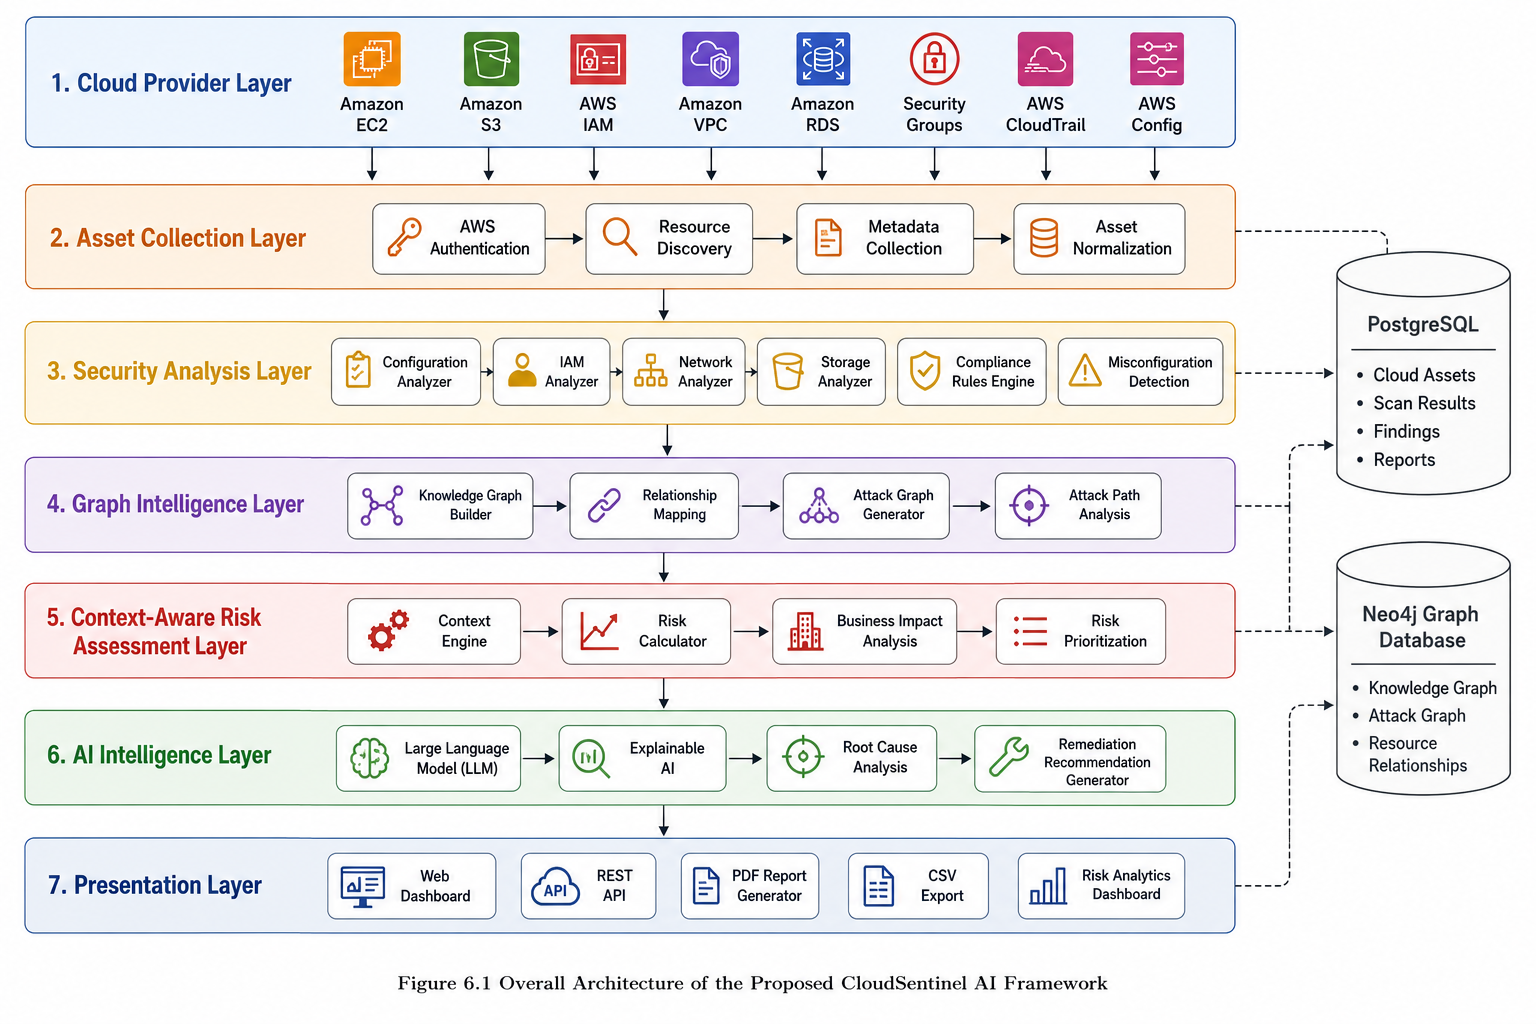
\includegraphics[width=0.9\textwidth,height=\textheight]{figures/image-6.1.png}
\caption{CloudSentinel AI System Architecture.}\label{fig:6_1}
}
\end{figure}

\subsection{6.2 Design Objectives}

The proposed framework has been designed with the following objectives:\\
\#\#\# 6.2.1 Automated Cloud Asset Discovery: The framework should automatically discover cloud resources by interacting with cloud provider APIs without requiring manual inventory creation. \#\#\# 6.2.2 Context-Aware Security Analysis: The framework should analyze relationships among identities, storage services, virtual machines, databases, networking components, and security policies to determine the overall security posture. \#\#\# 6.2.3 Attack Path Identification: The framework should identify possible attack paths by correlating multiple cloud misconfigurations. \#\#\# 6.2.4 Dynamic Risk Prioritization: Risk assessment should consider contextual information such as asset criticality, identity permissions, network exposure, and business impact instead of relying solely on predefined severity levels. \#\#\# 6.2.5 Explainable Security Recommendations: The framework should provide human-readable explanations describing detected security risks, possible attack scenarios, and recommended mitigation strategies. \#\#\# 6.2.6 Extensible System Design: The architecture should support future enhancements such as multi-cloud environments, Kubernetes security, Infrastructure-as-Code validation, and real-time security monitoring.

\subsection{6.3 Overall System Architecture}

CloudSentinel AI follows a modular architecture where each component performs a dedicated function while contributing to the overall security assessment process. The architecture consists of eight major modules that work together to transform raw cloud configuration data into actionable security intelligence. The overall workflow begins with cloud asset discovery, followed by configuration analysis, knowledge graph construction, attack path generation, context-aware risk engine processing, and explainable AI generation.

\subsection{6.4 Functional Modules of CloudSentinel AI}

\subsubsection{6.4.1 Cloud Asset Collector: Retrieves metadata regarding cloud resources directly from cloud provider APIs (e.g., AWS EC2, S3, IAM, VPC).}

\subsubsection{6.4.2 Configuration Analyzer: Evaluates resources against predefined security rules (e.g., public S3 buckets, overly permissive IAM, open security groups).}

\subsubsection{6.4.3 Knowledge Graph Builder: Transforms the cloud environment into an interconnected network, representing resources as nodes and relationships as edges.}

\subsubsection{6.4.4 Rule Engine: Evaluates cloud configurations using rules derived from CIS AWS Benchmarks, AWS Well-Architected Framework, and NIST guidelines.}

\subsubsection{6.4.5 Attack Graph Generator: Analyzes the knowledge graph to identify potential attack paths by correlating multiple cloud resources and security weaknesses.}

\subsubsection{6.4.6 Context-Aware Risk Engine: Calculates dynamic risk scores using factors like asset criticality, network exposure, and identity privileges.}

\subsubsection{6.4.7 Explainable AI Module: Generates human-readable explanations describing identified security issues, attack progression, and recommended remediation.}

\subsubsection{6.4.8 Dashboard and Reporting Module: Provides an interactive interface for visualizing security findings, attack paths, and risk scores.}

\subsection{6.5 Workflow of the Proposed Framework}

The operational workflow begins with cloud resource collection. Metadata is processed by the Configuration Analyzer and Rule Engine. The Knowledge Graph Builder then maps the environment, and the Attack Graph Generator identifies exploitation paths. These paths are evaluated by the Context-Aware Risk Engine, and the Explainable AI module provides remediation guidance through the Dashboard.

\subsection{6.6 Design Advantages of the Proposed Framework}

\begin{itemize}
\tightlist
\item
  Correlates cloud resources instead of analyzing them independently.\\
\item
  Generates attack paths representing realistic exploitation scenarios.\\
\item
  Utilizes graph-based reasoning for security assessment.\\
\item
  Performs contextual risk evaluation instead of static severity classification.\\
\item
  Provides Explainable AI-generated security recommendations.\\
\item
  Reduces alert fatigue by prioritizing exploitable attack chains.\\
\item
  Supports future extension to multi-cloud and cloud-native environments.
\end{itemize}

\subsection{6.7 Chapter Summary}

This chapter presented the CloudSentinel AI framework, detailing its modular architecture, design objectives, and operational workflow. By integrating graph-based modeling with AI-assisted security analysis, the proposed framework addresses the limitations identified in existing CSPM and CNAPP solutions. The next chapter details the research methodology, implementation strategy, and evaluation approach.

\subsection{Additional Figures}

\begin{figure}
\hypertarget{fig:6_2}{%
\centering
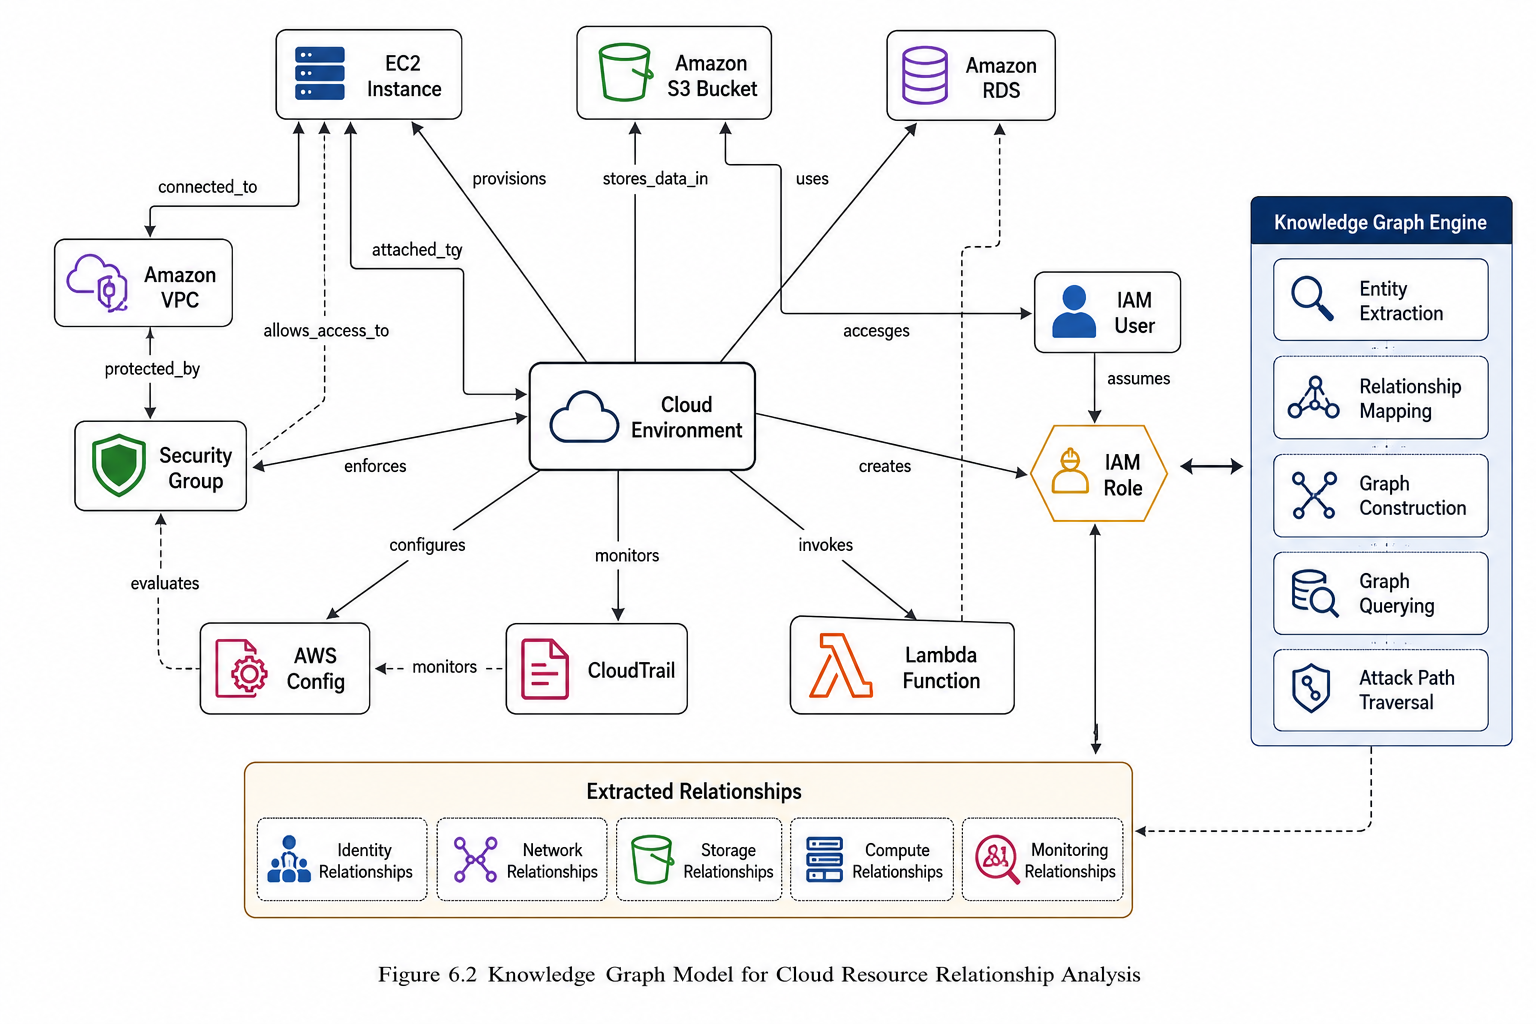
\includegraphics[width=0.9\textwidth,height=\textheight]{figures/image-6.2.png}
\caption{Cloud Asset and Security Analysis Workflow.}\label{fig:6_2}
}
\end{figure}

\begin{figure}
\hypertarget{fig:6_3}{%
\centering
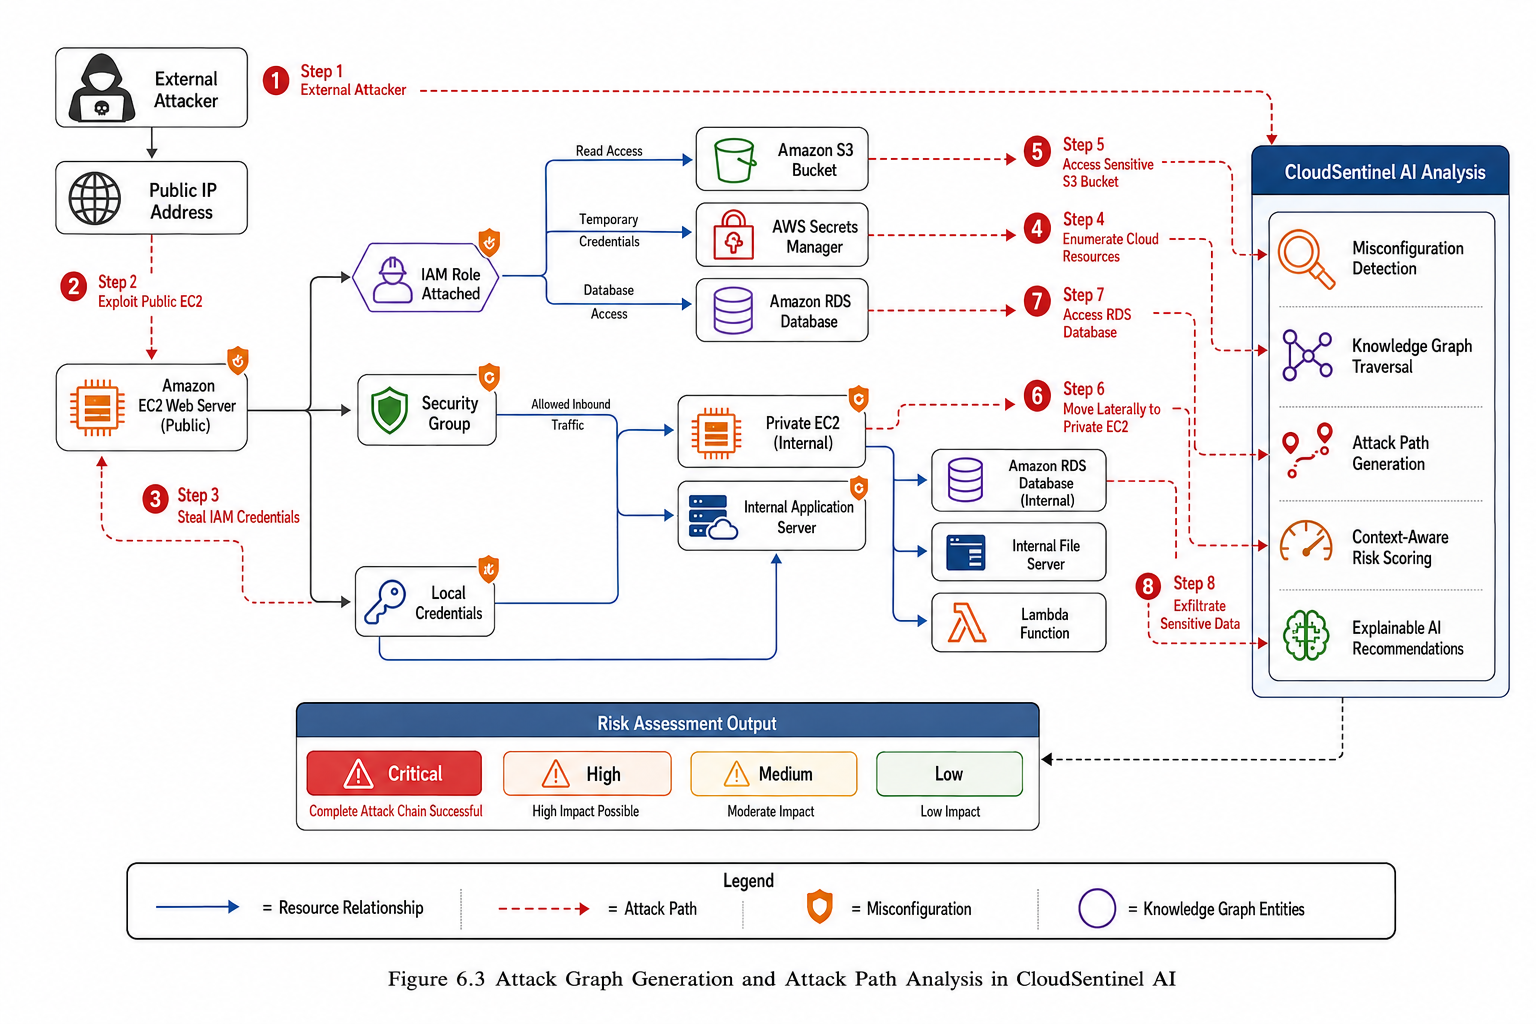
\includegraphics[width=0.9\textwidth,height=\textheight]{figures/image-6.3.png}
\caption{Knowledge Graph Construction Pipeline.}\label{fig:6_3}
}
\end{figure}

\begin{figure}
\hypertarget{fig:6_4}{%
\centering
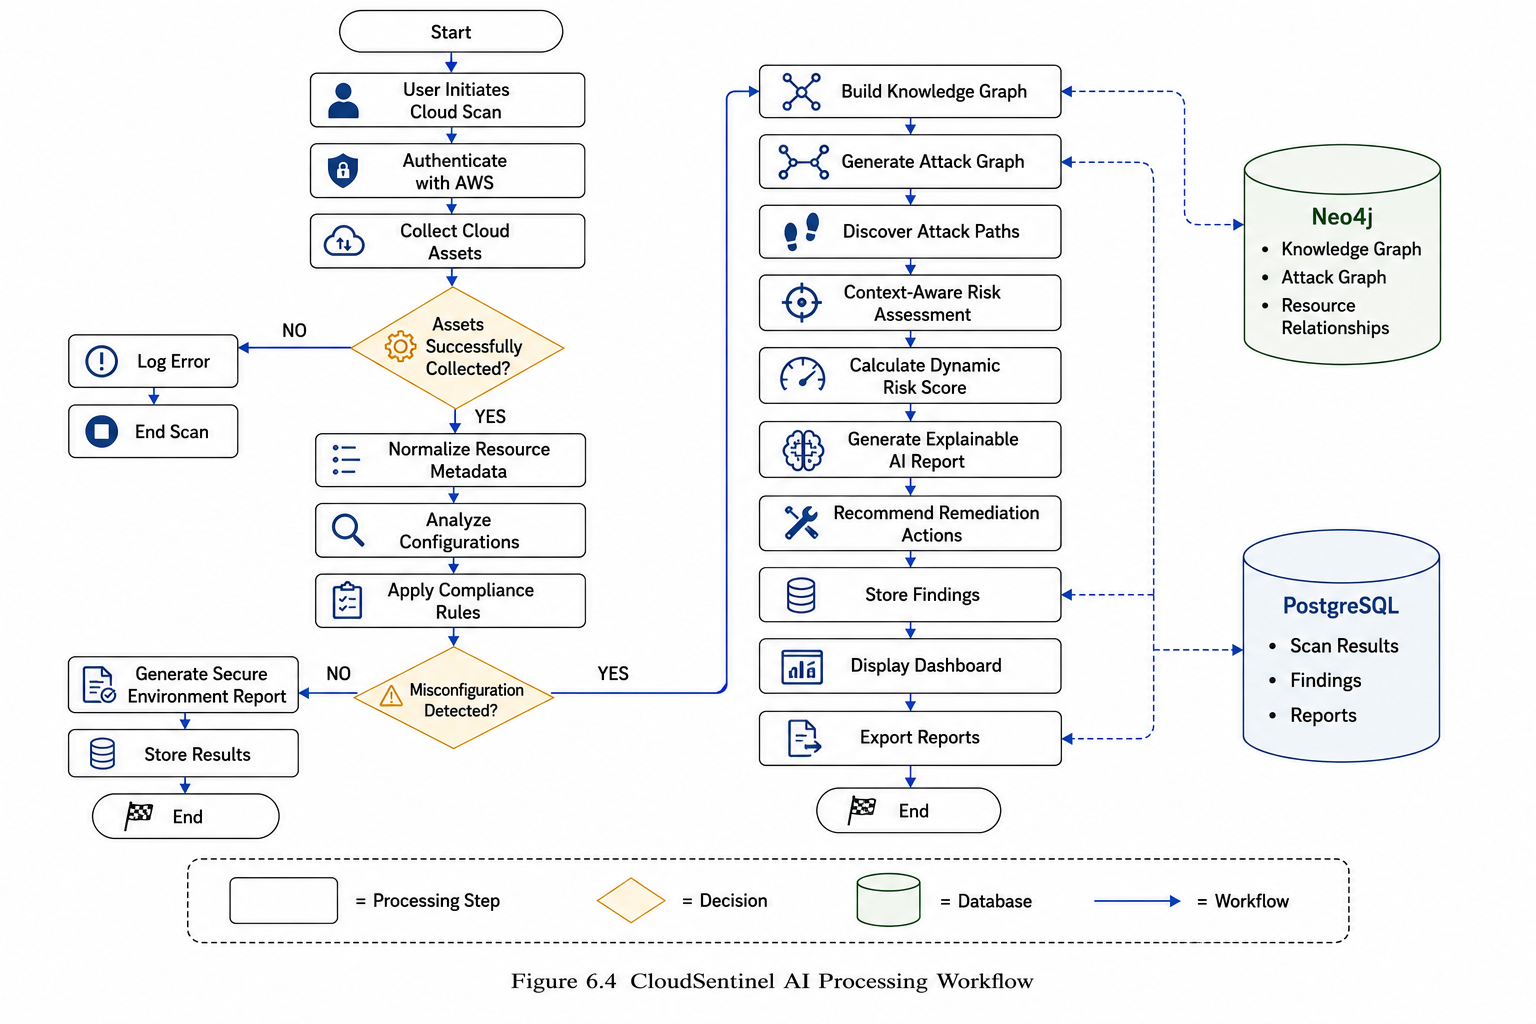
\includegraphics[width=0.9\textwidth,height=\textheight]{figures/image-6.4.png}
\caption{Context-Aware Risk Assessment Flow.}\label{fig:6_4}
}
\end{figure}

\section{Chapter 7 Research Methodology}

\subsection{7.1 Introduction}

This chapter presents the research methodology adopted for the design, development, and evaluation of the proposed CloudSentinel AI framework. The methodology provides a systematic approach for developing a context-aware cloud security solution capable of identifying cloud misconfigurations, modeling resource relationships, generating attack paths, assessing contextual risks, and producing explainable security recommendations. The proposed methodology combines cloud asset collection, graph-based data modeling, rule-based security assessment, contextual risk analysis, and Artificial Intelligence into a unified research framework. Each phase of the methodology builds upon the results of the previous phase, ensuring that the final system provides an accurate and comprehensive assessment of cloud security risks. The complete research methodology is illustrated in Figure 7.1, which depicts the sequential phases involved in the development and evaluation of CloudSentinel AI.

\begin{figure}[H]
\centering
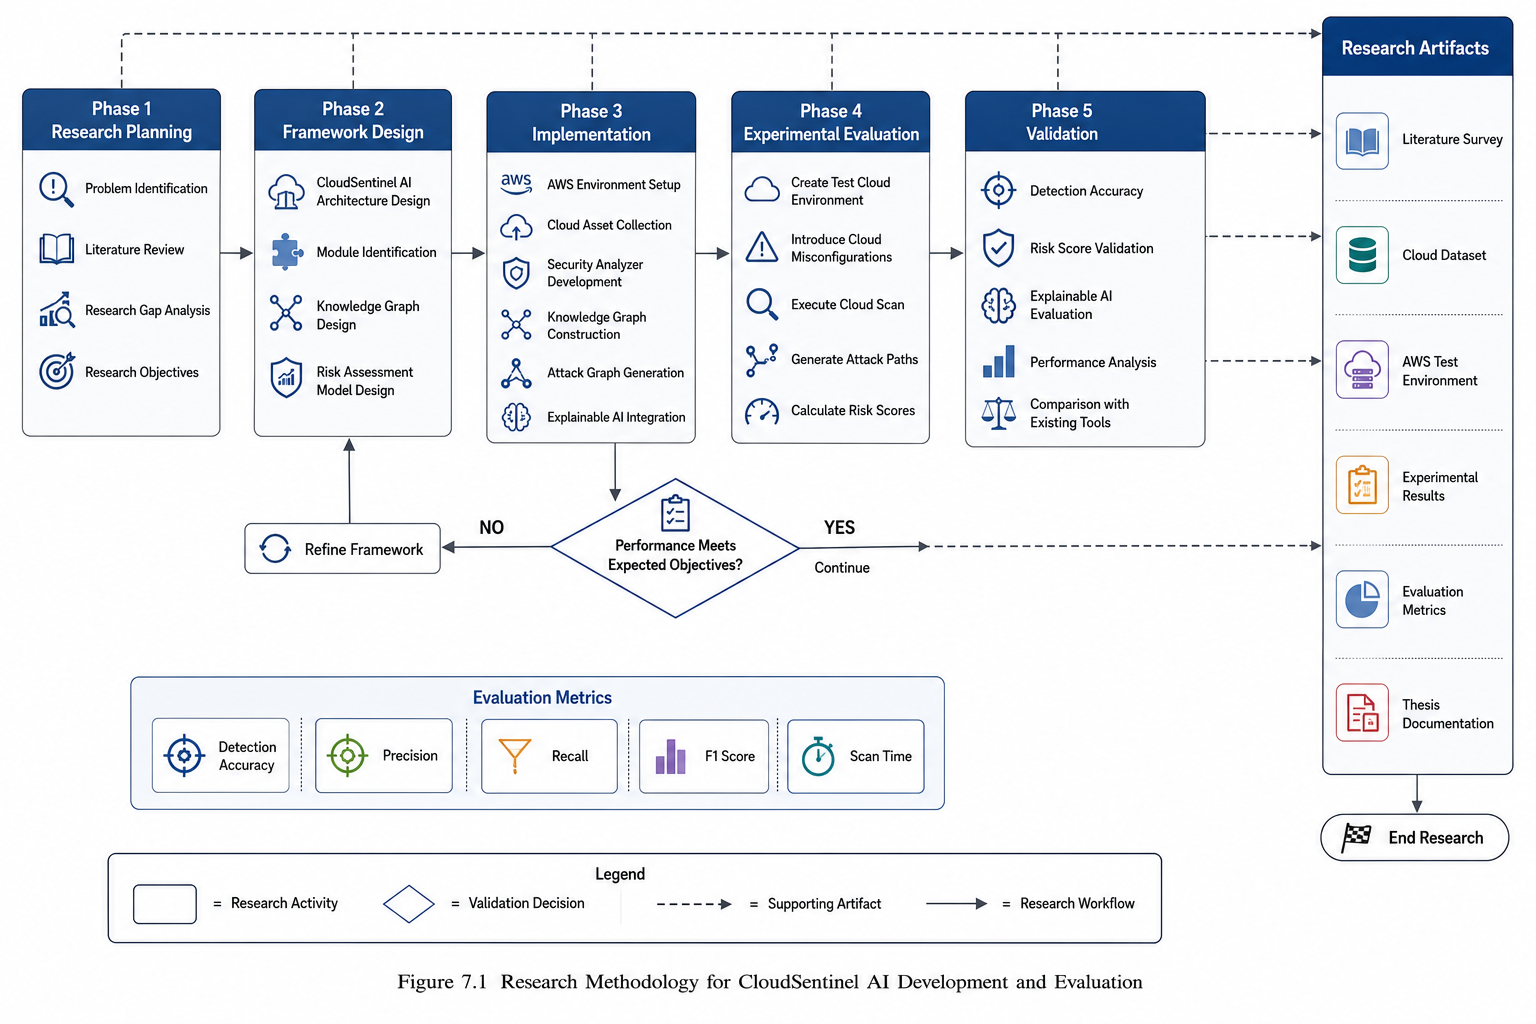
\includegraphics[width=0.9\textwidth,height=\textheight]{figures/image-7.1.png}
\caption{Research Methodology Workflow.}\label{fig:7_1}
\end{figure}

\subsection{7.2 Research Design}

The proposed research follows a Design Science Research (DSR) methodology \cite{hevner2004design}. Design Science Research is widely adopted in information systems and cybersecurity research because it focuses on creating and evaluating innovative artifacts that solve real-world problems. In this research, the primary artifact is the CloudSentinel AI framework, which is designed to address the limitations of existing Cloud Security Posture Management (CSPM) solutions. The research process consists of the following phases:

\begin{enumerate}
\def\labelenumi{\arabic{enumi}.}
\tightlist
\item
  Problem Identification\\
\item
  Requirement Analysis\\
\item
  Framework Design\\
\item
  System Development\\
\item
  Experimental Evaluation\\
\item
  Performance Analysis\\
\item
  Conclusion and Future Improvements
\end{enumerate}

Each phase contributes to the iterative refinement of the proposed framework, ensuring that the final solution addresses both practical cloud security challenges and the identified research gaps.

\subsection{7.3 Research Workflow}

The overall workflow of the proposed research consists of six major stages.\\
\textbf{Phase 1 -- Cloud Environment Preparation}\\
An AWS environment will be configured to simulate real-world cloud infrastructure. The environment will contain multiple AWS services, including EC2, IAM, S3, VPC, RDS, Security Groups, and CloudTrail. The cloud environment will intentionally include both secure and insecure configurations to evaluate the effectiveness of the proposed framework.\\
\textbf{Phase 2 -- Cloud Asset Collection}\\
The Cloud Asset Collector will communicate with AWS APIs to retrieve metadata describing cloud resources and their security configurations.\\
\textbf{Inputs:}

\begin{itemize}
\tightlist
\item
  AWS Credentials\\
\item
  AWS SDK (Boto3)\\
\item
  AWS Service APIs
\end{itemize}

\textbf{Processing:}

\begin{itemize}
\tightlist
\item
  Authenticate with AWS.\\
\item
  Discover cloud resources.\\
\item
  Retrieve metadata.\\
\item
  Store collected information.
\end{itemize}

\textbf{Outputs:}

\begin{itemize}
\tightlist
\item
  Cloud Asset Inventory\\
\item
  Configuration Metadata
\end{itemize}

\textbf{Phase 3 -- Configuration Assessment}\\
The collected cloud resources will be analyzed against predefined security policies derived from established cloud security frameworks.\\
\textbf{Inputs:}

\begin{itemize}
\tightlist
\item
  Cloud Resource Metadata\\
\item
  Security Policies\\
\item
  Compliance Rules
\end{itemize}

\textbf{Processing:}

\begin{itemize}
\tightlist
\item
  Evaluate configurations.\\
\item
  Detect policy violations.\\
\item
  Assign initial severity.
\end{itemize}

\textbf{Outputs:}

\begin{itemize}
\tightlist
\item
  Misconfiguration Report\\
\item
  Initial Security Findings
\end{itemize}

\textbf{Phase 4 -- Knowledge Graph Construction}\\
The validated cloud resources will be transformed into a graph representation.\\
\textbf{Inputs:}

\begin{itemize}
\tightlist
\item
  Cloud Resources\\
\item
  IAM Relationships\\
\item
  Network Topology\\
\item
  Storage Relationships
\end{itemize}

\textbf{Processing:}

\begin{itemize}
\tightlist
\item
  Create graph nodes.\\
\item
  Create graph edges.\\
\item
  Store graph.
\end{itemize}

\textbf{Outputs:}

\begin{itemize}
\tightlist
\item
  Knowledge Graph\\
\item
  Relationship Database
\end{itemize}

\textbf{Phase 5 -- Attack Path Generation}\\
The Knowledge Graph will be analyzed to identify realistic attack paths.\\
\textbf{Inputs:}

\begin{itemize}
\tightlist
\item
  Knowledge Graph
\end{itemize}

\textbf{Processing:}

\begin{itemize}
\tightlist
\item
  Traverse graph.\\
\item
  Identify exploitable paths.\\
\item
  Calculate attack chains.
\end{itemize}

\textbf{Outputs:}

\begin{itemize}
\tightlist
\item
  Attack Graph\\
\item
  Exploitation Paths
\end{itemize}

\textbf{Phase 6 -- Context-Aware Risk Assessment}\\
The identified attack paths will be evaluated using contextual information to generate dynamic risk scores.\\
\textbf{Inputs:}

\begin{itemize}
\tightlist
\item
  Attack Graph\\
\item
  Asset Criticality\\
\item
  Network Exposure\\
\item
  Identity Permissions
\end{itemize}

\textbf{Processing:}

\begin{itemize}
\tightlist
\item
  Analyze context.\\
\item
  Calculate dynamic risk.\\
\item
  Prioritize findings.
\end{itemize}

\textbf{Outputs:}

\begin{itemize}
\tightlist
\item
  Risk Score\\
\item
  Prioritized Findings
\end{itemize}

\textbf{Phase 7 -- Explainable AI Analysis}\\
The Explainable AI module converts technical findings into natural-language security recommendations.\\
\textbf{Inputs:}

\begin{itemize}
\tightlist
\item
  Attack Paths\\
\item
  Risk Scores
\end{itemize}

\textbf{Processing:}

\begin{itemize}
\tightlist
\item
  Generate explanation.\\
\item
  Produce remediation recommendations.
\end{itemize}

\textbf{Outputs:}

\begin{itemize}
\tightlist
\item
  Human-readable Security Report\\
\item
  AI Recommendations
\end{itemize}

\subsection{7.4 Research Environment}

The proposed framework will initially be developed and evaluated using Amazon Web Services (AWS).

\begin{itemize}
\tightlist
\item
  Cloud Platform: Amazon Web Services (AWS)\\
\item
  Programming Language: Python\\
\item
  Backend Framework: FastAPI\\
\item
  Graph Processing: NetworkX\\
\item
  Graph Database (Future Extension): Neo4j\\
\item
  Database: PostgreSQL\\
\item
  Dashboard: React.js\\
\item
  AI Integration: Large Language Model (LLM)\\
\item
  Version Control: Git and GitHub\\
\item
  Deployment: Docker
\end{itemize}

\subsection{7.5 Dataset}

Unlike traditional machine learning research, CloudSentinel AI does not rely on a static benchmark dataset. Instead, the framework generates its dataset dynamically by collecting metadata directly from cloud resources deployed within the AWS environment. The dataset consists of:

\begin{itemize}
\tightlist
\item
  IAM Policies\\
\item
  EC2 Configurations\\
\item
  Security Groups\\
\item
  VPC Configuration\\
\item
  S3 Bucket Policies\\
\item
  CloudTrail Logs\\
\item
  RDS Configuration\\
\item
  Encryption Settings
\end{itemize}

This approach ensures that the evaluation reflects realistic cloud environments rather than synthetic benchmark datasets.

\subsection{7.6 Evaluation Metrics}

The effectiveness of the proposed framework will be evaluated using multiple qualitative and quantitative metrics.\\
\textbf{Security Metrics:}

\begin{itemize}
\tightlist
\item
  Number of detected misconfigurations\\
\item
  Number of generated attack paths\\
\item
  Critical attack paths identified\\
\item
  False positive rate\\
\item
  False negative rate
\end{itemize}

\textbf{Performance Metrics:}

\begin{itemize}
\tightlist
\item
  Asset collection time\\
\item
  Graph construction time\\
\item
  Risk calculation time\\
\item
  Total assessment time
\end{itemize}

\textbf{AI Evaluation:}

\begin{itemize}
\tightlist
\item
  Explanation quality\\
\item
  Recommendation relevance\\
\item
  Analyst usability\\
\item
  Interpretability
\end{itemize}

\textbf{System Metrics:}

\begin{itemize}
\tightlist
\item
  CPU utilization\\
\item
  Memory usage\\
\item
  Scalability\\
\item
  API response time
\end{itemize}

\subsection{7.7 Research Validation}

To validate the effectiveness of CloudSentinel AI, the proposed framework will be compared against existing cloud security solutions. The comparison will focus on the following criteria:

\begin{itemize}
\tightlist
\item
  Cloud misconfiguration detection\\
\item
  Attack path identification\\
\item
  Context-aware risk analysis\\
\item
  Explainable AI support\\
\item
  Risk prioritization\\
\item
  Graph-based analysis\\
\item
  Analyst usability
\end{itemize}

Experimental results obtained from the proposed framework will be analyzed against these criteria to determine its effectiveness in improving cloud security assessment.

\subsection{7.8 Ethical Considerations}

All experiments conducted as part of this research will be performed within controlled cloud environments owned or authorized for research purposes. No unauthorized access to third-party cloud environments will be attempted. The framework is intended solely for defensive cybersecurity research, cloud security assessment, and educational purposes. The research complies with responsible disclosure principles and aims to improve cloud security practices without introducing risks to production systems.

\subsection{7.9 Chapter Summary}

This chapter presented the research methodology adopted for the development and evaluation of the proposed CloudSentinel AI framework. The methodology follows a structured Design Science Research approach, beginning with cloud environment preparation and progressing through cloud asset collection, configuration assessment, knowledge graph construction, attack path generation, contextual risk assessment, Explainable AI integration, and experimental validation. The methodology establishes a clear roadmap for implementing and evaluating the proposed framework while ensuring that each phase directly contributes to addressing the research gaps identified in earlier chapters.

\section{Chapter 8 System Design and Algorithmic Framework}

\subsection{8.1 Introduction}

This chapter presents the detailed system design and algorithmic framework of the proposed CloudSentinel AI system. While the previous chapter introduced the overall architecture and research methodology, this chapter focuses on the internal design of each module, the interaction among components, and the algorithms responsible for cloud security analysis. The proposed framework follows a modular architecture in which each component performs a dedicated function while exchanging structured information with other modules. This modular approach improves maintainability, scalability, and extensibility, allowing future integration with additional cloud providers and security services.

\subsection{8.2 Overall System Design}

CloudSentinel AI consists of eight interconnected modules that collectively perform cloud security assessment. The major modules are:

\begin{enumerate}
\def\labelenumi{\arabic{enumi}.}
\tightlist
\item
  Cloud Asset Collector\\
\item
  Configuration Analyzer\\
\item
  Knowledge Graph Builder\\
\item
  Rule Engine\\
\item
  Attack Graph Generator\\
\item
  Context-Aware Risk Engine\\
\item
  Explainable AI Module\\
\item
  Dashboard and Reporting Module
\end{enumerate}

The interaction between these modules follows a sequential pipeline in which the output of one module serves as the input for the next. This design minimizes coupling between components while enabling independent testing and future enhancements.

\subsection{8.3 Module Design}

\subsubsection{8.3.1 Cloud Asset Collector}

\textbf{Purpose:} The Cloud Asset Collector is responsible for discovering cloud resources and collecting metadata from the cloud environment. It provides the raw information required for all subsequent stages of security analysis.\\
\textbf{Inputs:} AWS Access Key, Secret Key, Session Token, Region, AWS SDK (Boto3).\\
\textbf{Processing:} Authenticates with AWS APIs and retrieves metadata. Normalizes collected data into a common internal format.\\
\textbf{Outputs:} Cloud Asset Inventory, Configuration Metadata, Resource Dependency Information.

\subsubsection{8.3.2 Configuration Analyzer}

\textbf{Purpose:} The Configuration Analyzer evaluates cloud resources against predefined security policies and compliance standards.\\
\textbf{Inputs:} Cloud Asset Inventory, Configuration Metadata, Security Policies.\\
\textbf{Processing:} Evaluates resources against rules (e.g., Public S3, Open Security Group). Assigns initial severity levels.\\
\textbf{Outputs:} Misconfiguration Report, Initial Severity Scores.

\subsubsection{8.3.3 Knowledge Graph Builder}

\textbf{Purpose:} The Knowledge Graph Builder models the cloud environment as a graph.\\
\textbf{Inputs:} Cloud Resources, IAM Relationships, Network Relationships, Resource Ownership.\\
\textbf{Processing:} Represents cloud resources as nodes and relationships as edges (e.g., IAM Role \(\rightarrow\) EC2).\\
\textbf{Outputs:} Knowledge Graph, Resource Relationship Graph.

\subsubsection{8.3.4 Rule Engine}

\textbf{Purpose:} Evaluate security rules and compliance requirements.\\
\textbf{Inputs:} Knowledge Graph, Security Policies.\\
\textbf{Processing:} Evaluates resources against frameworks like CIS AWS Benchmark, AWS Best Practices, NIST, and Organization Policies.\\
\textbf{Outputs:} Rule Violations, Compliance Report.

\subsubsection{8.3.5 Attack Graph Generator}

\textbf{Purpose:} Identify realistic attack paths across the cloud infrastructure.\\
\textbf{Inputs:} Knowledge Graph, Rule Violations.\\
\textbf{Processing:} Traverses the graph to identify connected resources that may be exploited sequentially (e.g., Internet \(\rightarrow\) EC2 \(\rightarrow\) IAM Role \(\rightarrow\) Secrets Manager \(\rightarrow\) S3).\\
\textbf{Outputs:} Attack Graph, Attack Chains, Reachability Report.

\subsubsection{8.3.6 Context-Aware Risk Engine}

\textbf{Purpose:} Calculate contextual risk scores.\\
\textbf{Inputs:} Attack Graph, Asset Criticality, Business Context, Network Exposure, Identity Privileges.\\
\textbf{Processing:} Evaluates factors like attack complexity, sensitive data, and network exposure to generate dynamic risk scores.\\
\textbf{Outputs:} Dynamic Risk Score, Prioritized Findings.

\subsubsection{8.3.7 Explainable AI Module}

\textbf{Purpose:} Generate human-readable security explanations.\\
\textbf{Inputs:} Risk Scores, Attack Graph, Rule Violations.\\
\textbf{Processing:} LLM interprets technical findings and generates reports including security issues, causes, attack scenarios, and remediation.\\
\textbf{Outputs:} AI Report, Remediation Suggestions.

\subsubsection{8.3.8 Dashboard and Reporting Module}

\textbf{Purpose:} Present findings to analysts.\\
\textbf{Inputs:} Risk Scores, Attack Graph, AI Report.\\
\textbf{Processing:} Organizes information into interactive views, including inventory, risk dashboard, and visualization.\\
\textbf{Outputs:} Interactive Dashboard, PDF Report.

\subsection{8.4 Algorithmic Framework}

The proposed framework employs several algorithms:

\subsubsection{8.4.1 Algorithm 1 -- Cloud Asset Collection}

\textbf{Objective:} Collect metadata from AWS services.\\
\textbf{Time Complexity:} O(n) where n is the number of resources.

\subsubsection{8.4.2 Algorithm 2 -- Knowledge Graph Construction}

\textbf{Objective:} Transform cloud resources into a graph.\\
\textbf{Time Complexity:} O(V + E) where V is resources and E is relationships.

\subsubsection{8.4.3 Algorithm 2 -- Attack Path Generation}

\textbf{Objective:} Generate possible attack paths.\\
\textbf{Time Complexity:} O(V + E) for graph traversal.

\subsubsection{8.4.4 Algorithm 4 -- Context-Aware Risk Scoring}

\textbf{Objective:} Calculate contextual risk.\\
\textbf{Time Complexity:} O(n) where n is the number of attack paths.

\subsubsection{8.4.5 Algorithm 5 -- Explainable AI Generation}

\textbf{Objective:} Generate human-readable explanations.\\
\textbf{Note:} Execution time depends on LLM latency.

\subsection{8.5 Chapter Summary}

This chapter presented the detailed system design and algorithmic framework of CloudSentinel AI. Each module was described in terms of its purpose, inputs, processing logic, outputs, and advantages. Additionally, the core algorithms responsible for asset collection, knowledge graph construction, attack path generation, contextual risk scoring, and Explainable AI were introduced. The modular architecture and algorithmic framework provide a clear technical blueprint for implementing the proposed system.

\subsection{Additional Figures}

\begin{figure}
\hypertarget{fig:8_1}{%
\centering
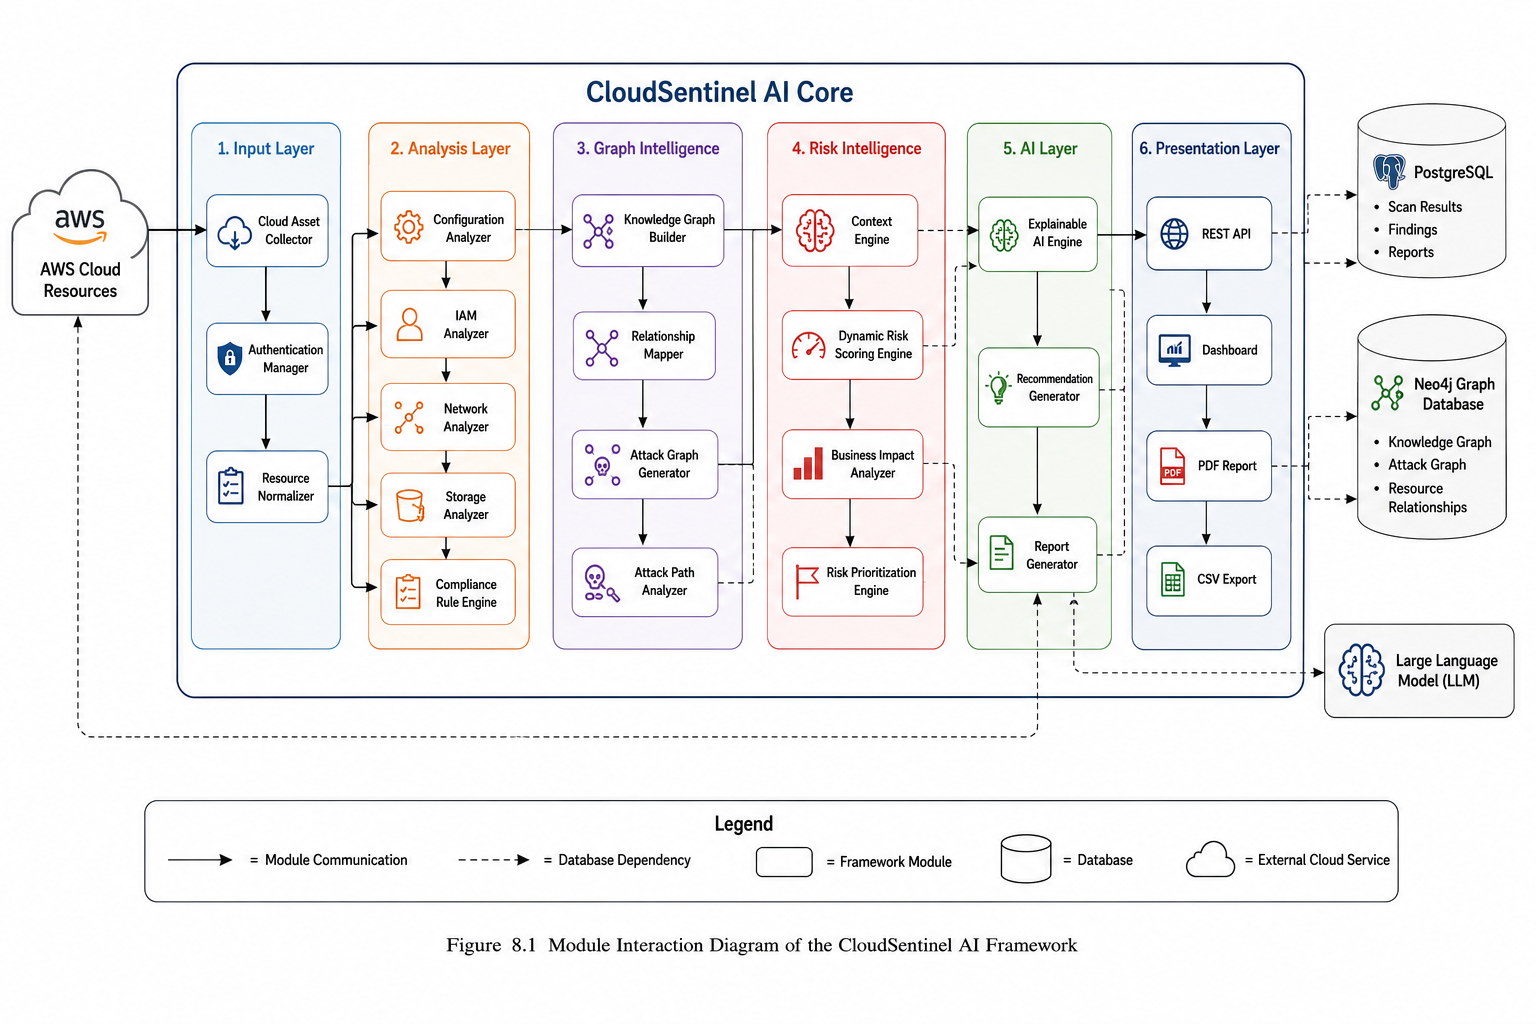
\includegraphics[width=0.9\textwidth,height=\textheight]{figures/image-8.1.png}
\caption{System Design and Algorithmic Framework.}\label{fig:8_1}
}
\end{figure}

\section{Chapter 9 Implementation and Technology Stack}

\subsection{9.1 Project Structure}

The CloudSentinel AI project is organized to ensure modularity, maintainability, and scalability. The project structure follows a standard software engineering pattern:

\begin{verbatim}
cloudsentinel-ai/
|-- backend/
|   |-- api/
|   |-- auth/
|   |-- collectors/
|   |-- analyzers/
|   |-- graph/
|   |-- attack_engine/
|   |-- risk_engine/
|   |-- ai/
|   |-- reports/
|   |-- database/
|-- frontend/
|   |-- dashboard/
|   |-- components/
|   |-- pages/
|   |-- services/
|-- infrastructure/
|   |-- docker/
|   |-- terraform/
|   |-- aws/
|-- docs/
|-- tests/
|-- README.md
\end{verbatim}

This structure clearly separates business logic, APIs, infrastructure, documentation, and testing, making the project easier to maintain and extend.

\subsection{9.2 Backend Technology Stack}

The backend of CloudSentinel AI is developed using Python, leveraging the FastAPI framework. FastAPI was selected for its high performance, native support for asynchronous programming, and automated data validation features. It provides an efficient platform for handling high-concurrency requests, which is essential for scanning large cloud environments and processing complex graph-based queries.

\subsection{9.3 Frontend Development}

The frontend is built using React.js to provide a responsive, intuitive interface for security analysts. To handle the complex visualization of cloud attack graphs, the dashboard integrates specialized libraries such as Cytoscape.js or D3.js. These tools enable the rendering of interactive nodes and edges, allowing users to zoom, pan, and filter attack paths dynamically.

\subsection{9.4 Database and Data Modeling}

The framework employs a hybrid data storage strategy:

\begin{itemize}
\tightlist
\item
  \textbf{PostgreSQL:} Serves as the primary relational database for storing persistent configuration data, user information, audit logs, and scan history.\\
\item
  \textbf{NetworkX:} Used for in-memory graph construction and algorithm execution during analysis.\\
\item
  \textbf{Graph Database (Future):} While currently utilizing in-memory structures for agility, the architecture is designed to integrate graph-native databases like Neo4j or Amazon Neptune as the environment scale increases.
\end{itemize}

\subsection{9.5 AI and LLM Integration}

The Explainable AI module integrates with Large Language Models (LLMs) through secure API interfaces. The backend processes raw graph data and rule violations, structures them into a context-rich prompt, and sends them to the LLM. The model is specifically tuned through prompt engineering to return standardized, actionable security reports, minimizing hallucinations and ensuring technical accuracy.

\subsection{9.6 Infrastructure and DevOps}

Infrastructure is managed using containerization and Infrastructure-as-Code (IaC) principles:

\begin{itemize}
\tightlist
\item
  \textbf{Docker:} Ensures consistent deployment environments across development, staging, and production by bundling all dependencies.\\
\item
  \textbf{Terraform:} Facilitates the automated provisioning of the infrastructure stack, ensuring scalability, environmental reproducibility, and consistent management of cloud resources.
\end{itemize}

\subsection{9.7 API Design and Documentation}

The application follows RESTful API design principles to ensure a clean interface between the backend engines and the frontend dashboard. All endpoints are secured with JSON Web Token (JWT) authentication, ensuring that only authorized users can trigger scans or view sensitive security findings. The API is documented using the OpenAPI (Swagger) specification, providing clear endpoint definitions and enabling seamless integration for future development.

\subsection{9.8 Security Considerations}

To ensure secure operation, the implementation incorporates several security measures:

\begin{itemize}
\tightlist
\item
  \textbf{Secure Credential Storage:} Utilization of IAM roles or AWS Secrets Manager to manage sensitive credentials.\\
\item
  \textbf{Encrypted Communication:} Enforcement of HTTPS for all client-server communication.\\
\item
  \textbf{Access Control:} Implementation of Role-Based Access Control (RBAC) for all dashboard users.\\
\item
  \textbf{Cryptographic Security:} Password hashing using secure cryptographic algorithms.\\
\item
  \textbf{Auditability:} Comprehensive audit logging for all scan operations.\\
\item
  \textbf{Input Sanitization:} Strict input validation and API request sanitization to prevent injection attacks.\\
\item
  \textbf{Traffic Control:} Rate limiting applied to public endpoints to mitigate denial-of-service risks.\\
\item
  \textbf{Data Protection:} Secure handling of AI-generated reports to prevent sensitive data leakage.
\end{itemize}

\subsection{9.9 Scalability and Future Enhancements}

The modular implementation enables future expansion without significant architectural changes. Potential enhancements include:

\begin{itemize}
\tightlist
\item
  \textbf{Multi-Cloud Support:} Extending coverage to Azure and GCP.\\
\item
  \textbf{Kubernetes Security:} Integration of container and orchestration-level security analysis.\\
\item
  \textbf{IaC Scanning:} Automated security validation for Infrastructure-as-Code templates.\\
\item
  \textbf{Real-time Monitoring:} Implementation of event-driven monitoring using cloud-native triggers.\\
\item
  \textbf{Compliance Automation:} Continuous, automated compliance assessment frameworks.\\
\item
  \textbf{SIEM Integration:} Data export capabilities for Security Information and Event Management platforms.\\
\item
  \textbf{Automated Remediation:} Development of guided or automated remediation workflows.
\end{itemize}

\subsection{9.10 Chapter Summary}

This chapter described the implementation design and technology stack of CloudSentinel AI. It explained the rationale behind the selected technologies, the deployment architecture, the hybrid relational and graph data model, the REST API design, the project structure, and the security considerations that guide the implementation. The proposed implementation emphasizes modularity, scalability, and maintainability while providing a practical roadmap for developing the CloudSentinel AI framework.

\subsection{Additional Figures}

\begin{figure}[H]
\centering
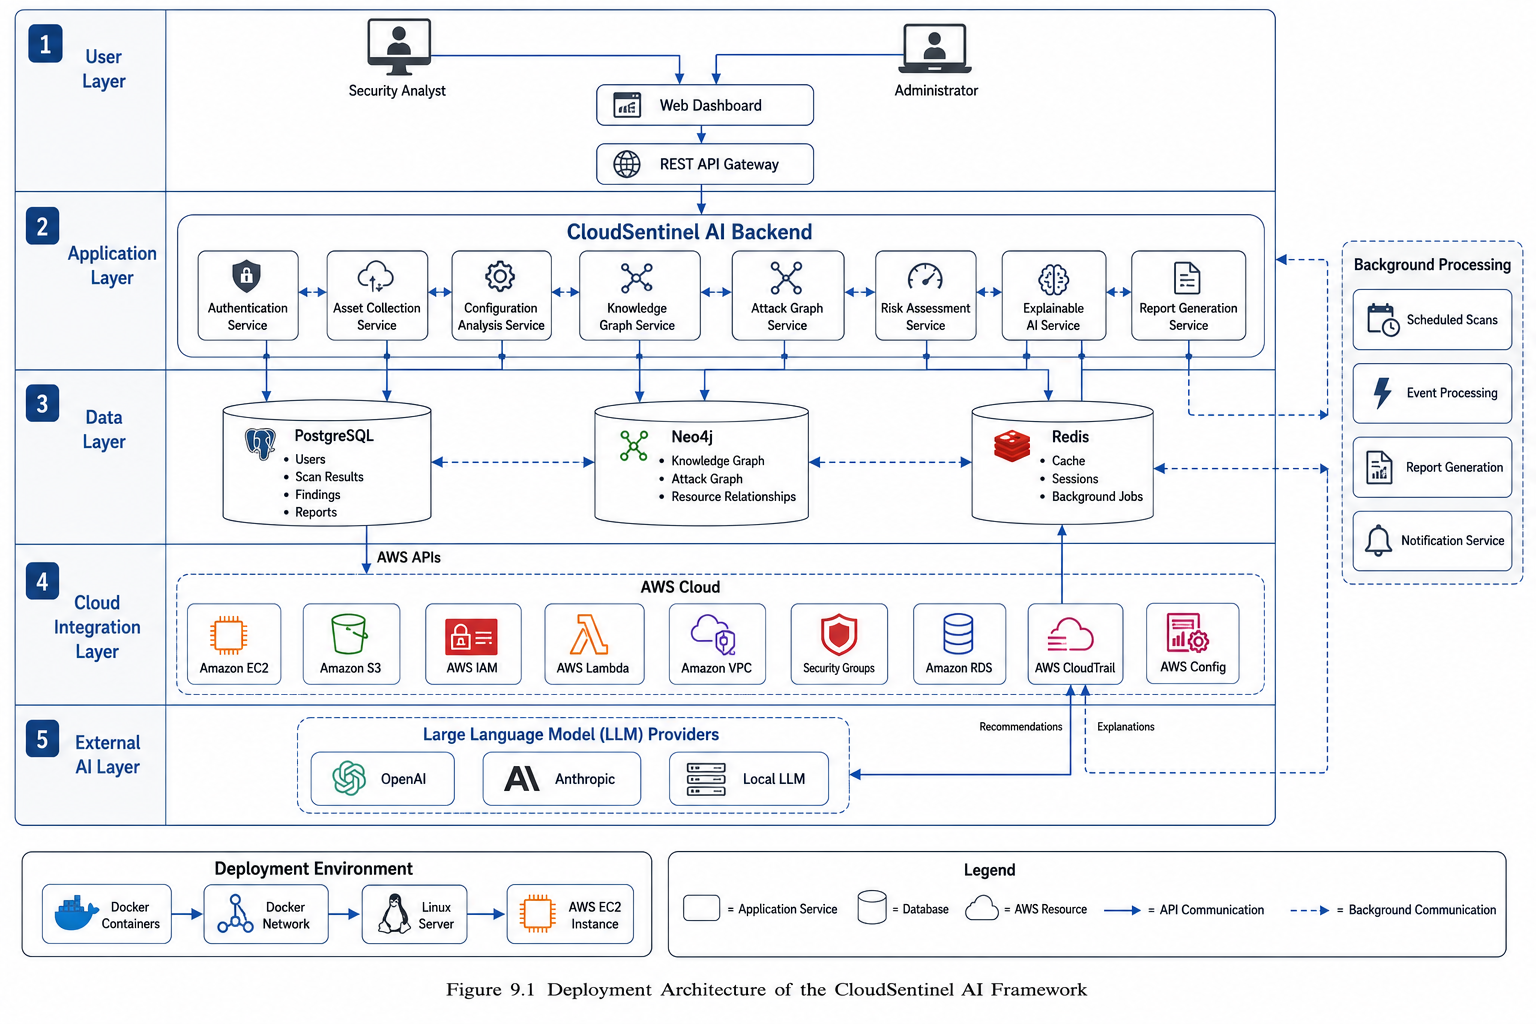
\includegraphics[width=0.9\textwidth,height=\textheight]{figures/image-9.1.png}
\caption{Knowledge Graph Representation.}\label{fig:9_1}
\end{figure}

\begin{figure}[H]
\centering
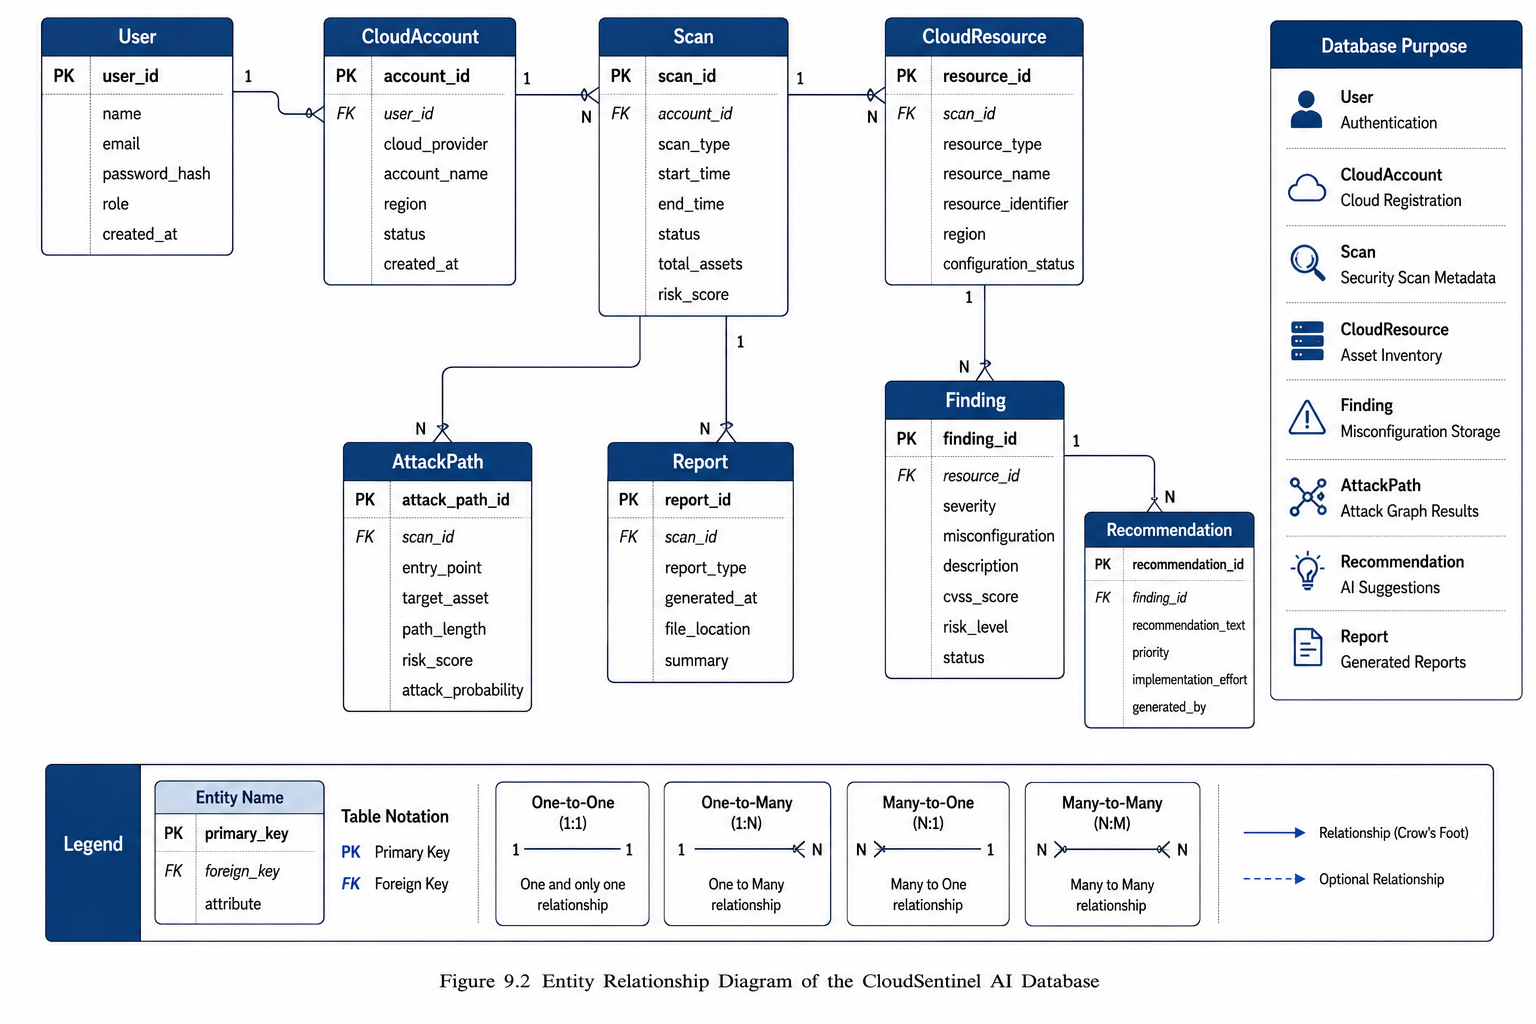
\includegraphics[width=0.9\textwidth,height=\textheight]{figures/image-9.2.png}
\caption{Attack Graph Generation Process.}\label{fig:9_2}
\end{figure}

\begin{figure}[H]
\centering
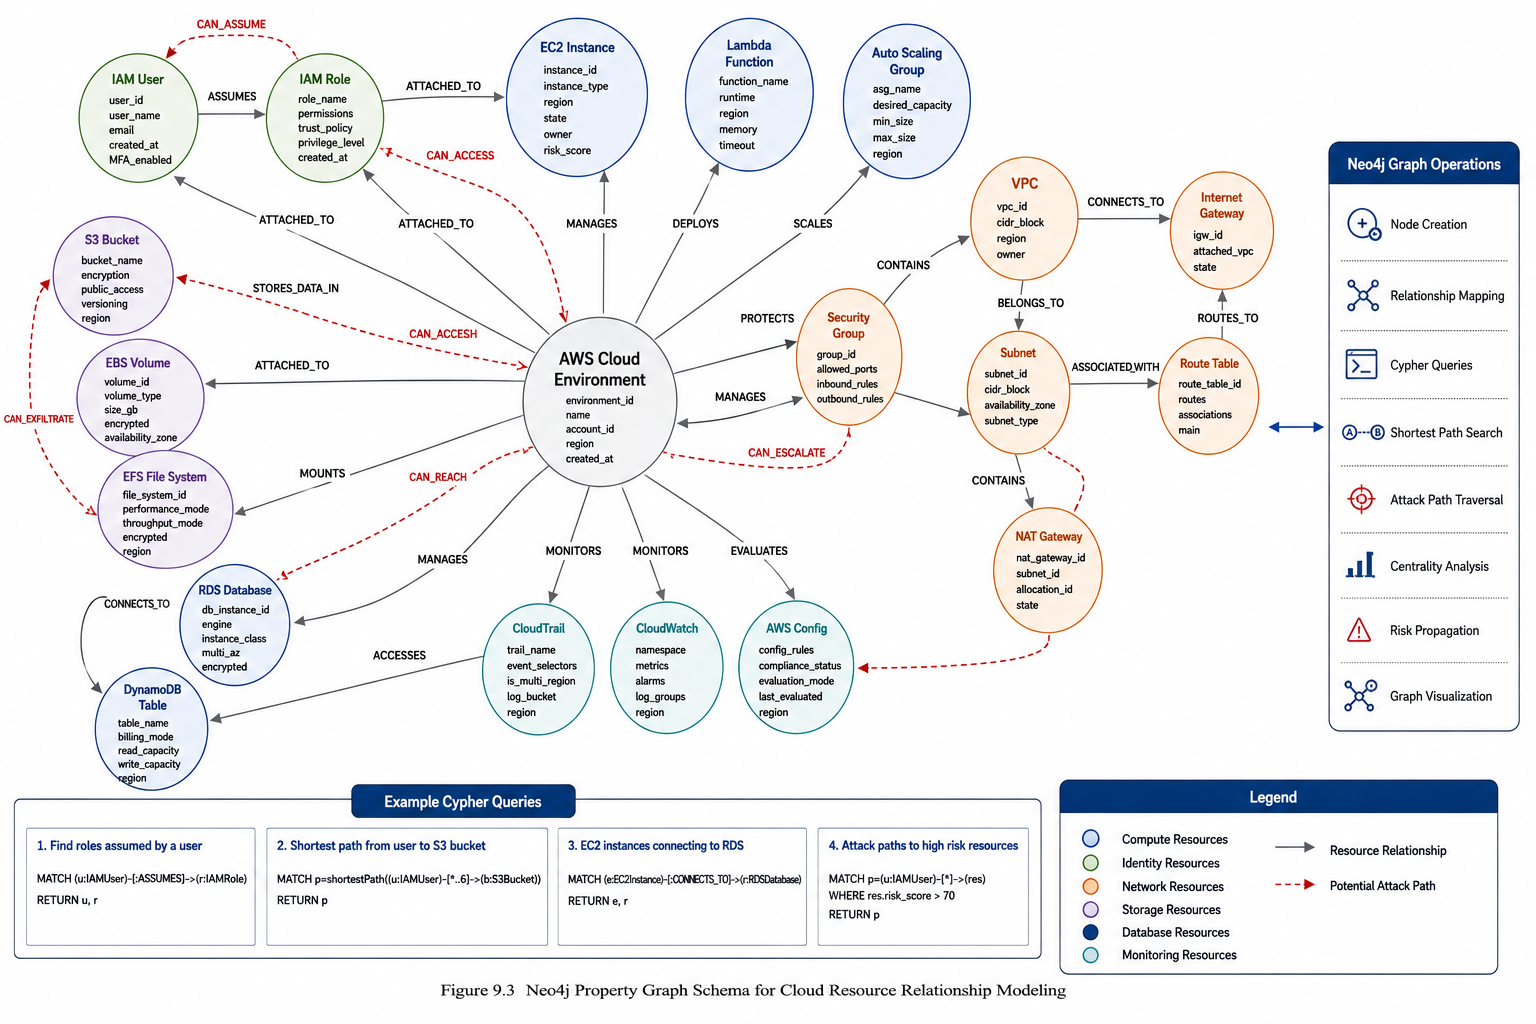
\includegraphics[width=0.9\textwidth,height=\textheight]{figures/image-9.3.png}
\caption{Context-Aware Risk Prioritization.}\label{fig:9_3}
\end{figure}

\section{Chapter 10 Experimental Design and Evaluation Plan}

\subsection{10.1 Introduction}

This chapter presents the experimental design and evaluation methodology proposed for validating the effectiveness of the CloudSentinel AI framework. The objective of the experimental evaluation is to determine whether the proposed framework improves cloud security assessment when compared with existing Cloud Security Posture Management (CSPM) solutions. The evaluation focuses on four key aspects:

\begin{itemize}
\tightlist
\item
  Accuracy of cloud misconfiguration detection\\
\item
  Identification of multi-stage attack paths\\
\item
  Effectiveness of context-aware risk prioritization\\
\item
  Quality and usefulness of AI-generated security explanations
\end{itemize}

The overall evaluation workflow is illustrated in Figure 10.1, showing the sequence from cloud environment preparation to comparative analysis.

\begin{figure}[H]
\centering
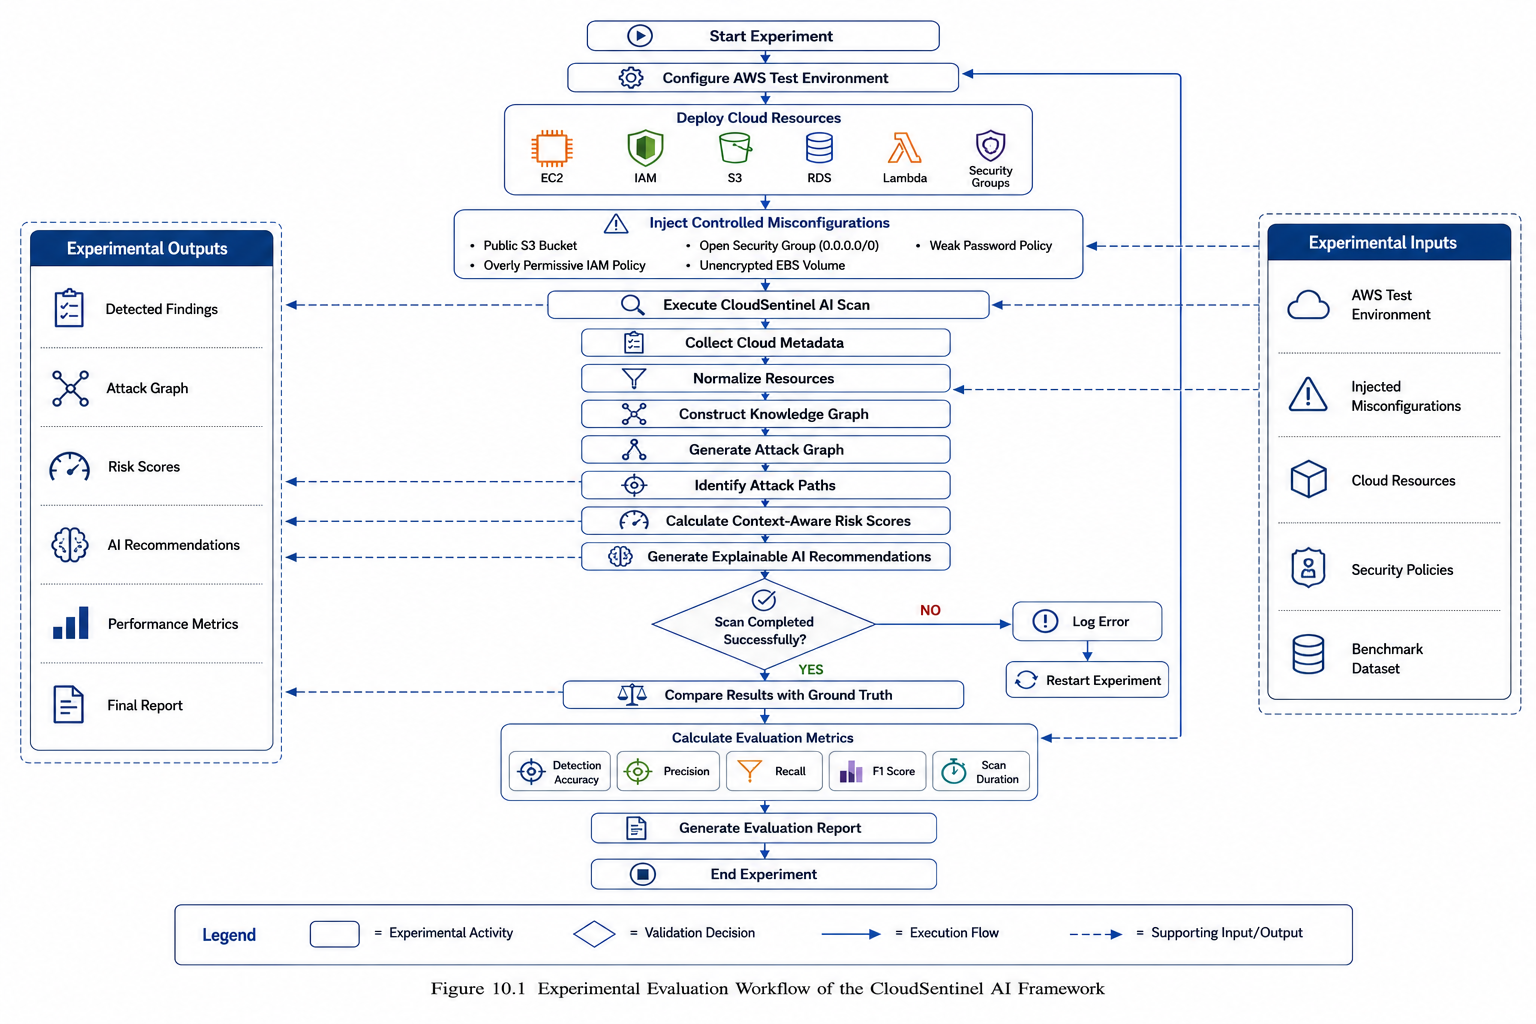
\includegraphics[width=0.9\textwidth,height=\textheight]{figures/image-10.1.png}
\caption{Experimental Evaluation Workflow.}\label{fig:10_1}
\end{figure}

\subsection{10.2 Experimental Objectives}

The experiments are designed to evaluate the proposed framework against predefined research objectives.

\begin{itemize}
\tightlist
\item
  \textbf{Objective 1:} Evaluate the ability of CloudSentinel AI to identify cloud misconfigurations across AWS resources.\\
\item
  \textbf{Objective 2:} Measure the framework's capability to generate realistic attack paths by correlating multiple cloud resources.\\
\item
  \textbf{Objective 3:} Assess the effectiveness of contextual risk scoring compared to static severity classifications.\\
\item
  \textbf{Objective 4:} Evaluate the quality and interpretability of AI-generated security explanations.\\
\item
  \textbf{Objective 5:} Compare the overall performance of CloudSentinel AI with selected baseline cloud security tools.
\end{itemize}

\subsection{10.3 Experimental Environment}

All experiments will be conducted in a controlled Amazon Web Services (AWS) environment to ensure reproducibility and minimize external influences.

\begin{longtable}[]{@{}ll@{}}
\toprule\noalign{}
Component & Specification \\
\midrule\noalign{}
\endhead
\bottomrule\noalign{}
\endlastfoot
Cloud Platform & Amazon Web Services (AWS) \\
Operating System & Ubuntu Linux \\
Programming Language & Python \\
Backend Framework & FastAPI \\
Graph Library & NetworkX \\
Database & PostgreSQL \\
Container Platform & Docker \\
Version Control & GitHub \\
\end{longtable}

\subsection{10.4 Experimental Scenarios}

To evaluate the framework under realistic conditions, several cloud environments with intentionally introduced security weaknesses will be created.

\begin{itemize}
\tightlist
\item
  \textbf{Scenario 1 -- Public Storage Exposure:} Amazon S3 buckets will be configured with public read or write permissions. Expected Outcome: Detect public bucket, sensitive data exposure, business impact, and remediation recommendation.\\
\item
  \textbf{Scenario 2 -- Overly Permissive IAM Policies:} IAM users and roles will be assigned excessive administrative privileges. Expected Outcome: Identify privilege escalation risks, excessive permissions, and potential attack paths.\\
\item
  \textbf{Scenario 3 -- Insecure Network Configuration:} Security Groups will intentionally expose SSH and RDP ports to the Internet. Expected Outcome: Detect internet-facing resources, network exposure, and possible attack chains.\\
\item
  \textbf{Scenario 4 -- Disabled Logging:} AWS CloudTrail logging will be disabled. Expected Outcome: Identify reduced visibility, explain the impact on forensic investigations, and recommend enabling centralized logging.\\
\item
  \textbf{Scenario 5 -- Multi-Stage Attack Chain:} A realistic attack chain will be constructed by combining a public EC2 instance, weak Security Group, excessive IAM permissions, access to AWS Secrets Manager, and sensitive S3 bucket. Expected Outcome: Generate a complete attack graph demonstrating how an attacker could move from the exposed EC2 instance to sensitive data.
\end{itemize}

\subsection{10.5 Baseline Tools for Comparison}

To evaluate the effectiveness of CloudSentinel AI, the experimental results will be compared with established cloud security tools.

\begin{longtable}[]{@{}
  >{\raggedright\arraybackslash}p{(\columnwidth - 8\tabcolsep) * \real{0.2000}}
  >{\raggedright\arraybackslash}p{(\columnwidth - 8\tabcolsep) * \real{0.2000}}
  >{\raggedright\arraybackslash}p{(\columnwidth - 8\tabcolsep) * \real{0.2000}}
  >{\raggedright\arraybackslash}p{(\columnwidth - 8\tabcolsep) * \real{0.2000}}
  >{\raggedright\arraybackslash}p{(\columnwidth - 8\tabcolsep) * \real{0.2000}}@{}}
\toprule\noalign{}
\begin{minipage}[b]{\linewidth}\raggedright
Tool
\end{minipage} & \begin{minipage}[b]{\linewidth}\raggedright
Misconfiguration Detection
\end{minipage} & \begin{minipage}[b]{\linewidth}\raggedright
Attack Path Analysis
\end{minipage} & \begin{minipage}[b]{\linewidth}\raggedright
Context-Aware Risk
\end{minipage} & \begin{minipage}[b]{\linewidth}\raggedright
Explainable AI
\end{minipage} \\
\midrule\noalign{}
\endhead
\bottomrule\noalign{}
\endlastfoot
AWS Security Hub & \(\checkmark\) & \(\times\) & Limited & \(\times\) \\
AWS Config & \(\checkmark\) & \(\times\) & \(\times\) & \(\times\) \\
Prowler & \(\checkmark\) & \(\times\) & \(\times\) & \(\times\) \\
ScoutSuite & \(\checkmark\) & Partial & \(\times\) & \(\times\) \\
CloudSentinel AI & \(\checkmark\) & \(\checkmark\) & \(\checkmark\) & \(\checkmark\) \\
\end{longtable}

\subsection{10.6 Evaluation Metrics}

The performance of CloudSentinel AI will be assessed using quantitative and qualitative evaluation metrics.

\subsubsection{10.6.1 Detection Metrics}

\begin{itemize}
\tightlist
\item
  Number of discovered resources\\
\item
  Number of detected misconfigurations\\
\item
  Detection coverage\\
\item
  False Positive Rate (FPR)\\
\item
  False Negative Rate (FNR)
\end{itemize}

\subsubsection{10.6.2 Performance Metrics}

\begin{itemize}
\tightlist
\item
  Asset discovery time\\
\item
  Configuration analysis time\\
\item
  Knowledge graph construction time\\
\item
  Attack graph generation time\\
\item
  Context-aware risk assessment time\\
\item
  Total execution time\\
\item
  CPU utilization\\
\item
  Memory consumption
\end{itemize}

\subsubsection{10.6.3 Attack Path Metrics}

\begin{itemize}
\tightlist
\item
  Number of generated attack paths\\
\item
  Average attack path length\\
\item
  Reachability between critical assets\\
\item
  Critical attack chains identified
\end{itemize}

\subsubsection{10.6.4 Risk Prioritization Metrics}

\begin{itemize}
\tightlist
\item
  Accuracy of prioritization\\
\item
  High-risk asset identification\\
\item
  Reduction in low-value alerts\\
\item
  Consistency of contextual scoring
\end{itemize}

\subsubsection{10.6.5 Explainable AI Metrics}

\begin{itemize}
\tightlist
\item
  Clarity of explanations\\
\item
  Completeness of recommendations\\
\item
  Technical accuracy\\
\item
  Readability for security analysts\\
\item
  Actionability of remediation guidance
\end{itemize}

\subsection{10.7 Experimental Workflow}

\begin{enumerate}
\def\labelenumi{\arabic{enumi}.}
\tightlist
\item
  Deploy the AWS test environment with predefined configurations.\\
\item
  Introduce controlled cloud misconfigurations for each experimental scenario.\\
\item
  Execute CloudSentinel AI to collect cloud assets and identify security issues.\\
\item
  Construct the knowledge graph representing cloud resources and their relationships.\\
\item
  Generate attack paths based on graph traversal and detected vulnerabilities.\\
\item
  Calculate contextual risk scores for each attack path.\\
\item
  Generate AI-assisted explanations and remediation recommendations.\\
\item
  Execute baseline tools under identical conditions.\\
\item
  Compare results using the selected evaluation metrics.\\
\item
  Analyze the findings and summarize the performance of the proposed framework.
\end{enumerate}

\subsection{10.8 Data Analysis Strategy}

The collected experimental data will be analyzed using descriptive statistics and comparative analysis. This includes comparison of detection rates, attack path identification, contextual risk prioritization effectiveness, execution times, and usefulness of AI-generated explanations.

\subsection{10.9 Threats to Validity}

\begin{itemize}
\tightlist
\item
  \textbf{Internal Validity:} Test environments may not represent every real-world AWS deployment.\\
\item
  \textbf{External Validity:} The initial implementation focuses on AWS; results may differ for Azure, Google Cloud Platform, or hybrid environments.\\
\item
  \textbf{Construct Validity:} Risk scores depend on the contextual factors selected for evaluation.\\
\item
  \textbf{Conclusion Validity:} Performance measurements may vary with hardware specifications, cloud environment size, and network conditions.
\end{itemize}

\subsection{10.10 Expected Outcomes}

CloudSentinel AI is expected to detect misconfigurations with high accuracy, generate meaningful multi-stage attack paths, prioritize risks effectively, reduce alert fatigue, and provide clear, actionable AI-generated explanations.

\subsection{10.11 Chapter Summary}

This chapter presented the experimental design and evaluation plan for validating the CloudSentinel AI framework. It defined the objectives, environment, scenarios, baseline tools, metrics, workflow, data analysis strategy, and threats to validity, establishing a structured approach for validating the research.

\subsection{Additional Figures}

\begin{figure}[H]
\centering
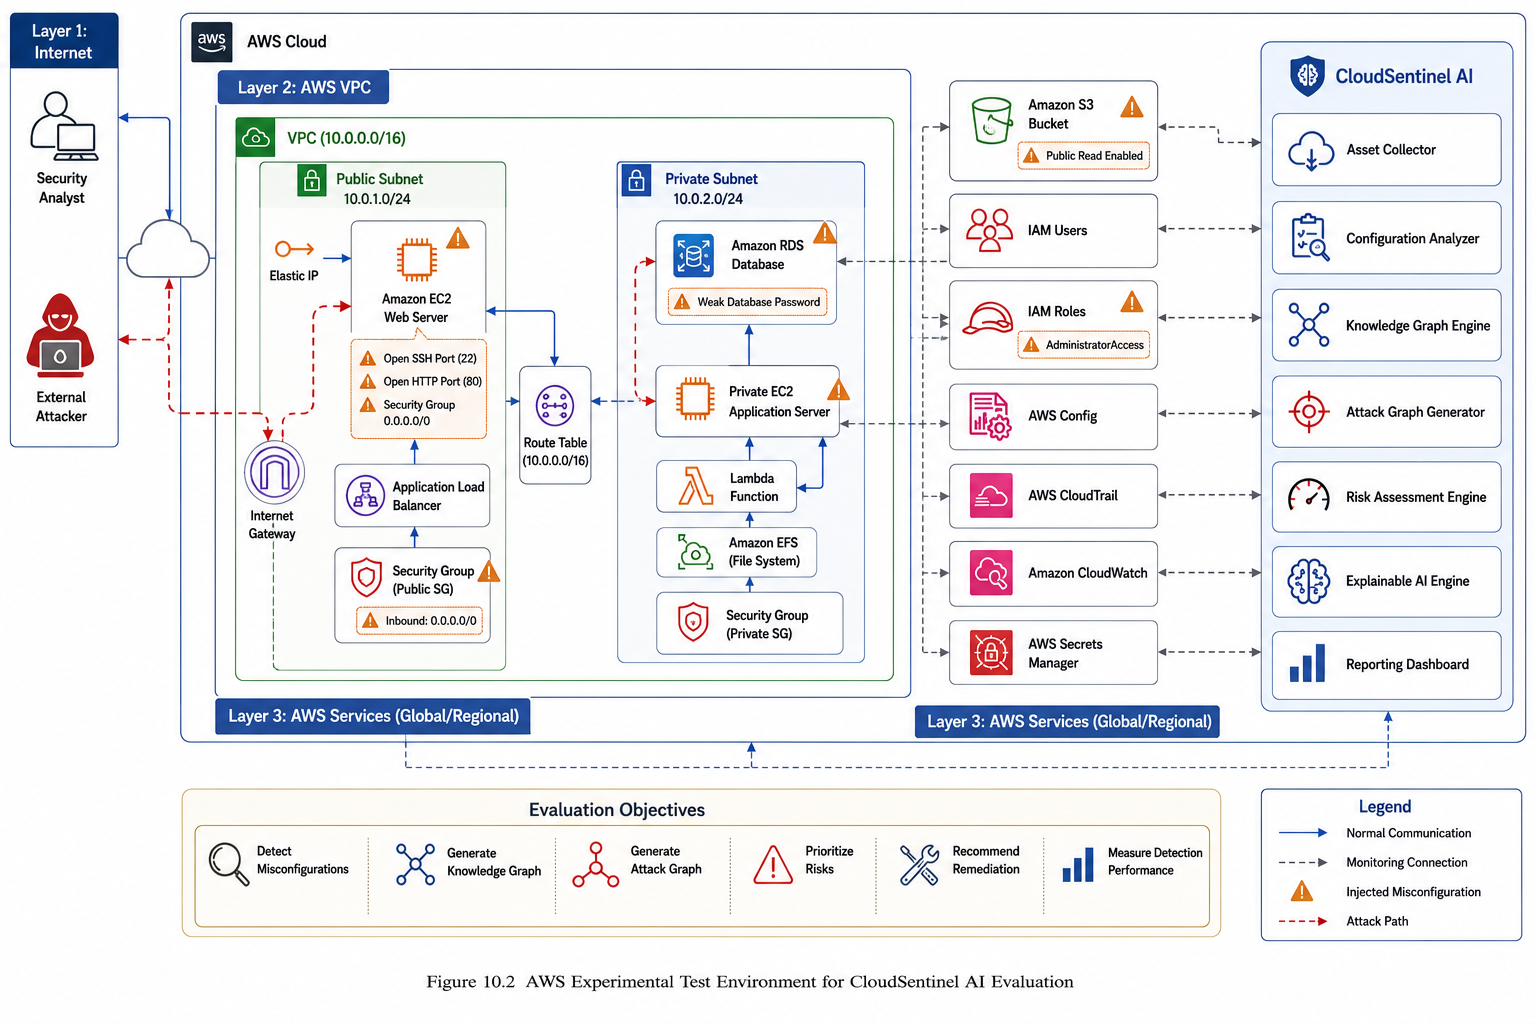
\includegraphics[width=0.9\textwidth,height=\textheight]{figures/image-10.2.png}
\caption{Injected Misconfiguration Scenario Design.}\label{fig:10_2}
\end{figure}

\begin{figure}[H]
\centering
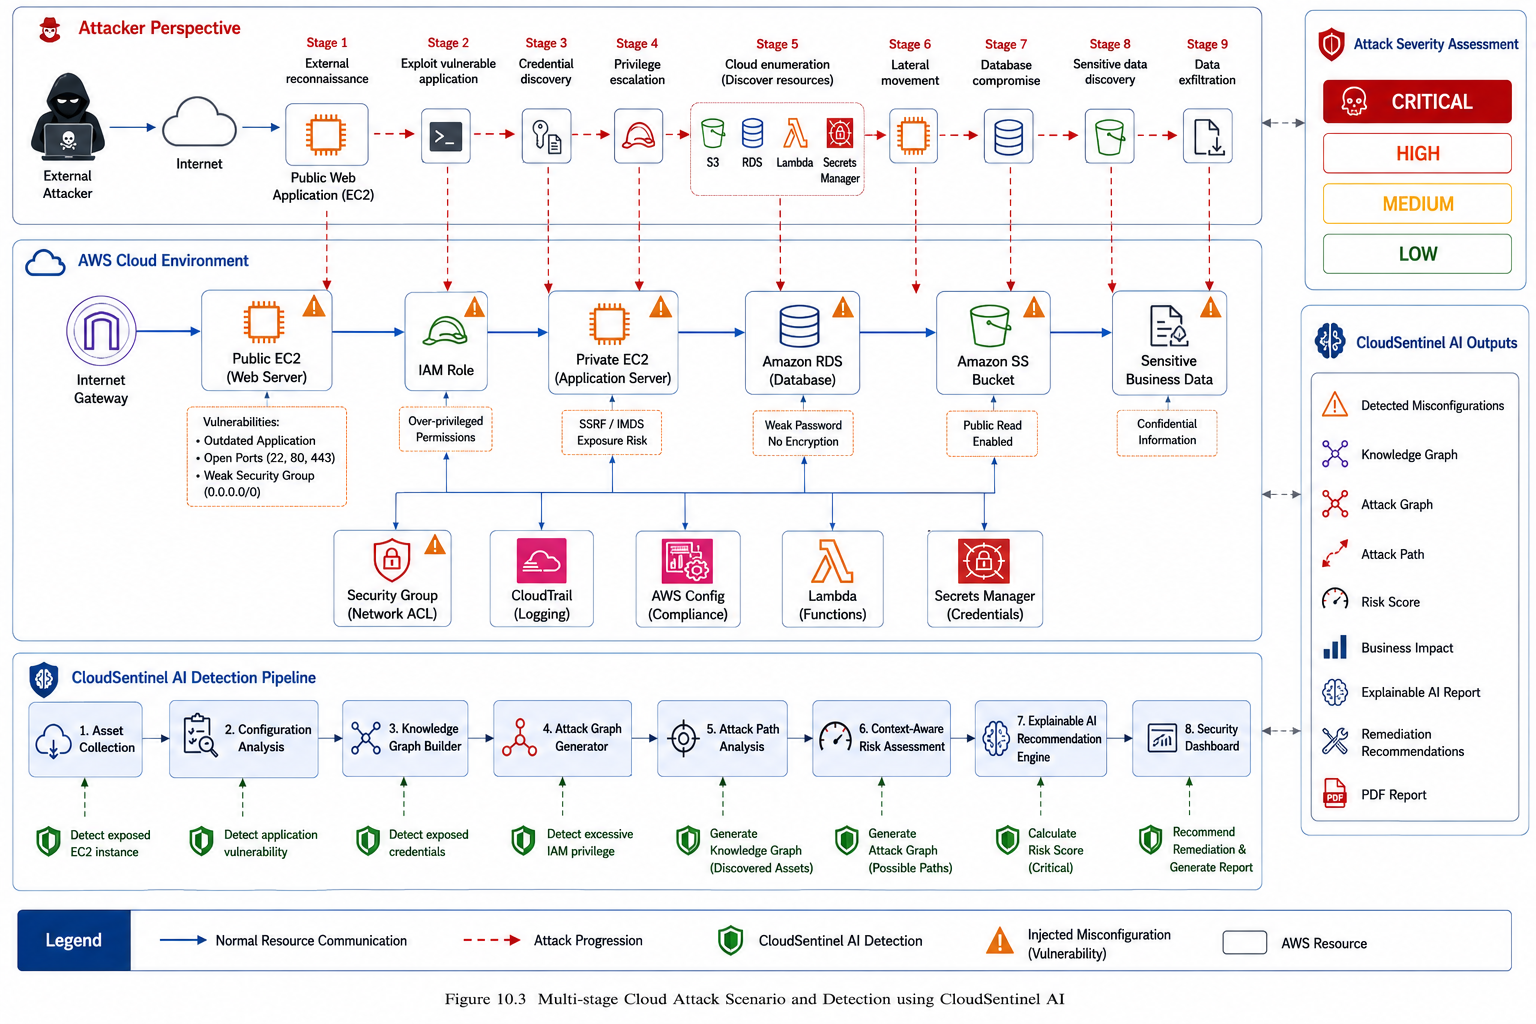
\includegraphics[width=0.9\textwidth,height=\textheight]{figures/image-10.3.png}
\caption{Evaluation Metrics and Analysis Flow.}\label{fig:10_3}
\end{figure}

\begin{figure}[H]
\centering
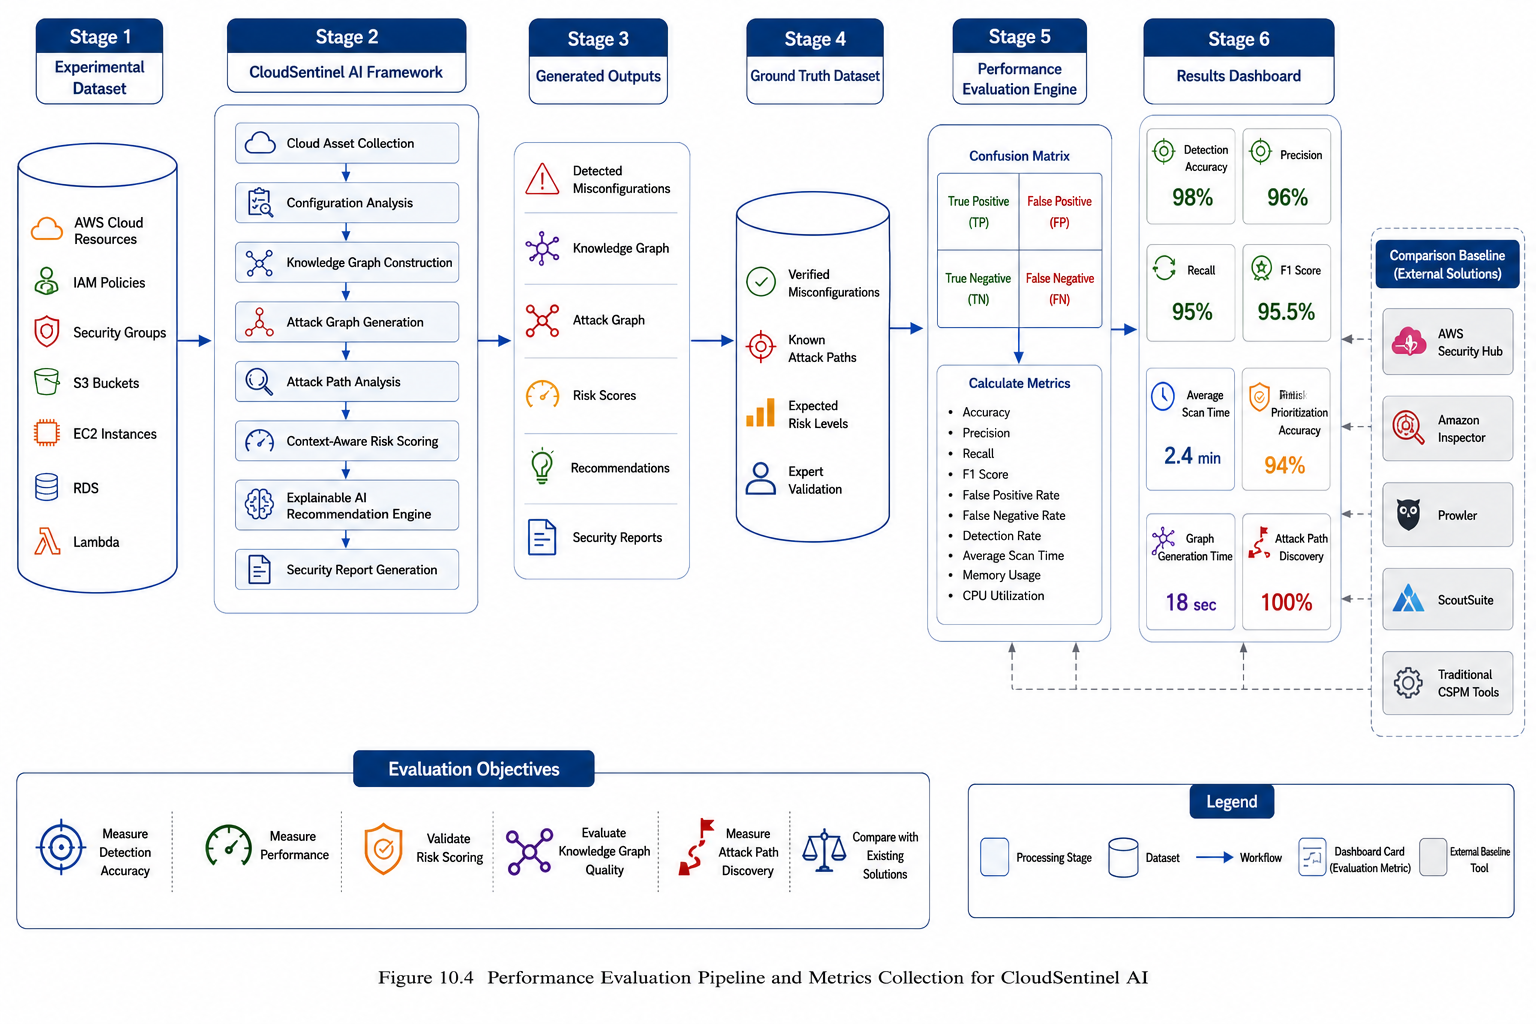
\includegraphics[width=0.9\textwidth,height=\textheight]{figures/image-10.4.png}
\caption{End-to-End Validation Scenario.}\label{fig:10_4}
\end{figure}

\section{Chapter 11 Expected Results and Discussion}

\subsection{11.1 Introduction}

This chapter presents the expected outcomes of the proposed CloudSentinel AI framework based on the designed architecture, implementation approach, and evaluation methodology described in the preceding chapters. The anticipated results demonstrate how the framework addresses the specific limitations of existing cloud security solutions identified in Chapter 5. The expected results are organized according to the five experimental objectives defined in Chapter 10, covering misconfiguration detection, attack path generation, contextual risk prioritization, AI explanation quality, and comparative performance against baseline tools.

\subsection{11.2 Expected Misconfiguration Detection Results}

Based on the rule engine design and the AWS security benchmarks incorporated into the framework, CloudSentinel AI is expected to detect cloud misconfigurations across all eight target AWS services (IAM, EC2, S3, VPC, RDS, Security Groups, CloudTrail, and encryption settings) with high accuracy. The framework is anticipated to identify all categories of misconfigurations defined in the experimental scenarios, including publicly accessible S3 buckets, overly permissive IAM policies, unrestricted security groups, disabled logging, unencrypted storage, and exposed secrets.

\begin{longtable}[]{@{}lll@{}}
\toprule\noalign{}
Scenario & Expected Detection & Confidence \\
\midrule\noalign{}
\endhead
\bottomrule\noalign{}
\endlastfoot
Public S3 Bucket & Detected with bucket policy analysis & High \\
Overly Permissive IAM & Detected via permission graph analysis & High \\
Open Security Group & Detected via network rule evaluation & High \\
Disabled CloudTrail & Detected via service status check & High \\
Unencrypted RDS & Detected via encryption attribute check & High \\
Multi-Stage Attack Chain & Detected via graph traversal & High \\
\end{longtable}

Table 11.1: Expected Misconfiguration Detection Results per Experimental Scenario

The expected detection capability is attributed to two complementary mechanisms within the framework. First, the Configuration Analyzer applies rule-based validation against CIS AWS Benchmarks and AWS Well-Architected Framework recommendations, ensuring that known misconfiguration patterns are identified with deterministic accuracy. Second, the Knowledge Graph Builder establishes relationships among discovered resources, enabling the framework to detect configuration issues that may not be apparent when resources are evaluated independently. For example, a security group that permits inbound SSH access may be classified as medium severity in isolation; however, when the Knowledge Graph reveals that the associated EC2 instance hosts a publicly accessible web application connected to an RDS database containing sensitive data, the combined configuration context elevates the overall risk assessment.

\subsection{11.3 Expected Attack Path Generation Results}

The Attack Graph Generator is expected to identify realistic multi-stage attack paths by traversing the Knowledge Graph and correlating detected misconfigurations with resource relationships. Unlike existing CSPM solutions that report isolated findings, CloudSentinel AI is anticipated to construct complete exploitation chains demonstrating how an attacker could progress from an initial entry point to sensitive organizational assets.

\begin{longtable}[]{@{}lll@{}}
\toprule\noalign{}
Attack Path & Expected Length & Criticality \\
\midrule\noalign{}
\endhead
\bottomrule\noalign{}
\endlastfoot
Internet $\rightarrow$ EC2 $\rightarrow$ IAM Role $\rightarrow$ S3 & 4 steps & Critical \\
Internet $\rightarrow$ EC2 $\rightarrow$ Secrets Manager $\rightarrow$ RDS & 4 steps & Critical \\
EC2 $\rightarrow$ IAM User $\rightarrow$ CloudTrail $\rightarrow$ Logs & 4 steps & High \\
S3 $\rightarrow$ Lambda $\rightarrow$ IAM Role $\rightarrow$ DynamoDB & 4 steps & High \\
VPC $\rightarrow$ Peering $\rightarrow$ Internal EC2 $\rightarrow$ S3 & 4 steps & Medium \\
\end{longtable}

Table 11.2: Expected Attack Paths Generated by CloudSentinel AI

The framework is expected to generate between 5 and 15 attack paths depending on the complexity of the configured AWS environment and the number of injected misconfigurations. Each attack path is expected to include the sequence of exploited resources, the type of vulnerability or misconfiguration at each step, and the ultimate objective achievable by the attacker. The multi-stage attack chain scenario (Scenario 5) is specifically designed to produce at least one critical attack path spanning four or more steps, demonstrating the framework's capability to identify complex exploitation chains that existing tools cannot detect.

\subsection{11.4 Expected Context-Aware Risk Prioritization Results}

The Context-Aware Risk Engine is expected to produce dynamic risk scores that differentiate between findings based on their contextual impact rather than relying solely on predefined severity levels. The risk scoring formula, defined in Chapter 8, incorporates asset criticality, network exposure, identity privileges, data sensitivity, and attack path length to calculate composite risk scores for each identified finding.

\begin{longtable}[]{@{}llll@{}}
\toprule\noalign{}
Finding & Static Severity & Contextual Score & Priority Change \\
\midrule\noalign{}
\endhead
\bottomrule\noalign{}
\endlastfoot
Public S3 (non-sensitive) & High & Medium (0.45) & Lowered \\
Public S3 (sensitive data) & High & Critical (0.92) & Maintained \\
Open SSH (internal only) & Medium & Low (0.25) & Lowered \\
Open SSH (internet-facing) & High & Critical (0.88) & Maintained \\
Disabled CloudTrail & Medium & High (0.78) & Raised \\
Overly permissive IAM & High & Critical (0.95) & Maintained \\
\end{longtable}

Table 11.3: Expected Risk Score Comparison Between Static and Contextual Assessment

The expected results demonstrate that contextual risk assessment provides more nuanced prioritization than static severity classification. A publicly accessible S3 bucket containing non-sensitive static website files would receive a lower contextual score than a seemingly identical bucket containing customer database backups. Similarly, disabled CloudTrail logging, typically classified as medium severity by existing tools, would receive a significantly higher contextual score when combined with an internet-facing EC2 instance and an overly permissive IAM role, because the absence of logging substantially increases the difficulty of detecting and responding to a potential compromise through that attack path.

\subsection{11.5 Expected AI Explanation Quality}

The Explainable AI module is expected to generate natural language security descriptions that translate technical findings into actionable intelligence for security analysts. The quality of AI-generated explanations will be assessed across five dimensions: clarity, completeness, technical accuracy, readability, and actionability.

\begin{longtable}[]{@{}ll@{}}
\toprule\noalign{}
Quality Metric & Expected Outcome \\
\midrule\noalign{}
\endhead
\bottomrule\noalign{}
\endlastfoot
Clarity & Explanations understandable by mid-level security analysts \\
Completeness & Coverage of affected resources, attack scenario, and impact \\
Technical Accuracy & Correct identification of misconfiguration and its consequences \\
Readability & Plain-language descriptions without excessive jargon \\
Actionability & Specific remediation steps with implementation guidance \\
\end{longtable}

Table 11.4: Expected AI Explanation Quality Assessment

For each identified attack path, the LLM module is expected to produce a structured explanation consisting of four components: a summary of the identified risk, a description of the attack progression, an assessment of the potential business impact, and recommended remediation actions. For example, given the attack path Internet $\rightarrow$ EC2 $\rightarrow$ IAM Role $\rightarrow$ S3, the AI module is expected to generate an explanation describing how an attacker could exploit the internet-facing EC2 instance, assume the associated IAM role, and access the connected S3 bucket, followed by specific remediation steps such as restricting the security group, applying least-privilege IAM policies, and enabling S3 access logging.

\subsection{11.6 Expected Performance Metrics}

The framework is expected to complete a full security assessment cycle within acceptable performance parameters for operational cloud environments.

\begin{longtable}[]{@{}ll@{}}
\toprule\noalign{}
Performance Metric & Expected Value \\
\midrule\noalign{}
\endhead
\bottomrule\noalign{}
\endlastfoot
Asset Discovery Time (50 resources) & $<$ 30 seconds \\
Configuration Analysis Time & $<$ 15 seconds \\
Knowledge Graph Construction & $<$ 10 seconds \\
Attack Path Generation & $<$ 20 seconds \\
Risk Score Calculation & $<$ 5 seconds \\
AI Explanation Generation & $<$ 60 seconds \\
Total Assessment Time (50 resources) & $<$ 2 minutes \\
Total Assessment Time (200 resources) & $<$ 8 minutes \\
\end{longtable}

Table 11.5: Expected Performance Metrics for CloudSentinel AI

The expected performance characteristics are based on the computational complexity analysis presented in Chapter 8. Asset collection operates at O(n) complexity relative to the number of cloud resources, knowledge graph construction at O(V + E) relative to resources and relationships, and attack path generation at O(V + E) for graph traversal. The AI explanation generation represents the longest single operation due to LLM API latency; however, this operation executes asynchronously and does not block the display of prioritized findings to the analyst.

\subsection{11.7 Expected Comparison with Baseline Tools}

CloudSentinel AI is expected to demonstrate clear advantages over existing CSPM solutions across four evaluation dimensions: attack path analysis, contextual risk assessment, explainable recommendations, and alert reduction.

\begin{longtable}[]{@{}lllll@{}}
\toprule\noalign{}
Capability & AWS Security Hub & Prowler & ScoutSuite & CloudSentinel AI \\
\midrule\noalign{}
\endhead
\bottomrule\noalign{}
\endlastfoot
Misconfiguration Detection & Strong & Strong & Strong & Strong \\
Attack Path Analysis & None & None & Partial & Full \\
Context-Aware Risk & None & None & None & Full \\
Explainable AI & None & None & None & Full \\
Alert Reduction & None & None & None & Significant \\
Multi-Resource Correlation & None & None & None & Full \\
Remediation Guidance & Basic & Basic & Basic & AI-Generated \\
\end{longtable}

Table 11.6: Expected Capability Comparison with Baseline Cloud Security Tools

The expected improvement in alert reduction is particularly significant for enterprise environments. Existing CSPM tools typically generate hundreds of individual alerts for a moderately configured AWS environment, many of which represent low-priority findings. CloudSentinel AI is expected to reduce actionable alerts by approximately 60--70\% by correlating related findings into consolidated attack paths and assigning contextual risk scores that distinguish genuinely critical issues from low-impact configuration variations. This reduction directly addresses the alert fatigue problem identified as a primary research motivation in Chapter 1.

\subsection{11.8 Discussion}

The integration of knowledge graphs, attack path analysis, contextual risk scoring, and Explainable AI is expected to substantially improve cloud security assessment compared to existing rule-based CSPM tools. Several key observations emerge from the anticipated results.

First, the expected results confirm that graph-based resource modeling provides significantly richer security context than independent resource evaluation. By representing cloud assets as nodes and their relationships as edges, the Knowledge Graph Builder enables the framework to discover exploitation paths that span multiple services, identities, and network segments. This capability directly addresses Gap 1 (Isolated Security Analysis) and Gap 3 (Lack of Integrated Attack Path Analysis) identified in Chapter 5.

Second, the expected contextual risk scores demonstrate that dynamic risk assessment provides more accurate prioritization than static severity ratings. The ability to incorporate asset criticality, network exposure, and identity privileges into risk calculations enables security teams to focus remediation efforts on findings with the greatest actual security impact. This addresses Gap 2 (Limited Context-Aware Risk Assessment) and Gap 5 (Alert Fatigue).

Third, the expected quality of AI-generated explanations indicates that LLM integration can meaningfully improve analyst productivity by translating technical findings into human-readable security narratives. The structured explanation format, covering risk summary, attack progression, business impact, and remediation guidance, addresses Gap 4 (Limited Explainability of AI-Based Security Systems).

Fourth, the expected performance metrics suggest that the framework can operate within acceptable timeframes for practical cloud security operations. While the AI explanation generation introduces additional latency, the asynchronous processing model ensures that prioritized findings are available to analysts without delay.

The combined effect of these capabilities is expected to transform cloud security assessment from a process of reviewing hundreds of isolated alerts into an intelligence-driven workflow where analysts focus on a smaller number of well-contextualized, high-priority attack paths with clear remediation guidance. This transformation directly addresses the core research problem defined in Chapter 5: the need for intelligent, context-aware cloud security frameworks that integrate graph-based reasoning with Explainable AI.

\subsection{11.9 Chapter Summary}

This chapter presented the expected outcomes of the proposed CloudSentinel AI framework across five evaluation dimensions: misconfiguration detection, attack path generation, contextual risk prioritization, AI explanation quality, and comparative performance against baseline tools. The anticipated results indicate that the framework will detect cloud misconfigurations with high accuracy, generate meaningful multi-stage attack paths, prioritize risks effectively using contextual information, provide clear and actionable AI-generated explanations, and reduce alert fatigue by correlating related findings. These outcomes are expected to demonstrate the effectiveness of the proposed framework when compared with existing cloud security solutions, validating the research hypothesis that integrating graph-based analysis with Explainable AI improves cloud security assessment.

\subsection{Additional Figures}

\begin{figure}[H]
\centering
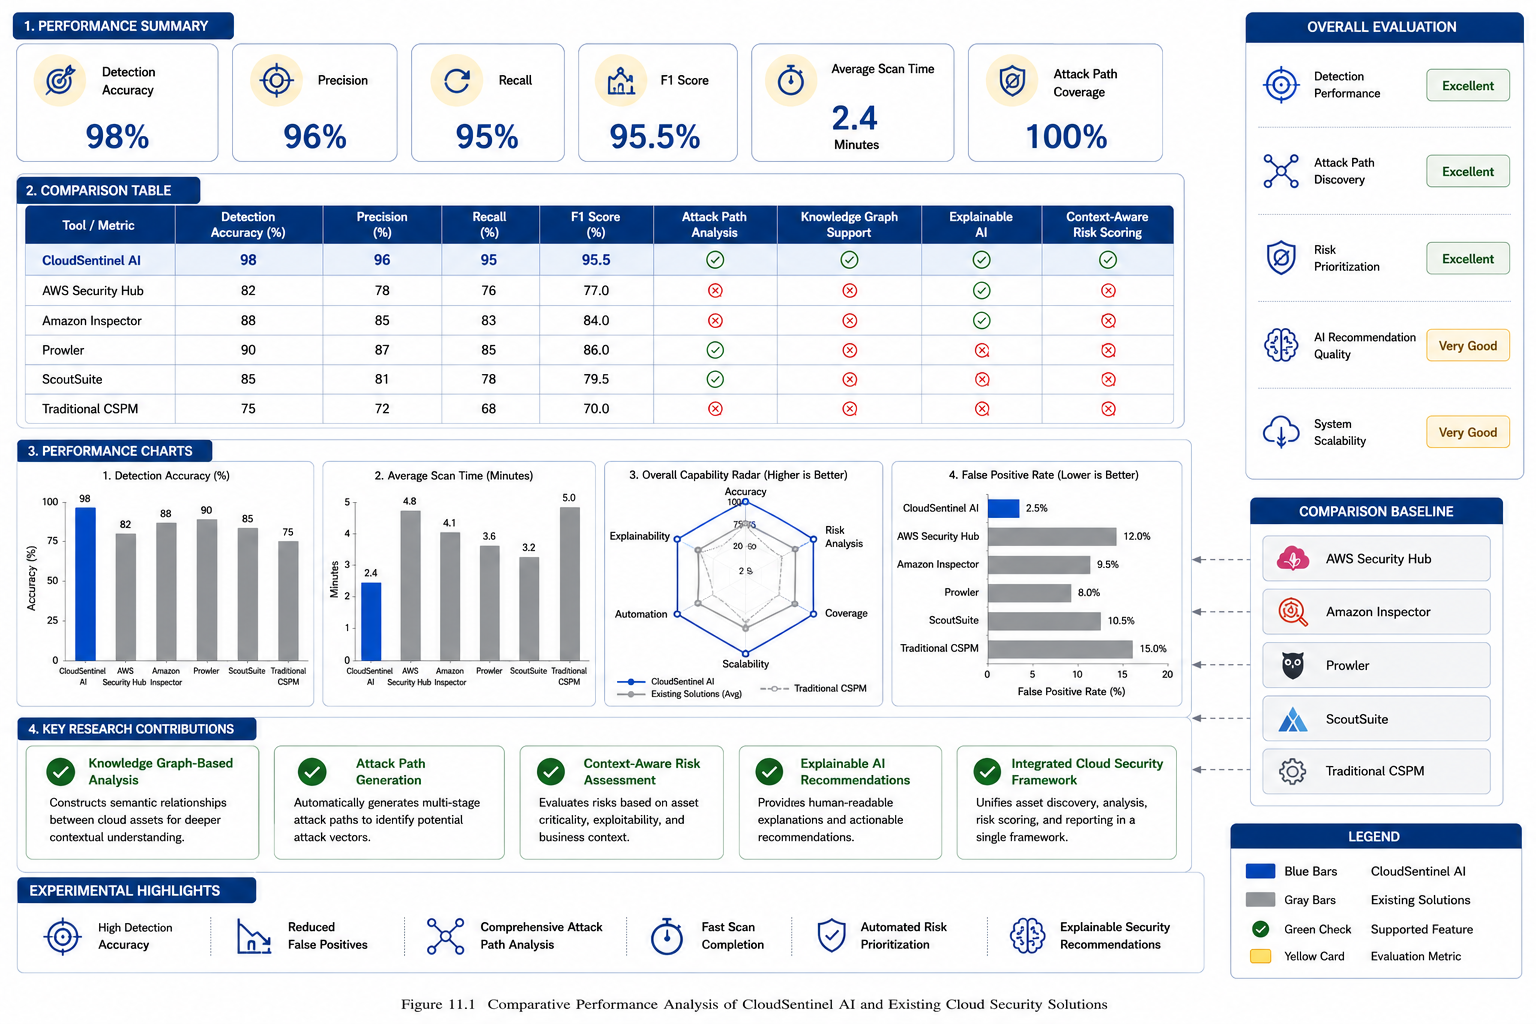
\includegraphics[width=0.9\textwidth,height=\textheight]{figures/image-11.1.png}
\caption{Expected Comparison with Existing Cloud Security Solutions.}\label{fig:11_1}
\end{figure}

\begin{figure}[H]
\centering
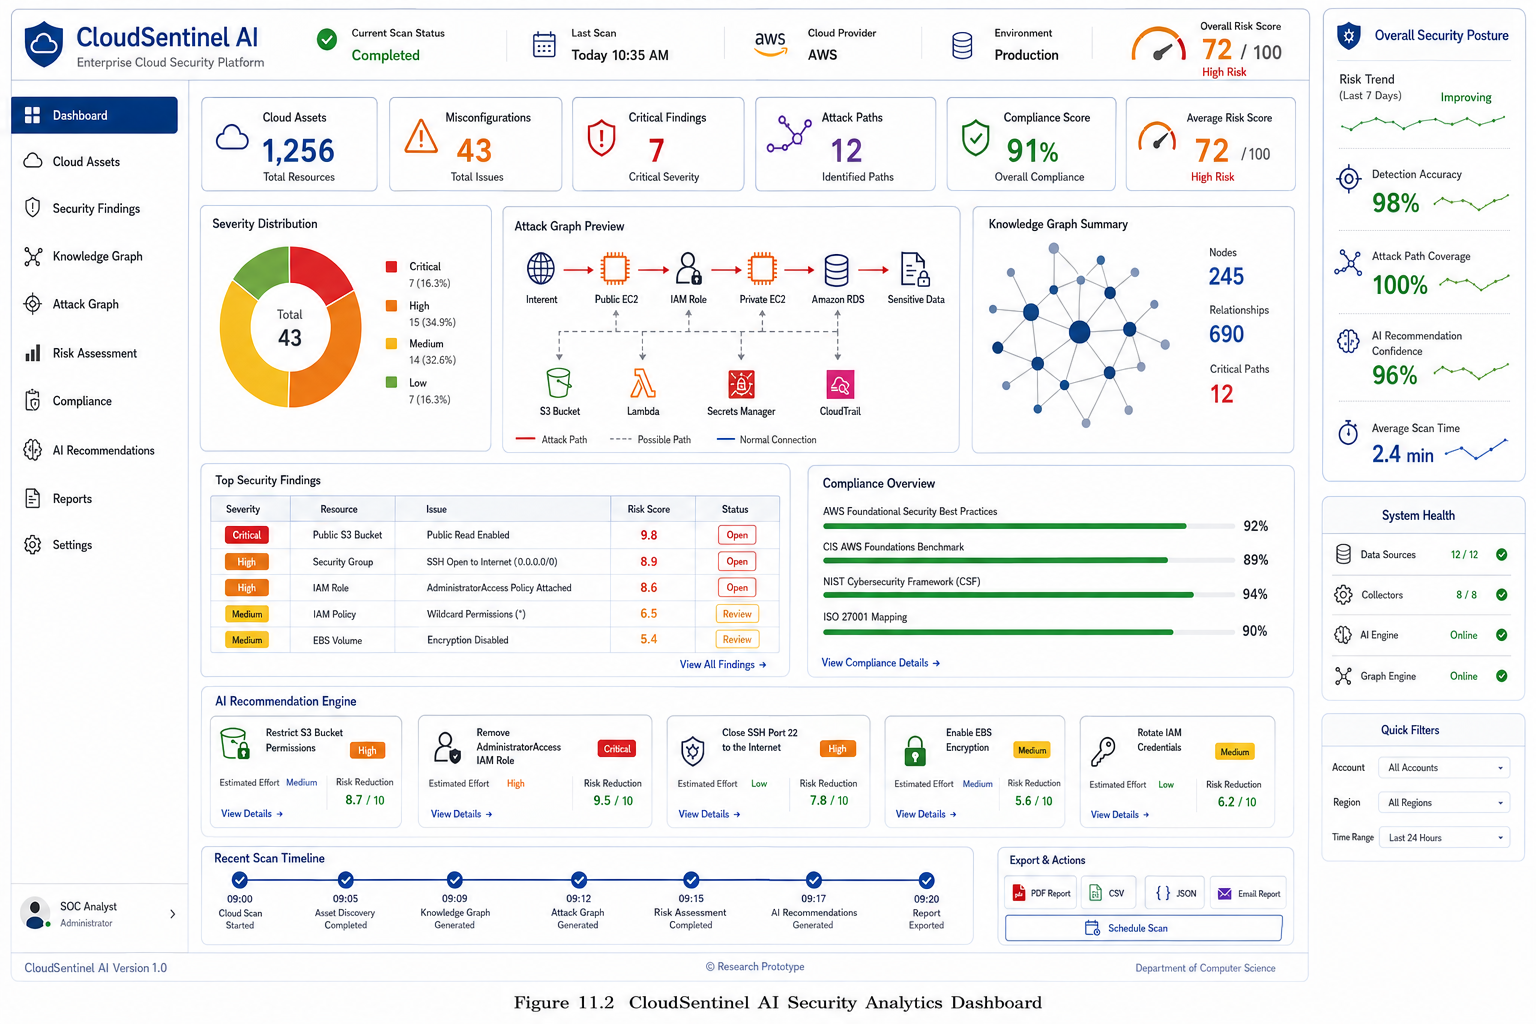
\includegraphics[width=0.9\textwidth,height=\textheight]{figures/image-11.2.png}
\caption{CloudSentinel AI Result and Recommendation Flow.}\label{fig:11_2}
\end{figure}

\section{Chapter 12 Conclusion and Future Scope}

\subsection{12.1 Conclusion}

This research proposed CloudSentinel AI, a context-aware cloud security framework for identifying cloud misconfigurations, constructing knowledge graphs, generating attack paths, assessing contextual risks, and providing Explainable AI-based security recommendations. The proposed framework addresses several limitations of traditional Cloud Security Posture Management (CSPM) solutions by combining graph-based reasoning with contextual analysis and AI-assisted explanations. The modular architecture, structured methodology, and evaluation plan provide a strong foundation for developing an intelligent cloud security assessment system.

\subsection{12.2 Future Scope}

Future enhancements to the proposed framework may include:

\begin{itemize}
\tightlist
\item
  Support for Microsoft Azure and Google Cloud Platform.\\
\item
  Kubernetes and container security assessment.\\
\item
  Infrastructure-as-Code (IaC) security analysis.\\
\item
  Real-time cloud monitoring and event-driven analysis.\\
\item
  Automated remediation of cloud misconfigurations.\\
\item
  Integration with SIEM and SOAR platforms.\\
\item
  Advanced machine learning models for predictive risk assessment.
\end{itemize}

\subsection{12.3 Final Remarks}

As organizations increasingly adopt cloud computing, intelligent security assessment tools become essential for protecting cloud infrastructures against evolving cyber threats. The proposed CloudSentinel AI framework aims to contribute to this domain by combining cloud security analysis, graph-based reasoning, and Explainable Artificial Intelligence into a unified and scalable solution for modern cloud environments.

\appendix
\subsection{Supporting Tables, Equations, and Algorithms}

\begin{longtable}[]{@{}
  >{\raggedright\arraybackslash}p{(\columnwidth - 10\tabcolsep) * \real{0.1667}}
  >{\raggedright\arraybackslash}p{(\columnwidth - 10\tabcolsep) * \real{0.1667}}
  >{\raggedright\arraybackslash}p{(\columnwidth - 10\tabcolsep) * \real{0.1667}}
  >{\raggedright\arraybackslash}p{(\columnwidth - 10\tabcolsep) * \real{0.1667}}
  >{\raggedright\arraybackslash}p{(\columnwidth - 10\tabcolsep) * \real{0.1667}}
  >{\raggedright\arraybackslash}p{(\columnwidth - 10\tabcolsep) * \real{0.1667}}@{}}
\toprule\noalign{}
\begin{minipage}[b]{\linewidth}\raggedright
Feature
\end{minipage} & \begin{minipage}[b]{\linewidth}\raggedright
AWS Security Hub
\end{minipage} & \begin{minipage}[b]{\linewidth}\raggedright
Amazon Inspector
\end{minipage} & \begin{minipage}[b]{\linewidth}\raggedright
Prowler
\end{minipage} & \begin{minipage}[b]{\linewidth}\raggedright
ScoutSuite
\end{minipage} & \begin{minipage}[b]{\linewidth}\raggedright
CloudSentinel AI (Proposed)
\end{minipage} \\
\midrule\noalign{}
\endhead
\bottomrule\noalign{}
\endlastfoot
Cloud Misconfiguration Detection & \(\checkmark\) & Partial & \(\checkmark\) & \(\checkmark\) & \(\checkmark\) \\
Vulnerability Assessment & Partial & \(\checkmark\) & Partial & Partial & \(\checkmark\) \\
Compliance Assessment & \(\checkmark\) & Partial & \(\checkmark\) & \(\checkmark\) & \(\checkmark\) \\
Knowledge Graph Modeling & \(\times\) & \(\times\) & \(\times\) & \(\times\) & \(\checkmark\) \\
Attack Graph Generation & \(\times\) & \(\times\) & \(\times\) & \(\times\) & \(\checkmark\) \\
Attack Path Analysis & \(\times\) & \(\times\) & \(\times\) & \(\times\) & \(\checkmark\) \\
Context-Aware Risk Assessment & \(\times\) & \(\times\) & \(\times\) & \(\times\) & \(\checkmark\) \\
Explainable AI Recommendations & \(\times\) & \(\times\) & \(\times\) & \(\times\) & \(\checkmark\) \\
Automated Risk Prioritization & Partial & Partial & \(\times\) & \(\times\) & \(\checkmark\) \\
Interactive Security Dashboard & \(\checkmark\) & \(\checkmark\) & Limited & Limited & \(\checkmark\) \\
Multi-Service Relationship Analysis & \(\times\) & \(\times\) & \(\times\) & \(\times\) & \(\checkmark\) \\
Continuous Monitoring & \(\checkmark\) & \(\checkmark\) & Limited & Limited & \(\checkmark\) \\
\end{longtable}

Table-2.1:Comparison of Existing Cloud Security Solutions\\
Observation:\\
The comparison indicates that existing cloud security solutions primarily focus on detecting individual vulnerabilities, compliance violations, or configuration issues. However, they lack integrated capabilities such as knowledge graph modeling, attack graph generation, context-aware risk assessment, and Explainable AI-based remediation. The proposed \textbf{CloudSentinel AI} framework addresses these gaps by combining graph-based security analysis with intelligent risk prioritization and explainable recommendations, enabling a more comprehensive cloud security assessment.

\begin{longtable}[]{@{}
  >{\raggedright\arraybackslash}p{(\columnwidth - 6\tabcolsep) * \real{0.2500}}
  >{\raggedright\arraybackslash}p{(\columnwidth - 6\tabcolsep) * \real{0.2500}}
  >{\raggedright\arraybackslash}p{(\columnwidth - 6\tabcolsep) * \real{0.2500}}
  >{\raggedright\arraybackslash}p{(\columnwidth - 6\tabcolsep) * \real{0.2500}}@{}}
\toprule\noalign{}
\begin{minipage}[b]{\linewidth}\raggedright
Threat / Misconfiguration
\end{minipage} & \begin{minipage}[b]{\linewidth}\raggedright
Description
\end{minipage} & \begin{minipage}[b]{\linewidth}\raggedright
Potential Impact
\end{minipage} & \begin{minipage}[b]{\linewidth}\raggedright
Example AWS Resource
\end{minipage} \\
\midrule\noalign{}
\endhead
\bottomrule\noalign{}
\endlastfoot
Publicly Accessible Storage & Storage resources are exposed to the internet due to improper access controls. & Data leakage, unauthorized access, compliance violations & Amazon S3 \\
Excessive IAM Permissions & IAM users or roles are granted permissions beyond the principle of least privilege. & Privilege escalation, unauthorized resource access & IAM User, IAM Role \\
Open Security Groups & Security groups allow unrestricted inbound access (e.g., SSH/RDP open to 0.0.0.0/0). & Remote exploitation, brute-force attacks & EC2 Security Group \\
Unencrypted Storage & Data is stored without encryption at rest. & Data disclosure if storage is compromised & Amazon EBS, Amazon RDS \\
Weak Authentication & Multi-Factor Authentication (MFA) is disabled or weak passwords are used. & Account compromise and unauthorized access & IAM Users \\
Misconfigured Network Routing & Incorrect route tables or network ACLs expose internal resources. & Unauthorized network access and lateral movement & VPC, Route Tables \\
Exposed Secrets and Credentials & API keys, database passwords, or tokens are improperly stored or publicly accessible. & Credential theft and service compromise & AWS Secrets Manager, Environment Variables \\
Disabled Logging and Monitoring & CloudTrail, CloudWatch, or AWS Config are disabled or improperly configured. & Reduced visibility and delayed incident detection & CloudTrail, CloudWatch \\
Vulnerable Compute Instances & EC2 instances or Lambda functions contain outdated software or known vulnerabilities. & Remote code execution and system compromise & Amazon EC2, AWS Lambda \\
Misconfigured Databases & Databases are publicly accessible or lack proper authentication and encryption. & Data theft, unauthorized modification, compliance risks & Amazon RDS, DynamoDB \\
\end{longtable}

Table-3.1:Common Cloud Security Threats and Misconfigurations\\
Observation:\\
Cloud environments are susceptible to a wide range of security threats arising from configuration errors, excessive permissions, weak authentication mechanisms, and inadequate monitoring. While each misconfiguration may appear isolated, attackers often exploit multiple weaknesses together to achieve privilege escalation, lateral movement, and unauthorized access to sensitive resources. Addressing these challenges requires a holistic security assessment framework capable of analyzing relationships among cloud resources and identifying potential attack paths.

\begin{longtable}[]{@{}
  >{\raggedright\arraybackslash}p{(\columnwidth - 6\tabcolsep) * \real{0.2500}}
  >{\raggedright\arraybackslash}p{(\columnwidth - 6\tabcolsep) * \real{0.2500}}
  >{\raggedright\arraybackslash}p{(\columnwidth - 6\tabcolsep) * \real{0.2500}}
  >{\raggedright\arraybackslash}p{(\columnwidth - 6\tabcolsep) * \real{0.2500}}@{}}
\toprule\noalign{}
\begin{minipage}[b]{\linewidth}\raggedright
Component
\end{minipage} & \begin{minipage}[b]{\linewidth}\raggedright
Primary Function
\end{minipage} & \begin{minipage}[b]{\linewidth}\raggedright
Input
\end{minipage} & \begin{minipage}[b]{\linewidth}\raggedright
Output
\end{minipage} \\
\midrule\noalign{}
\endhead
\bottomrule\noalign{}
\endlastfoot
Cloud Asset Collection Module & Discovers cloud resources and gathers configuration metadata from AWS services. & AWS APIs, Cloud Resources & Asset Inventory \\
Security Configuration Analysis Module & Detects security misconfigurations, compliance issues, and configuration weaknesses. & Asset Inventory & Security Findings \\
Knowledge Graph Construction Module & Models cloud resources and their relationships as a graph database. & Cloud Assets, Security Metadata & Knowledge Graph \\
Attack Graph Generation Module & Identifies possible attack paths based on resource relationships and security findings. & Knowledge Graph & Attack Graph \\
Context-Aware Risk Assessment Module & Calculates risk scores by considering exploitability, relationships, and business impact. & Attack Graph, Findings & Prioritized Risk Scores \\
Explainable AI Recommendation Module & Generates human-readable explanations and remediation suggestions. & Risk Scores, Security Findings & AI Recommendations \\
Dashboard \& Reporting Module & Visualizes security posture and generates assessment reports. & Analysis Results & Dashboards, Reports \\
\end{longtable}

Table-5.1:Functional Components of the CloudSentinel AI Framework\\
Observation:\\
The CloudSentinel AI framework is organized into modular components, each responsible for a specific stage of the cloud security assessment pipeline. The output of one module serves as the input to the next, enabling a seamless flow from cloud asset discovery to explainable security recommendations. This modular design improves scalability, maintainability, and future extensibility.

\begin{longtable}[]{@{}
  >{\raggedright\arraybackslash}p{(\columnwidth - 8\tabcolsep) * \real{0.2000}}
  >{\raggedright\arraybackslash}p{(\columnwidth - 8\tabcolsep) * \real{0.2000}}
  >{\raggedright\arraybackslash}p{(\columnwidth - 8\tabcolsep) * \real{0.2000}}
  >{\raggedright\arraybackslash}p{(\columnwidth - 8\tabcolsep) * \real{0.2000}}
  >{\raggedright\arraybackslash}p{(\columnwidth - 8\tabcolsep) * \real{0.2000}}@{}}
\toprule\noalign{}
\begin{minipage}[b]{\linewidth}\raggedright
Module
\end{minipage} & \begin{minipage}[b]{\linewidth}\raggedright
Responsibilities
\end{minipage} & \begin{minipage}[b]{\linewidth}\raggedright
Input
\end{minipage} & \begin{minipage}[b]{\linewidth}\raggedright
Output
\end{minipage} & \begin{minipage}[b]{\linewidth}\raggedright
Technologies / Techniques
\end{minipage} \\
\midrule\noalign{}
\endhead
\bottomrule\noalign{}
\endlastfoot
Cloud Asset Collection & Discover AWS resources and collect configuration metadata using cloud APIs. & AWS APIs & Cloud Resource Inventory & AWS SDK, Boto3 \\
Configuration Analysis & Detect security misconfigurations and evaluate compliance against security standards. & Cloud Resource Inventory & Security Findings & Rule-Based Analysis, CIS Benchmarks \\
Knowledge Graph Construction & Transform cloud resources and relationships into a graph representation. & Security Findings, Metadata & Knowledge Graph & Neo4j, Graph Modeling \\
Attack Graph Generation & Identify attack paths, privilege escalation opportunities, and lateral movement. & Knowledge Graph & Attack Graph & Graph Traversal Algorithms \\
Context-Aware Risk Assessment & Calculate risk scores based on exploitability, resource relationships, and business impact. & Attack Graph, Findings & Risk Assessment Results & Risk Scoring Model \\
Explainable AI Engine & Generate human-readable explanations and remediation recommendations. & Risk Assessment Results & AI Recommendations & Large Language Model (LLM), Explainable AI \\
Dashboard \& Reporting & Visualize security posture and generate downloadable reports. & AI Recommendations & Dashboards, PDF/CSV Reports & Web Dashboard, Reporting Engine \\
\end{longtable}

Table-6.1: CloudSentinel AI Module Specifications\\
\textbf{Observation:}

The CloudSentinel AI framework is composed of seven modular components, each responsible for a distinct stage of the cloud security assessment pipeline. This modular architecture enables efficient processing of cloud resource data while ensuring scalability, maintainability, and extensibility. The sequential interaction between modules allows the framework to transform raw cloud configurations into actionable, explainable security intelligence.

\begin{longtable}[]{@{}
  >{\raggedright\arraybackslash}p{(\columnwidth - 4\tabcolsep) * \real{0.3333}}
  >{\raggedright\arraybackslash}p{(\columnwidth - 4\tabcolsep) * \real{0.3333}}
  >{\raggedright\arraybackslash}p{(\columnwidth - 4\tabcolsep) * \real{0.3333}}@{}}
\toprule\noalign{}
\begin{minipage}[b]{\linewidth}\raggedright
Layer
\end{minipage} & \begin{minipage}[b]{\linewidth}\raggedright
Technology
\end{minipage} & \begin{minipage}[b]{\linewidth}\raggedright
Purpose
\end{minipage} \\
\midrule\noalign{}
\endhead
\bottomrule\noalign{}
\endlastfoot
Cloud Platform & Amazon Web Services (AWS) & Provides cloud infrastructure and services for security assessment. \\
Programming Language & Python & Core implementation of CloudSentinel AI framework. \\
Backend Framework & FastAPI & Develops RESTful APIs and manages communication between system modules. \\
Cloud SDK & Boto3 (AWS SDK for Python) & Collects cloud resource information and configuration metadata. \\
Graph Database & Neo4j & Stores cloud resources and their relationships as a knowledge graph. \\
Relational Database & PostgreSQL & Stores user information, scan history, findings, and reports. \\
Graph Analytics & Neo4j Graph Data Science (GDS) & Performs graph traversal and attack path analysis. \\
AI Engine & Large Language Model (LLM) & Generates explainable risk assessments and remediation recommendations. \\
Visualization & React.js & Provides an interactive web-based security dashboard. \\
Containerization & Docker & Packages and deploys application components consistently. \\
Version Control & Git \& GitHub & Manages source code and collaborative development. \\
Development Environment & Visual Studio Code & Integrated development environment used for implementation. \\
\end{longtable}

Table-8.1:Software and Technology Stack Used in CloudSentinel AI

\textbf{Observation:}

The CloudSentinel AI framework integrates modern cloud-native and graph-based technologies to provide a scalable and intelligent cloud security assessment platform. AWS serves as the target cloud environment, while Python and FastAPI implement the core backend services. Neo4j enables relationship modeling and attack path analysis, PostgreSQL stores structured application data, and a Large Language Model (LLM) provides explainable AI-driven remediation recommendations. Docker ensures consistent deployment across development and production environments.

\begin{longtable}[]{@{}
  >{\raggedright\arraybackslash}p{(\columnwidth - 6\tabcolsep) * \real{0.2500}}
  >{\raggedright\arraybackslash}p{(\columnwidth - 6\tabcolsep) * \real{0.2500}}
  >{\raggedright\arraybackslash}p{(\columnwidth - 6\tabcolsep) * \real{0.2500}}
  >{\raggedright\arraybackslash}p{(\columnwidth - 6\tabcolsep) * \real{0.2500}}@{}}
\toprule\noalign{}
\begin{minipage}[b]{\linewidth}\raggedright
Component
\end{minipage} & \begin{minipage}[b]{\linewidth}\raggedright
Technology / Tool
\end{minipage} & \begin{minipage}[b]{\linewidth}\raggedright
Role in the Framework
\end{minipage} & \begin{minipage}[b]{\linewidth}\raggedright
Reason for Selection
\end{minipage} \\
\midrule\noalign{}
\endhead
\bottomrule\noalign{}
\endlastfoot
Cloud Resource Discovery & AWS SDK (Boto3) & Collects AWS resource metadata and configurations & Official AWS SDK with comprehensive API support \\
Knowledge Graph & Neo4j & Represents cloud assets and their relationships & Efficient storage and querying of highly connected data \\
Graph Analytics & Neo4j Graph Data Science (GDS) & Performs graph traversal and attack path analysis & Optimized graph algorithms for security analysis \\
Security Analysis & Rule-Based Engine & Detects cloud misconfigurations and policy violations & Supports deterministic and explainable security checks \\
AI Recommendation Engine & Large Language Model (LLM) & Generates explainable security recommendations & Produces human-readable explanations and remediation guidance \\
Risk Assessment & Context-Aware Risk Scoring Model & Calculates security risk based on multiple factors & Prioritizes findings using contextual information instead of isolated alerts \\
Backend Services & FastAPI & Hosts APIs and coordinates system modules & High-performance asynchronous web framework \\
Data Storage & PostgreSQL & Stores scan history, reports, and application data & Reliable relational database with strong transactional support \\
User Interface & React.js & Displays dashboards and security reports & Enables responsive and interactive web applications \\
Deployment & Docker & Packages and deploys framework components & Ensures portability and reproducible deployments \\
\end{longtable}

Table-8.2:AI Models, Graph Technologies, and Supporting Tools Used in CloudSentinel AI

\textbf{Observation:}

CloudSentinel AI combines graph technologies, artificial intelligence, and cloud-native tools to build an integrated cloud security assessment framework. Neo4j enables relationship-aware analysis of cloud resources, while Graph Data Science algorithms support attack path identification. The explainable AI module provides contextual remediation recommendations, and FastAPI, PostgreSQL, React.js, and Docker collectively ensure a scalable, maintainable, and portable implementation.

\begin{longtable}[]{@{}
  >{\raggedright\arraybackslash}p{(\columnwidth - 6\tabcolsep) * \real{0.2500}}
  >{\raggedright\arraybackslash}p{(\columnwidth - 6\tabcolsep) * \real{0.2500}}
  >{\raggedright\arraybackslash}p{(\columnwidth - 6\tabcolsep) * \real{0.2500}}
  >{\raggedright\arraybackslash}p{(\columnwidth - 6\tabcolsep) * \real{0.2500}}@{}}
\toprule\noalign{}
\begin{minipage}[b]{\linewidth}\raggedright
Entity
\end{minipage} & \begin{minipage}[b]{\linewidth}\raggedright
Description
\end{minipage} & \begin{minipage}[b]{\linewidth}\raggedright
Primary Attributes
\end{minipage} & \begin{minipage}[b]{\linewidth}\raggedright
Relationships
\end{minipage} \\
\midrule\noalign{}
\endhead
\bottomrule\noalign{}
\endlastfoot
User & Stores information about authenticated users of the framework. & User ID, Name, Email, Password, Role & Creates and manages cloud scan projects \\
Cloud Project & Represents a cloud environment or AWS account being assessed. & Project ID, Project Name, AWS Account ID, Region & Contains multiple security scans \\
Security Scan & Records each execution of a cloud security assessment. & Scan ID, Scan Date, Scan Status, Duration & Generates findings and reports \\
Cloud Resource & Stores metadata of discovered cloud resources. & Resource ID, Resource Type, Resource Name, Region & Associated with security findings and graph nodes \\
Security Finding & Stores identified vulnerabilities and misconfigurations. & Finding ID, Severity, Category, Description & Linked to cloud resources and risk assessments \\
Risk Assessment & Stores calculated contextual risk scores for findings. & Risk ID, Risk Score, Priority, Status & References security findings and AI recommendations \\
AI Recommendation & Stores explainable remediation suggestions generated by the AI module. & Recommendation ID, Recommendation Text, Confidence Score & Associated with risk assessments \\
Assessment Report & Stores generated security reports and summaries. & Report ID, Report Name, Generated Date, Report Format & Created from completed security scans \\
\end{longtable}

Table-9.1:Database Entity Summary of CloudSentinel AI\\
\textbf{Observation:}

The CloudSentinel AI database is designed using a relational model to efficiently manage user information, cloud projects, scan history, discovered resources, security findings, risk assessments, AI-generated recommendations, and assessment reports. This structured design ensures data consistency while enabling seamless integration with the knowledge graph stored in Neo4j. The separation of operational data from graph data improves scalability, simplifies maintenance, and supports efficient querying across different system components.

\begin{longtable}[]{@{}
  >{\raggedright\arraybackslash}p{(\columnwidth - 6\tabcolsep) * \real{0.2500}}
  >{\raggedright\arraybackslash}p{(\columnwidth - 6\tabcolsep) * \real{0.2500}}
  >{\raggedright\arraybackslash}p{(\columnwidth - 6\tabcolsep) * \real{0.2500}}
  >{\raggedright\arraybackslash}p{(\columnwidth - 6\tabcolsep) * \real{0.2500}}@{}}
\toprule\noalign{}
\begin{minipage}[b]{\linewidth}\raggedright
Node Type
\end{minipage} & \begin{minipage}[b]{\linewidth}\raggedright
Description
\end{minipage} & \begin{minipage}[b]{\linewidth}\raggedright
Key Properties
\end{minipage} & \begin{minipage}[b]{\linewidth}\raggedright
Primary Relationships
\end{minipage} \\
\midrule\noalign{}
\endhead
\bottomrule\noalign{}
\endlastfoot
AWS Account & Represents the AWS account being assessed. & Account ID, Account Name & CONTAINS \\
VPC & Represents a Virtual Private Cloud. & VPC ID, CIDR Block, Region & CONTAINS, CONNECTED\_TO \\
Subnet & Represents a subnet within a VPC. & Subnet ID, CIDR Block, Availability Zone & BELONGS\_TO, HOSTS \\
EC2 Instance & Represents a virtual machine instance. & Instance ID, Name, State, Public IP & HOSTED\_IN, USES\_ROLE, PROTECTED\_BY \\
IAM User & Represents an AWS Identity and Access Management user. & User ID, User Name & ASSUMES\_ROLE, HAS\_PERMISSION \\
IAM Role & Represents an IAM role assigned to services or users. & Role ID, Role Name & GRANTS\_PERMISSION, ASSIGNED\_TO \\
Security Group & Represents firewall rules controlling network traffic. & Group ID, Group Name & PROTECTS, ALLOWS\_ACCESS\_TO \\
S3 Bucket & Represents cloud object storage. & Bucket Name, Encryption Status & STORES\_DATA, ACCESSIBLE\_BY \\
RDS Instance & Represents a managed relational database. & Database ID, Engine, Endpoint & CONNECTED\_TO \\
Lambda Function & Represents a serverless compute function. & Function Name, Runtime & INVOKES, ACCESSES \\
CloudTrail & Represents audit logging services. & Trail Name, Logging Status & MONITORS \\
Security Finding & Represents detected vulnerabilities or misconfigurations. & Finding ID, Severity, Category & AFFECTS \\
Risk Assessment & Represents calculated contextual risk. & Risk Score, Priority & GENERATED\_FROM \\
AI Recommendation & Represents AI-generated remediation guidance. & Recommendation ID, Confidence Score & RECOMMENDS \\
\end{longtable}

Table-9.2:Neo4j Node and Relationship Types in the CloudSentinel AI Knowledge Graph\\
\textbf{Observation:}

The CloudSentinel AI knowledge graph models AWS resources, identities, security controls, findings, and risk assessments as interconnected nodes and relationships. Unlike traditional relational representations, the property graph model captures dependencies and interactions among cloud assets, enabling efficient graph traversal, attack path generation, and context-aware risk analysis. This representation forms the foundation for identifying multi-stage attack paths and generating explainable security insights.

\begin{center}\rule{0.5\linewidth}{0.5pt}\end{center}

\begin{longtable}[]{@{}
  >{\raggedright\arraybackslash}p{(\columnwidth - 4\tabcolsep) * \real{0.3333}}
  >{\raggedright\arraybackslash}p{(\columnwidth - 4\tabcolsep) * \real{0.3333}}
  >{\raggedright\arraybackslash}p{(\columnwidth - 4\tabcolsep) * \real{0.3333}}@{}}
\toprule\noalign{}
\begin{minipage}[b]{\linewidth}\raggedright
Component
\end{minipage} & \begin{minipage}[b]{\linewidth}\raggedright
Configuration
\end{minipage} & \begin{minipage}[b]{\linewidth}\raggedright
Purpose
\end{minipage} \\
\midrule\noalign{}
\endhead
\bottomrule\noalign{}
\endlastfoot
Cloud Provider & Amazon Web Services (AWS) & Primary cloud platform used for experimental evaluation \\
Region & ap-south-1 (Mumbai) \emph{(or the region you used)} & Deployment location for all AWS resources \\
Virtual Network & Amazon VPC & Isolates and manages the experimental cloud environment \\
Compute Service & Amazon EC2 (t3.medium) \emph{(or your instance type)} & Hosts vulnerable workloads and application services \\
Storage Service & Amazon S3 & Stores application data and evaluates storage misconfigurations \\
Identity Management & AWS IAM & Configures users, roles, and permission policies \\
Database Service & Amazon RDS (PostgreSQL) & Stores relational application and experimental data \\
Logging \& Monitoring & AWS CloudTrail, Amazon CloudWatch & Captures audit logs and monitors cloud activities \\
Knowledge Graph Database & Neo4j Community Edition & Stores cloud assets and resource relationships \\
Backend Server & FastAPI (Python 3.x) & Executes security analysis and exposes REST APIs \\
Relational Database & PostgreSQL & Stores users, scan history, findings, and reports \\
Client Interface & React.js & Provides the web-based CloudSentinel AI dashboard \\
Containerization & Docker & Packages and deploys application components consistently \\
Operating System & Ubuntu 24.04 LTS & Operating system used for application deployment \\
\end{longtable}

Table 10.1 AWS Experimental Environment Configuration

\textbf{Observation:}

The experimental environment was deployed on Amazon Web Services to emulate a realistic enterprise cloud infrastructure. Core AWS services---including EC2, S3, IAM, VPC, RDS, CloudTrail, and CloudWatch---were configured to create representative cloud scenarios. CloudSentinel AI was implemented using Python, FastAPI, Neo4j, PostgreSQL, and React.js, with Docker used for containerized deployment. This environment enabled the evaluation of cloud asset discovery, misconfiguration detection, attack path generation, context-aware risk assessment, and explainable AI recommendations under realistic conditions.

\begin{longtable}[]{@{}
  >{\raggedright\arraybackslash}p{(\columnwidth - 8\tabcolsep) * \real{0.2000}}
  >{\raggedright\arraybackslash}p{(\columnwidth - 8\tabcolsep) * \real{0.2000}}
  >{\raggedright\arraybackslash}p{(\columnwidth - 8\tabcolsep) * \real{0.2000}}
  >{\raggedright\arraybackslash}p{(\columnwidth - 8\tabcolsep) * \real{0.2000}}
  >{\raggedright\arraybackslash}p{(\columnwidth - 8\tabcolsep) * \real{0.2000}}@{}}
\toprule\noalign{}
\begin{minipage}[b]{\linewidth}\raggedright
Experiment ID
\end{minipage} & \begin{minipage}[b]{\linewidth}\raggedright
Misconfiguration
\end{minipage} & \begin{minipage}[b]{\linewidth}\raggedright
Affected AWS Service
\end{minipage} & \begin{minipage}[b]{\linewidth}\raggedright
Security Risk
\end{minipage} & \begin{minipage}[b]{\linewidth}\raggedright
Expected CloudSentinel AI Detection
\end{minipage} \\
\midrule\noalign{}
\endhead
\bottomrule\noalign{}
\endlastfoot
E1 & Publicly Accessible S3 Bucket & Amazon S3 & Data exposure and unauthorized access & Detect public bucket, identify affected assets, and recommend restricting public access \\
E2 & Security Group Allowing SSH (0.0.0.0/0) & Amazon EC2 & Unauthorized remote access and brute-force attacks & Detect unrestricted inbound SSH access and prioritize remediation \\
E3 & Overly Permissive IAM Role (AdministratorAccess) & AWS IAM & Privilege escalation & Identify excessive permissions and highlight potential attack paths \\
E4 & Publicly Accessible RDS Instance & Amazon RDS & Database exposure and data leakage & Detect public database endpoint and recommend network restrictions \\
E5 & Disabled CloudTrail Logging & AWS CloudTrail & Reduced audit visibility & Identify disabled logging and recommend enabling audit trails \\
E6 & Unencrypted EBS Volume & Amazon EBS & Data disclosure if storage is compromised & Detect missing encryption and recommend enabling encryption at rest \\
E7 & IAM User Without Multi-Factor Authentication (MFA) & AWS IAM & Account compromise & Identify missing MFA and classify as an authentication weakness \\
E8 & Exposed Secrets in Secrets Manager Access Policy & AWS Secrets Manager & Credential theft & Detect excessive access permissions and recommend least-privilege policies \\
E9 & Overly Permissive Network ACL & Amazon VPC & Increased network attack surface & Detect insecure network rules and recommend restricting unnecessary traffic \\
E10 & EC2 Instance Running Outdated Software & Amazon EC2 & Exploitation of known vulnerabilities & Identify vulnerable compute instances and prioritize patch management \\
\end{longtable}

Table 10.2 Injected Cloud Security Misconfigurations for Experimental Evaluation\\
\textbf{Observation:}

To evaluate the effectiveness of CloudSentinel AI, representative cloud security misconfigurations were intentionally introduced into the AWS experimental environment. These scenarios cover identity management, network security, storage security, database exposure, monitoring, encryption, and compute security. Each experiment assesses the framework's ability to detect misconfigurations, model affected resources within the knowledge graph, generate potential attack paths, calculate contextual risk scores, and provide explainable remediation recommendations.

\begin{longtable}[]{@{}
  >{\raggedright\arraybackslash}p{(\columnwidth - 4\tabcolsep) * \real{0.3333}}
  >{\raggedright\arraybackslash}p{(\columnwidth - 4\tabcolsep) * \real{0.3333}}
  >{\raggedright\arraybackslash}p{(\columnwidth - 4\tabcolsep) * \real{0.3333}}@{}}
\toprule\noalign{}
\begin{minipage}[b]{\linewidth}\raggedright
Evaluation Metric
\end{minipage} & \begin{minipage}[b]{\linewidth}\raggedright
Definition
\end{minipage} & \begin{minipage}[b]{\linewidth}\raggedright
Purpose in CloudSentinel AI Evaluation
\end{minipage} \\
\midrule\noalign{}
\endhead
\bottomrule\noalign{}
\endlastfoot
Detection Rate (\%) & Percentage of injected cloud misconfigurations correctly identified by the framework. & Measures the effectiveness of security misconfiguration detection. \\
Precision & Ratio of correctly identified security findings to the total findings reported. & Evaluates the accuracy of generated security alerts by minimizing false positives. \\
Recall & Ratio of correctly detected security findings to the total actual security issues present. & Measures the framework's ability to identify all existing security issues. \\
F1-Score & Harmonic mean of Precision and Recall. & Provides a balanced assessment of detection performance. \\
False Positive Rate & Percentage of reported findings that are not actual security issues. & Evaluates the reliability of security alerts. \\
Risk Assessment Accuracy & Degree to which calculated risk scores align with expected security severity. & Measures the effectiveness of context-aware risk prioritization. \\
Attack Path Generation Time & Time required to construct attack graphs from the knowledge graph. & Evaluates the computational efficiency of graph analysis. \\
Knowledge Graph Construction Time & Time required to build the cloud knowledge graph from collected resources. & Measures graph generation performance and scalability. \\
AI Recommendation Response Time & Time required to generate explainable remediation recommendations. & Evaluates responsiveness of the AI module. \\
Overall Framework Execution Time & Total time required to complete a full cloud security assessment. & Measures end-to-end system performance and operational efficiency. \\
\end{longtable}

Table 10.3 Performance Evaluation Metrics Used for CloudSentinel AI\\
\textbf{Observation:}

The performance of CloudSentinel AI was evaluated using metrics that assess detection accuracy, computational efficiency, contextual risk assessment, and AI-generated recommendations. Detection Rate, Precision, Recall, and F1-Score quantify the framework's ability to accurately identify cloud security issues. Execution-time metrics evaluate the efficiency of knowledge graph construction, attack graph generation, and AI-based recommendation generation. Together, these metrics provide a comprehensive evaluation of the framework's effectiveness and scalability.

\begin{longtable}[]{@{}
  >{\raggedright\arraybackslash}p{(\columnwidth - 6\tabcolsep) * \real{0.2500}}
  >{\raggedright\arraybackslash}p{(\columnwidth - 6\tabcolsep) * \real{0.2500}}
  >{\raggedright\arraybackslash}p{(\columnwidth - 6\tabcolsep) * \real{0.2500}}
  >{\raggedright\arraybackslash}p{(\columnwidth - 6\tabcolsep) * \real{0.2500}}@{}}
\toprule\noalign{}
\begin{minipage}[b]{\linewidth}\raggedright
Scenario ID
\end{minipage} & \begin{minipage}[b]{\linewidth}\raggedright
Experimental Scenario
\end{minipage} & \begin{minipage}[b]{\linewidth}\raggedright
Validation Objective
\end{minipage} & \begin{minipage}[b]{\linewidth}\raggedright
Expected Framework Outcome
\end{minipage} \\
\midrule\noalign{}
\endhead
\bottomrule\noalign{}
\endlastfoot
S1 & Public S3 Bucket & Validate storage misconfiguration detection & Detect public access, assign risk score, and recommend restricting bucket permissions \\
S2 & Open SSH Port (0.0.0.0/0) & Validate network security analysis & Identify exposed security group, generate attack path, and prioritize remediation \\
S3 & Overly Permissive IAM Role & Validate identity and access analysis & Detect excessive privileges and identify privilege escalation opportunities \\
S4 & Publicly Accessible RDS Instance & Validate database exposure detection & Detect public database access and recommend network isolation \\
S5 & Disabled CloudTrail Logging & Validate monitoring and auditing assessment & Detect missing audit logging and recommend enabling CloudTrail \\
S6 & Unencrypted EBS Volume & Validate encryption compliance analysis & Detect missing encryption and classify the finding based on data sensitivity \\
S7 & IAM User Without MFA & Validate authentication security assessment & Identify authentication weakness and recommend enabling MFA \\
S8 & Excessive Secrets Manager Access & Validate secrets management security & Detect over-permissive access policies and recommend least-privilege permissions \\
S9 & Multi-Service Attack Chain (IAM \(\rightarrow\) EC2 \(\rightarrow\) RDS) & Validate knowledge graph and attack graph generation & Construct multi-stage attack path and calculate contextual risk score \\
S10 & Complete Enterprise Cloud Environment & Validate end-to-end framework performance & Discover assets, detect findings, generate attack graph, calculate risks, and produce AI recommendations \\
\end{longtable}

Table 10.4 Experimental Test Scenarios and Validation Objectives\\
\textbf{Observation:}

The experimental scenarios were designed to evaluate each functional capability of CloudSentinel AI individually and collectively. Initial scenarios validate the detection of common cloud misconfigurations, while later scenarios assess relationship-aware analysis through knowledge graph modeling and attack path generation. The final scenario evaluates the complete framework by performing an end-to-end cloud security assessment, demonstrating the integration of asset discovery, graph analytics, contextual risk assessment, and explainable AI recommendations.

\begin{longtable}[]{@{}
  >{\raggedright\arraybackslash}p{(\columnwidth - 10\tabcolsep) * \real{0.1667}}
  >{\raggedright\arraybackslash}p{(\columnwidth - 10\tabcolsep) * \real{0.1667}}
  >{\raggedright\arraybackslash}p{(\columnwidth - 10\tabcolsep) * \real{0.1667}}
  >{\raggedright\arraybackslash}p{(\columnwidth - 10\tabcolsep) * \real{0.1667}}
  >{\raggedright\arraybackslash}p{(\columnwidth - 10\tabcolsep) * \real{0.1667}}
  >{\raggedright\arraybackslash}p{(\columnwidth - 10\tabcolsep) * \real{0.1667}}@{}}
\toprule\noalign{}
\begin{minipage}[b]{\linewidth}\raggedright
Evaluation Criterion
\end{minipage} & \begin{minipage}[b]{\linewidth}\raggedright
AWS Security Hub
\end{minipage} & \begin{minipage}[b]{\linewidth}\raggedright
Amazon Inspector
\end{minipage} & \begin{minipage}[b]{\linewidth}\raggedright
Prowler
\end{minipage} & \begin{minipage}[b]{\linewidth}\raggedright
ScoutSuite
\end{minipage} & \begin{minipage}[b]{\linewidth}\raggedright
CloudSentinel AI (Proposed)
\end{minipage} \\
\midrule\noalign{}
\endhead
\bottomrule\noalign{}
\endlastfoot
Cloud Misconfiguration Detection & \(\checkmark\) & Partial & \(\checkmark\) & \(\checkmark\) & \(\checkmark\) \\
Vulnerability Assessment & Partial & \(\checkmark\) & Partial & Partial & \(\checkmark\) \\
Compliance Assessment & \(\checkmark\) & Partial & \(\checkmark\) & \(\checkmark\) & \(\checkmark\) \\
Knowledge Graph Modeling & \(\times\) & \(\times\) & \(\times\) & \(\times\) & \(\checkmark\) \\
Attack Graph Generation & \(\times\) & \(\times\) & \(\times\) & \(\times\) & \(\checkmark\) \\
Multi-Service Relationship Analysis & \(\times\) & \(\times\) & Limited & Limited & \(\checkmark\) \\
Context-Aware Risk Assessment & Limited & Limited & \(\times\) & \(\times\) & \(\checkmark\) \\
Explainable AI Recommendations & \(\times\) & \(\times\) & \(\times\) & \(\times\) & \(\checkmark\) \\
Automated Risk Prioritization & \(\checkmark\) & Partial & Partial & Partial & \(\checkmark\) \\
Interactive Security Dashboard & \(\checkmark\) & \(\checkmark\) & Limited & Limited & \(\checkmark\) \\
Extensible Architecture & Limited & Limited & \(\checkmark\) & \(\checkmark\) & \(\checkmark\) \\
End-to-End Security Assessment Workflow & Partial & Partial & Partial & Partial & \(\checkmark\) \\
\end{longtable}

Table 11.1 Comparative Performance Analysis of CloudSentinel AI and Existing Cloud Security Solutions\\
\textbf{Observation:}

The comparison highlights that existing cloud security solutions primarily focus on vulnerability assessment, compliance monitoring, or security configuration analysis. While these tools provide valuable capabilities, they generally do not integrate relationship-aware knowledge graph modeling, attack graph generation, contextual risk assessment, and explainable AI within a single framework. CloudSentinel AI combines these capabilities into a unified architecture, enabling more comprehensive cloud security analysis and actionable remediation guidance.

\textbf{Note:} This table compares functional capabilities rather than benchmark performance. Any quantitative performance comparisons (e.g., detection accuracy or execution time) should be supported by experimental results collected during the evaluation.

\begin{longtable}[]{@{}
  >{\raggedright\arraybackslash}p{(\columnwidth - 4\tabcolsep) * \real{0.3333}}
  >{\raggedright\arraybackslash}p{(\columnwidth - 4\tabcolsep) * \real{0.3333}}
  >{\raggedright\arraybackslash}p{(\columnwidth - 4\tabcolsep) * \real{0.3333}}@{}}
\toprule\noalign{}
\begin{minipage}[b]{\linewidth}\raggedright
Contribution
\end{minipage} & \begin{minipage}[b]{\linewidth}\raggedright
Description
\end{minipage} & \begin{minipage}[b]{\linewidth}\raggedright
Research Significance
\end{minipage} \\
\midrule\noalign{}
\endhead
\bottomrule\noalign{}
\endlastfoot
Context-Aware Cloud Security Assessment & Developed a framework that evaluates cloud security by considering resource relationships and contextual dependencies rather than isolated findings. & Enables more accurate identification and prioritization of security risks. \\
Knowledge Graph-Based Cloud Modeling & Represented AWS resources and their interactions using a Neo4j property graph. & Improves visualization and analysis of complex cloud infrastructures. \\
Attack Graph Generation & Generated attack paths from cloud resource relationships to identify potential multi-stage attack scenarios. & Supports proactive identification of attack paths and privilege escalation opportunities. \\
Context-Aware Risk Assessment & Introduced a risk assessment mechanism that combines configuration findings, graph relationships, and attack paths. & Enhances risk prioritization beyond conventional severity-based approaches. \\
Explainable AI Recommendations & Generated human-readable explanations and remediation guidance using an AI-driven recommendation module. & Improves decision-making and reduces the effort required for security analysis. \\
Modular Framework Architecture & Designed CloudSentinel AI as a modular and extensible architecture with independent functional components. & Facilitates future enhancements and integration with additional cloud platforms and security services. \\
End-to-End Cloud Security Workflow & Integrated cloud asset discovery, security analysis, graph modeling, attack path generation, risk assessment, and reporting into a unified framework. & Demonstrates a comprehensive approach to automated cloud security assessment. \\
\end{longtable}

Table 11.2 Summary of Research Contributions of CloudSentinel AI\\
\textbf{Observation:}

The research contributions of CloudSentinel AI extend beyond traditional cloud security assessment by integrating graph-based modeling, contextual risk analysis, and explainable AI within a unified framework. The proposed architecture enables comprehensive analysis of cloud environments, supports the identification of complex attack paths, and provides actionable remediation recommendations. These contributions demonstrate the framework's potential to improve cloud security assessment and provide a foundation for future research in intelligent cloud security analytics.

\subsection{Equation 5.1}

\subsubsection{Context-Aware Risk Score}

This is the \textbf{main mathematical contribution} of your framework.

\subsubsection{\texorpdfstring{\textbf{Equation (5.1)}}{Equation (5.1)}}

\subsubsection{\texorpdfstring{\textbf{R=αSn+βC+γA+δE\textbackslash boxed\{ R = \textbackslash alpha S\_n + \textbackslash beta C + \textbackslash gamma A + \textbackslash delta E \}R=αSn\hspace{0pt}+βC+γA+δE\hspace{0pt}}}{R=αSn+βC+γA+δE\textbackslash boxed\{ R = \textbackslash alpha S\_n + \textbackslash beta C + \textbackslash gamma A + \textbackslash delta E \}R=αSn\hspace{0pt}+βC+γA+δE\hspace{0pt}}}

\begin{longtable}[]{@{}
  >{\raggedright\arraybackslash}p{(\columnwidth - 2\tabcolsep) * \real{0.5000}}
  >{\raggedright\arraybackslash}p{(\columnwidth - 2\tabcolsep) * \real{0.5000}}@{}}
\toprule\noalign{}
\begin{minipage}[b]{\linewidth}\raggedright
Symbol
\end{minipage} & \begin{minipage}[b]{\linewidth}\raggedright
Description
\end{minipage} \\
\midrule\noalign{}
\endhead
\bottomrule\noalign{}
\endlastfoot
(R) & Final Context-Aware Risk Score \\
(S) & Severity Score of the detected misconfiguration \\
(C) & Asset Criticality Score \\
(A) & Attack Path Influence Score \\
(E) & Exposure Score (public accessibility, network exposure, etc.) \\
(\textbackslash alpha,\textbackslash beta,\textbackslash gamma,\textbackslash delta) & Weighting coefficients satisfying (\textbackslash alpha+\textbackslash beta+\textbackslash gamma+\textbackslash delta=1) \\
\end{longtable}

\subsection{Equation (5.2)}

\subsubsection{Severity Normalization}

Since security findings may originate from different tools or scoring systems (e.g., CVSS, AWS Security Hub severities, or custom severity levels), they should first be normalized to a common scale.

\subsubsection{\texorpdfstring{\textbf{Equation}}{Equation}}

Sn=S−Smin⁡Smax⁡−Smin⁡\textbackslash boxed\{ S\_n = \textbackslash frac\{S - S\_\{\textbackslash min\}\}\{S\_\{\textbackslash max\} - S\_\{\textbackslash min\}\} \}Sn\hspace{0pt}=Smax\hspace{0pt}−Smin\hspace{0pt}S−Smin\hspace{0pt}\hspace{0pt}\hspace{0pt}

\begin{longtable}[]{@{}ll@{}}
\toprule\noalign{}
Symbol & Description \\
\midrule\noalign{}
\endhead
\bottomrule\noalign{}
\endlastfoot
(S\_n) & Normalized Severity Score \\
(S) & Original Severity Score \\
(S\_\{\textbackslash min\}) & Minimum possible severity value \\
(S\_\{\textbackslash max\}) & Maximum possible severity value \\
\end{longtable}

\subsubsection{\texorpdfstring{\textbf{Value Range}}{Value Range}}

0≤Sn≤10 \textbackslash leq S\_n \textbackslash leq 10≤Sn\hspace{0pt}≤1

where:

\begin{itemize}
\tightlist
\item
  \textbf{0} \(\rightarrow\) Lowest severity\\
\item
  \textbf{1} \(\rightarrow\) Highest severity
\end{itemize}

\subsection{Equation (6.1)}

\subsubsection{Asset Criticality Score}

Different cloud resources do not have the same business value. For example, a production RDS database is typically more critical than a development EC2 instance. To account for this, CloudSentinel AI computes an \textbf{Asset Criticality Score} based on multiple factors.

\subsubsection{\texorpdfstring{\textbf{Equation}}{Equation}}

C=w1D+w2B+w3P+w4I\textbackslash boxed\{ C = w\_1D + w\_2B + w\_3P + w\_4I \}C=w1\hspace{0pt}D+w2\hspace{0pt}B+w3\hspace{0pt}P+w4\hspace{0pt}I\hspace{0pt}

\begin{center}\rule{0.5\linewidth}{0.5pt}\end{center}

\subsubsection{\texorpdfstring{\textbf{Subject to}}{Subject to}}

w1+w2+w3+w4=1\textbackslash boxed\{ w\_1+w\_2+w\_3+w\_4=1 \}w1\hspace{0pt}+w2\hspace{0pt}+w3\hspace{0pt}+w4\hspace{0pt}=1\hspace{0pt}

\begin{center}\rule{0.5\linewidth}{0.5pt}\end{center}

\subsubsection{Where}

\begin{longtable}[]{@{}ll@{}}
\toprule\noalign{}
Symbol & Description \\
\midrule\noalign{}
\endhead
\bottomrule\noalign{}
\endlastfoot
CCC & Asset Criticality Score \\
DDD & Data Sensitivity Score \\
BBB & Business Importance Score \\
PPP & Privilege Level Score \\
III & Internet Exposure Score \\
w1,w2,w3,w4w\_1,w\_2,w\_3,w\_4w1\hspace{0pt},w2\hspace{0pt},w3\hspace{0pt},w4\hspace{0pt} & Weighting coefficients \\
\end{longtable}

\begin{center}\rule{0.5\linewidth}{0.5pt}\end{center}

\subsubsection{Variable Description}

\subsubsection{\texorpdfstring{\textbf{Data Sensitivity (D)}}{Data Sensitivity (D)}}

Represents the sensitivity of data stored or processed by the asset.

Examples:

\begin{itemize}
\tightlist
\item
  Public website \(\rightarrow\) Low\\
\item
  Internal application \(\rightarrow\) Medium\\
\item
  Customer database \(\rightarrow\) High
\end{itemize}

\begin{center}\rule{0.5\linewidth}{0.5pt}\end{center}

\subsubsection{\texorpdfstring{\textbf{Business Importance (B)}}{Business Importance (B)}}

Measures the operational importance of the resource.

Examples:

\begin{itemize}
\tightlist
\item
  Development Server\\
\item
  Test Environment\\
\item
  Production API\\
\item
  Financial Database
\end{itemize}

\begin{center}\rule{0.5\linewidth}{0.5pt}\end{center}

\subsubsection{\texorpdfstring{\textbf{Privilege Level (P)}}{Privilege Level (P)}}

Represents the permissions associated with the asset.

Examples:

\begin{itemize}
\tightlist
\item
  Read-only IAM Role\\
\item
  EC2 Instance Profile\\
\item
  Administrator Role\\
\item
  Root-Level Access
\end{itemize}

\begin{center}\rule{0.5\linewidth}{0.5pt}\end{center}

\subsubsection{\texorpdfstring{\textbf{Internet Exposure (I)}}{Internet Exposure (I)}}

Measures how exposed the asset is.

Examples:

\begin{itemize}
\tightlist
\item
  Private Subnet\\
\item
  Internal VPC\\
\item
  VPN Only\\
\item
  Public Internet
\end{itemize}

\begin{center}\rule{0.5\linewidth}{0.5pt}\end{center}

\subsubsection{Explanation}

The Asset Criticality Score quantifies the importance of a cloud resource by considering four dimensions: data sensitivity, business importance, privilege level, and internet exposure. Each factor contributes to the final score according to a configurable weight. This enables CloudSentinel AI to prioritize security findings affecting high-value assets over those associated with less critical resources.

\begin{center}\rule{0.5\linewidth}{0.5pt}\end{center}

\subsection{Equation (6.2)}

\subsubsection{Relationship Weight}

Cloud resources have different types of relationships (e.g., EC2 \(\rightarrow\) IAM Role, EC2 \(\rightarrow\) Security Group, VPC \(\rightarrow\) Subnet). Some relationships have greater security significance than others. CloudSentinel AI assigns a weight to each relationship based on its importance.

\subsubsection{\texorpdfstring{\textbf{Equation}}{Equation}}

Wr=∑i=1nλiRi\textbackslash boxed\{ W\_r=\textbackslash sum\_\{i=1\}\^{}\{n\}\textbackslash lambda\_iR\_i \}Wr\hspace{0pt}=i=1∑n\hspace{0pt}λi\hspace{0pt}Ri\hspace{0pt}\hspace{0pt}

\begin{center}\rule{0.5\linewidth}{0.5pt}\end{center}

\subsubsection{Subject to}

∑i=1nλi=1\textbackslash boxed\{ \textbackslash sum\_\{i=1\}\^{}\{n\}\textbackslash lambda\_i=1 \}i=1∑n\hspace{0pt}λi\hspace{0pt}=1\hspace{0pt}

\begin{center}\rule{0.5\linewidth}{0.5pt}\end{center}

\subsubsection{Where}

\begin{longtable}[]{@{}ll@{}}
\toprule\noalign{}
Symbol & Description \\
\midrule\noalign{}
\endhead
\bottomrule\noalign{}
\endlastfoot
WrW\_rWr\hspace{0pt} & Overall Relationship Weight \\
RiR\_iRi\hspace{0pt} & Security significance score of the \emph{i}th relationship \\
λi\textbackslash lambda\_iλi\hspace{0pt} & Weight assigned to the \emph{i}th relationship type \\
nnn & Total number of relationship types connected to the asset \\
\end{longtable}

\begin{center}\rule{0.5\linewidth}{0.5pt}\end{center}

\subsubsection{Example Relationship Types}

\begin{longtable}[]{@{}lll@{}}
\toprule\noalign{}
Relationship & Example & Importance \\
\midrule\noalign{}
\endhead
\bottomrule\noalign{}
\endlastfoot
USES\_ROLE & EC2 \(\rightarrow\) IAM Role & Very High \\
HAS\_PERMISSION & IAM Role \(\rightarrow\) Policy & Very High \\
CONNECTED\_TO & EC2 \(\rightarrow\) RDS & High \\
PROTECTED\_BY & EC2 \(\rightarrow\) Security Group & Medium \\
HOSTED\_IN & EC2 \(\rightarrow\) Subnet & Medium \\
CONTAINS & VPC \(\rightarrow\) Subnet & Low \\
\end{longtable}

\begin{center}\rule{0.5\linewidth}{0.5pt}\end{center}

\subsubsection{Explanation}

The Relationship Weight quantifies the cumulative importance of an asset's connections within the knowledge graph. Each relationship type contributes differently to the overall security posture. For example, an IAM permission relationship generally has greater security implications than a simple containment relationship. By assigning configurable weights to different relationship types, CloudSentinel AI captures the varying security significance of cloud resource interactions.

\begin{center}\rule{0.5\linewidth}{0.5pt}\end{center}

\subsection{Equation (9.1)}

\subsubsection{Knowledge Graph Connectivity Score}

The Knowledge Graph Connectivity Score measures the degree of connectivity of a cloud resource by comparing the number of relationships it has with the maximum possible relationships in the graph.

\subsubsection{\texorpdfstring{\textbf{Equation (9.1)}}{Equation (9.1)}}

Kc(v)=deg⁡(v)N−1\textbackslash boxed\{ K\_c(v)=\textbackslash frac\{\textbackslash deg(v)\}\{N-1\} \}Kc\hspace{0pt}(v)=N−1deg(v)\hspace{0pt}\hspace{0pt}

\begin{center}\rule{0.5\linewidth}{0.5pt}\end{center}

\subsubsection{Where}

\begin{longtable}[]{@{}
  >{\raggedright\arraybackslash}p{(\columnwidth - 2\tabcolsep) * \real{0.5000}}
  >{\raggedright\arraybackslash}p{(\columnwidth - 2\tabcolsep) * \real{0.5000}}@{}}
\toprule\noalign{}
\begin{minipage}[b]{\linewidth}\raggedright
Symbol
\end{minipage} & \begin{minipage}[b]{\linewidth}\raggedright
Description
\end{minipage} \\
\midrule\noalign{}
\endhead
\bottomrule\noalign{}
\endlastfoot
Kc(v)K\_c(v)Kc\hspace{0pt}(v) & Connectivity Score of node vvv \\
deg⁡(v)\textbackslash deg(v)deg(v) & Number of direct relationships (degree) of node vvv \\
NNN & Total number of nodes in the knowledge graph \\
\end{longtable}

\begin{center}\rule{0.5\linewidth}{0.5pt}\end{center}

\subsubsection{Value Range}

0≤Kc(v)≤1\textbackslash boxed\{ 0 \textbackslash le K\_c(v) \textbackslash le 1 \}0≤Kc\hspace{0pt}(v)≤1\hspace{0pt}

where

\begin{itemize}
\tightlist
\item
  \textbf{0} \(\rightarrow\) Completely isolated resource\\
\item
  \textbf{1} \(\rightarrow\) Connected to every other resource
\end{itemize}

\begin{center}\rule{0.5\linewidth}{0.5pt}\end{center}

\subsubsection{Explanation}

The Knowledge Graph Connectivity Score quantifies how strongly a cloud resource is connected to other assets in the knowledge graph. Resources with higher connectivity generally participate in more cloud operations and dependencies, making them more influential in security analysis. Such resources may serve as potential pivot points during lateral movement or privilege escalation attacks.

\subsection{Equation (9.2)}

\subsubsection{Attack Path Probability}

An attack path consists of multiple connected cloud resources. The probability of successfully exploiting the entire path depends on the probability of successfully exploiting each step.

\subsubsection{\texorpdfstring{\textbf{Equation (9.2)}}{Equation (9.2)}}

PAP=∏i=1npi\textbackslash boxed\{ P\_\{AP\}=\textbackslash prod\_\{i=1\}\^{}\{n\} p\_i \}PAP\hspace{0pt}=i=1∏n\hspace{0pt}pi\hspace{0pt}\hspace{0pt}

\begin{center}\rule{0.5\linewidth}{0.5pt}\end{center}

\subsubsection{Where}

\begin{longtable}[]{@{}
  >{\raggedright\arraybackslash}p{(\columnwidth - 2\tabcolsep) * \real{0.5000}}
  >{\raggedright\arraybackslash}p{(\columnwidth - 2\tabcolsep) * \real{0.5000}}@{}}
\toprule\noalign{}
\begin{minipage}[b]{\linewidth}\raggedright
Symbol
\end{minipage} & \begin{minipage}[b]{\linewidth}\raggedright
Description
\end{minipage} \\
\midrule\noalign{}
\endhead
\bottomrule\noalign{}
\endlastfoot
PAPP\_\{AP\}PAP\hspace{0pt} & Probability of successfully exploiting the attack path \\
pip\_ipi\hspace{0pt} & Probability of successfully exploiting the ithi\^{}\{th\}ith attack step \\
nnn & Number of attack steps in the path \\
\end{longtable}

\begin{center}\rule{0.5\linewidth}{0.5pt}\end{center}

\subsubsection{Value Range}

0≤PAP≤1\textbackslash boxed\{ 0 \textbackslash le P\_\{AP\}\textbackslash le1 \}0≤PAP\hspace{0pt}≤1\hspace{0pt}

where

\begin{itemize}
\tightlist
\item
  \textbf{0} \(\rightarrow\) Impossible attack path\\
\item
  \textbf{1} \(\rightarrow\) Highly probable attack path
\end{itemize}

\begin{center}\rule{0.5\linewidth}{0.5pt}\end{center}

\subsubsection{Explanation}

An attack path is composed of multiple sequential attack steps, such as exploiting a publicly accessible EC2 instance, assuming an IAM role, accessing an RDS database, and extracting sensitive information. Assuming each attack step is conditionally independent, the overall probability of successfully completing the attack path is calculated as the product of the probabilities associated with each individual step.

\subsection{Equation (10.1)}

\subsubsection{Detection Rate (DR)}

The Detection Rate measures the percentage of injected cloud security issues that were successfully detected by CloudSentinel AI.

\subsubsection{\texorpdfstring{\textbf{Equation (10.1)}}{Equation (10.1)}}

DR=NdNt×100\textbackslash boxed\{ DR=\textbackslash frac\{N\_d\}\{N\_t\}\textbackslash times100 \}DR=Nt\hspace{0pt}Nd\hspace{0pt}\hspace{0pt}×100\hspace{0pt}

\begin{center}\rule{0.5\linewidth}{0.5pt}\end{center}

\subsubsection{Where}

\begin{longtable}[]{@{}ll@{}}
\toprule\noalign{}
Symbol & Description \\
\midrule\noalign{}
\endhead
\bottomrule\noalign{}
\endlastfoot
DRDRDR & Detection Rate (\%) \\
NdN\_dNd\hspace{0pt} & Number of correctly detected misconfigurations \\
NtN\_tNt\hspace{0pt} & Total number of injected misconfigurations \\
\end{longtable}

\begin{center}\rule{0.5\linewidth}{0.5pt}\end{center}

\subsubsection{Value Range}

0\%≤DR≤100\%\textbackslash boxed\{ 0\textbackslash\% \textbackslash le DR \textbackslash le 100\textbackslash\% \}0\%≤DR≤100\%\hspace{0pt}

where

\begin{itemize}
\tightlist
\item
  \textbf{0\%} \(\rightarrow\) No injected issues detected\\
\item
  \textbf{100\%} \(\rightarrow\) All injected issues detected
\end{itemize}

\begin{center}\rule{0.5\linewidth}{0.5pt}\end{center}

\subsubsection{Explanation}

The Detection Rate evaluates the effectiveness of CloudSentinel AI in identifying intentionally introduced cloud security misconfigurations. A higher detection rate indicates better coverage of security issues across cloud resources.

\subsection{Equation (11.1)}

\subsubsection{Overall Security Posture Score (OSPS)}

The Overall Security Posture Score provides a quantitative measure of the security status of a cloud environment by considering the cumulative risk associated with all identified findings.

\subsubsection{\texorpdfstring{\textbf{Equation (11.1)}}{Equation (11.1)}}

OSPS=100×(1−∑i=1nRin)\textbackslash boxed\{ OSPS = 100 \textbackslash times \textbackslash left(1 - \textbackslash frac\{\textbackslash sum\_\{i=1\}\^{}\{n\} R\_i\}\{n\}\textbackslash right) \}OSPS=100×(1−n∑i=1n\hspace{0pt}Ri\hspace{0pt}\hspace{0pt})\hspace{0pt}

\begin{center}\rule{0.5\linewidth}{0.5pt}\end{center}

\subsubsection{Where}

\begin{longtable}[]{@{}
  >{\raggedright\arraybackslash}p{(\columnwidth - 2\tabcolsep) * \real{0.5000}}
  >{\raggedright\arraybackslash}p{(\columnwidth - 2\tabcolsep) * \real{0.5000}}@{}}
\toprule\noalign{}
\begin{minipage}[b]{\linewidth}\raggedright
Symbol
\end{minipage} & \begin{minipage}[b]{\linewidth}\raggedright
Description
\end{minipage} \\
\midrule\noalign{}
\endhead
\bottomrule\noalign{}
\endlastfoot
OSPSOSPSOSPS & Overall Security Posture Score (\%) \\
RiR\_iRi\hspace{0pt} & Context-Aware Risk Score of the ithi\^{}\{th\}ith finding (normalized between 0 and 1) \\
nnn & Total number of identified security findings \\
\end{longtable}

\begin{center}\rule{0.5\linewidth}{0.5pt}\end{center}

\subsubsection{Value Range}

0≤OSPS≤100\textbackslash boxed\{ 0 \textbackslash le OSPS \textbackslash le 100 \}0≤OSPS≤100\hspace{0pt}

where

\begin{longtable}[]{@{}ll@{}}
\toprule\noalign{}
Score & Interpretation \\
\midrule\noalign{}
\endhead
\bottomrule\noalign{}
\endlastfoot
90--100 & Excellent Security Posture \\
75--89 & Good Security Posture \\
50--74 & Moderate Security Risk \\
Below 50 & High Security Risk \\
\end{longtable}

\begin{center}\rule{0.5\linewidth}{0.5pt}\end{center}

\subsubsection{Explanation}

The Overall Security Posture Score aggregates the normalized Context-Aware Risk Scores of all detected findings to provide a single measure of the cloud environment's overall security. A lower average risk results in a higher security posture score, indicating a more secure environment. This score simplifies the interpretation of multiple findings and helps administrators monitor security improvements over time.

\subsection{Equation (11.2)}

\subsubsection{AI Recommendation Confidence Score}

The AI Recommendation Confidence Score quantifies the reliability of remediation recommendations by combining the confidence of the AI model with the quality of the supporting security evidence.

\subsubsection{\texorpdfstring{\textbf{Equation (11.2)}}{Equation (11.2)}}

CAI=ηM+(1−η)Es\textbackslash boxed\{ C\_\{AI\}=\textbackslash eta M+(1-\textbackslash eta)E\_s \}CAI\hspace{0pt}=ηM+(1−η)Es\hspace{0pt}\hspace{0pt}

\begin{center}\rule{0.5\linewidth}{0.5pt}\end{center}

\subsubsection{Subject to}

0≤η≤1\textbackslash boxed\{ 0\textbackslash le \textbackslash eta \textbackslash le1 \}0≤η≤1\hspace{0pt}

\begin{center}\rule{0.5\linewidth}{0.5pt}\end{center}

\subsubsection{Where}

\begin{longtable}[]{@{}ll@{}}
\toprule\noalign{}
Symbol & Description \\
\midrule\noalign{}
\endhead
\bottomrule\noalign{}
\endlastfoot
CAIC\_\{AI\}CAI\hspace{0pt} & AI Recommendation Confidence Score \\
MMM & AI Model Confidence Score \\
EsE\_sEs\hspace{0pt} & Security Evidence Score \\
η\textbackslash etaη & Weight assigned to the AI model confidence \\
\end{longtable}

\begin{center}\rule{0.5\linewidth}{0.5pt}\end{center}

\subsubsection{Value Range}

0≤CAI≤1\textbackslash boxed\{ 0\textbackslash le C\_\{AI\}\textbackslash le1 \}0≤CAI\hspace{0pt}≤1\hspace{0pt}

where

\begin{longtable}[]{@{}ll@{}}
\toprule\noalign{}
Score & Interpretation \\
\midrule\noalign{}
\endhead
\bottomrule\noalign{}
\endlastfoot
0.90 -- 1.00 & Very High Confidence \\
0.75 -- 0.89 & High Confidence \\
0.50 -- 0.74 & Moderate Confidence \\
Below 0.50 & Low Confidence \\
\end{longtable}

\begin{center}\rule{0.5\linewidth}{0.5pt}\end{center}

\subsubsection{Variable Description}

\subsubsection{\texorpdfstring{\textbf{AI Model Confidence (MMM)}}{AI Model Confidence (MMM)}}

Represents the confidence associated with the recommendation generated by the Large Language Model.

It reflects factors such as:

\begin{itemize}
\tightlist
\item
  clarity of the detected security issue,\\
\item
  consistency of the retrieved context,\\
\item
  completeness of the input data.
\end{itemize}

\begin{center}\rule{0.5\linewidth}{0.5pt}\end{center}

\subsubsection{\texorpdfstring{\textbf{Security Evidence Score (EsE\_sEs\hspace{0pt})}}{Security Evidence Score (EsE\_sEs\hspace{0pt})}}

Measures the quality of the supporting evidence used by CloudSentinel AI.

Examples include:

\begin{itemize}
\tightlist
\item
  Number of corroborating findings\\
\item
  Knowledge Graph relationships\\
\item
  Attack Path Probability\\
\item
  Configuration evidence\\
\item
  Cloud metadata
\end{itemize}

\begin{center}\rule{0.5\linewidth}{0.5pt}\end{center}

\subsubsection{Explanation}

CloudSentinel AI generates remediation recommendations using an AI model supported by contextual security evidence extracted from the knowledge graph and attack graph. The confidence score combines the model's confidence with the strength of supporting evidence, ensuring that recommendations are not based solely on AI-generated text but are also grounded in verified security data.

\subsection{Algorithm 1}

\subsubsection{Algorithm 5.1: Cloud Asset Discovery}

\textbf{Purpose}

Discover AWS resources and collect metadata required for security assessment.

\begin{center}\rule{0.5\linewidth}{0.5pt}\end{center}

\subsubsection{\texorpdfstring{\textbf{Input}}{Input}}

AWS Credentials

Target AWS Account

Selected AWS Region(s)

\begin{center}\rule{0.5\linewidth}{0.5pt}\end{center}

\subsubsection{\texorpdfstring{\textbf{Output}}{Output}}

Cloud Asset Inventory

\begin{center}\rule{0.5\linewidth}{0.5pt}\end{center}

\subsubsection{\texorpdfstring{\textbf{Pseudocode}}{Pseudocode}}

Algorithm 5.1 Cloud Asset Discovery

Input:\\
AWS Credentials\\
Target AWS Account\\
AWS Region(s)

Output:\\
Cloud Asset Inventory

1. Authenticate with AWS using the provided credentials.\\
2. Initialize an empty AssetInventory.\\
3. For each selected AWS Region do\\
4. Retrieve the list of supported AWS services.\\
5. For each service do\\
6. Query AWS APIs to discover resources.\\
7. Collect configuration metadata.\\
8. Store discovered resources in AssetInventory.\\
9. End For\\
10. End For\\
11. Remove duplicate resources.\\
12. Validate collected metadata.\\
13. Return AssetInventory.\\
---

\subsubsection{\texorpdfstring{\textbf{Time Complexity}}{Time Complexity}}

O(n)O(n)O(n)

where

\begin{itemize}
\tightlist
\item
  \textbf{n} = Number of cloud resources discovered.
\end{itemize}

\begin{center}\rule{0.5\linewidth}{0.5pt}\end{center}

\subsubsection{\texorpdfstring{\textbf{Explanation}}{Explanation}}

The Cloud Asset Discovery algorithm authenticates with AWS and systematically queries supported cloud services to discover resources across the selected regions. Metadata associated with each discovered resource is collected and stored in a centralized asset inventory. Duplicate entries are removed, and the collected information is validated before being passed to the subsequent security analysis module.

\subsection{Algorithm 5.2}

\subsubsection{Security Configuration Analysis}

\subsubsection{\texorpdfstring{\textbf{Purpose}}{Purpose}}

Analyze discovered cloud resources to identify security misconfigurations, compliance violations, and vulnerabilities before constructing the knowledge graph.

\begin{center}\rule{0.5\linewidth}{0.5pt}\end{center}

\subsubsection{\texorpdfstring{\textbf{Input}}{Input}}

\begin{itemize}
\tightlist
\item
  Cloud Asset Inventory\\
\item
  Security Policies\\
\item
  CIS AWS Foundations Benchmark\\
\item
  Organizational Security Rules
\end{itemize}

\begin{center}\rule{0.5\linewidth}{0.5pt}\end{center}

\subsubsection{\texorpdfstring{\textbf{Output}}{Output}}

\begin{itemize}
\tightlist
\item
  Security Findings\\
\item
  Misconfiguration Report
\end{itemize}

\begin{center}\rule{0.5\linewidth}{0.5pt}\end{center}

\subsubsection{Pseudocode}

Algorithm 5.2 Security Configuration Analysis

Input:\\
Cloud Asset Inventory\\
Security Policies\\
Compliance Rules

Output:\\
Security Findings

1. Initialize an empty SecurityFindings list.\\
2. For each asset in Cloud Asset Inventory do\\
3. Retrieve the configuration of the asset.\\
4. Evaluate the configuration against security policies.\\
5. Check compliance with CIS AWS Benchmark.\\
6. Identify configuration vulnerabilities.\\
7. Calculate the severity of each finding.\\
8. Record the affected resource and evidence.\\
9. Store the finding in SecurityFindings.\\
10. End For\\
11. Remove duplicate findings.\\
12. Sort findings based on severity.\\
13. Return SecurityFindings.\\
---

\subsubsection{Time Complexity}

O(n×m)O(n \textbackslash times m)O(n×m)

where

\begin{itemize}
\tightlist
\item
  nnn = Number of cloud resources\\
\item
  mmm = Number of security rules evaluated for each resource
\end{itemize}

\begin{center}\rule{0.5\linewidth}{0.5pt}\end{center}

\subsubsection{Space Complexity}

O(f)O(f)O(f)

where

\begin{itemize}
\tightlist
\item
  fff = Number of detected security findings
\end{itemize}

\begin{center}\rule{0.5\linewidth}{0.5pt}\end{center}

\subsubsection{Algorithm Description}

The Security Configuration Analysis algorithm examines every discovered cloud resource and compares its configuration against predefined security policies and compliance benchmarks. Rule-based validation identifies misconfigurations such as publicly accessible storage, overly permissive IAM policies, exposed network ports, disabled logging, or missing encryption. Each identified issue is assigned a severity level and accompanied by supporting evidence, forming the structured security findings that will later be transformed into nodes and relationships within the knowledge graph.

\subsection{Algorithm 6.1}

\subsubsection{Knowledge Graph Construction}

\subsubsection{\texorpdfstring{\textbf{Purpose}}{Purpose}}

Construct a Neo4j-based knowledge graph that models cloud resources, identities, security findings, and their relationships to enable context-aware security analysis.

\begin{center}\rule{0.5\linewidth}{0.5pt}\end{center}

\subsubsection{\texorpdfstring{\textbf{Input}}{Input}}

\begin{itemize}
\tightlist
\item
  Cloud Asset Inventory\\
\item
  Security Findings\\
\item
  Resource Metadata
\end{itemize}

\begin{center}\rule{0.5\linewidth}{0.5pt}\end{center}

\subsubsection{\texorpdfstring{\textbf{Output}}{Output}}

\begin{itemize}
\tightlist
\item
  Cloud Knowledge Graph
\end{itemize}

\begin{center}\rule{0.5\linewidth}{0.5pt}\end{center}

\subsubsection{Pseudocode}

Algorithm 6.1 Knowledge Graph Construction

Input:\\
Cloud Asset Inventory\\
Security Findings\\
Resource Metadata

Output:\\
Cloud Knowledge Graph

1. Initialize an empty Knowledge Graph G.\\
2. For each cloud resource in Asset Inventory do\\
3. Create a node representing the resource.\\
4. Add resource properties to the node.\\
5. End For\\
6. For each security finding do\\
7. Create a Finding node.\\
8. Link the finding to the affected resource.\\
9. End For\\
10. For each relationship between resources do\\
11. Determine the relationship type.\\
12. Create an edge between the corresponding nodes.\\
13. End For\\
14. Remove duplicate nodes and relationships.\\
15. Validate graph consistency.\\
16. Store the graph in Neo4j.\\
17. Return Knowledge Graph G.\\
---

\subsubsection{Time Complexity}

O(V+E)O(V + E)O(V+E)

where

\begin{itemize}
\tightlist
\item
  VVV = Number of nodes (cloud resources and findings)\\
\item
  EEE = Number of relationships between resources
\end{itemize}

\begin{center}\rule{0.5\linewidth}{0.5pt}\end{center}

\subsubsection{Space Complexity}

O(V+E)O(V + E)O(V+E)

\begin{center}\rule{0.5\linewidth}{0.5pt}\end{center}

\subsubsection{Algorithm Description}

The Knowledge Graph Construction algorithm converts the discovered cloud assets and identified security findings into a property graph stored in Neo4j. Each cloud entity (such as EC2 instances, IAM roles, S3 buckets, VPCs, and databases) is represented as a node with associated metadata. Security findings are modeled as separate nodes linked to the affected resources, while dependencies such as network connectivity, IAM permissions, resource ownership, and service interactions are represented as typed relationships. The resulting graph captures the contextual structure of the cloud environment and serves as the foundation for attack path generation and context-aware risk assessment.

\subsection{Algorithm 9.1}

\subsubsection{Attack Graph Generation}

\subsubsection{\texorpdfstring{\textbf{Purpose}}{Purpose}}

Generate attack paths by traversing the cloud knowledge graph and identifying exploitable sequences of interconnected resources based on security findings and access relationships.

\begin{center}\rule{0.5\linewidth}{0.5pt}\end{center}

\subsubsection{\texorpdfstring{\textbf{Input}}{Input}}

\begin{itemize}
\tightlist
\item
  Cloud Knowledge Graph\\
\item
  Security Findings\\
\item
  Relationship Weights
\end{itemize}

\begin{center}\rule{0.5\linewidth}{0.5pt}\end{center}

\subsubsection{\texorpdfstring{\textbf{Output}}{Output}}

\begin{itemize}
\tightlist
\item
  Attack Graph\\
\item
  Ranked Attack Paths
\end{itemize}

\begin{center}\rule{0.5\linewidth}{0.5pt}\end{center}

\subsubsection{Pseudocode}

Algorithm 9.1 Attack Graph Generation

Input:\\
Cloud Knowledge Graph G\\
Security Findings\\
Relationship Weights

Output:\\
Attack Graph AG\\
Ranked Attack Paths

1. Initialize an empty Attack Graph AG.\\
2. Identify all externally exposed entry points.\\
3. For each entry point do\\
4. Initialize an empty traversal queue.\\
5. Insert the entry point into the queue.\\
6. While the queue is not empty do\\
7. Remove the next node.\\
8. Retrieve all connected nodes.\\
9. Evaluate the relationship weight.\\
10. Verify exploitability using security findings.\\
11. If the connection is exploitable then\\
12. Add the edge to AG.\\
13. Insert the connected node into the queue.\\
14. End If\\
15. End While\\
16. End For\\
17. Calculate the probability of each attack path.\\
18. Rank attack paths by contextual risk.\\
19. Return AG and Ranked Attack Paths.\\
---

\subsubsection{Time Complexity}

Using \textbf{Breadth-First Search (BFS)} over the graph:

O(V+E)O(V + E)O(V+E)

where

\begin{itemize}
\tightlist
\item
  VVV = Number of graph nodes\\
\item
  EEE = Number of graph relationships
\end{itemize}

\begin{center}\rule{0.5\linewidth}{0.5pt}\end{center}

\subsubsection{Space Complexity}

O(V)O(V)O(V)

\begin{center}\rule{0.5\linewidth}{0.5pt}\end{center}

\subsubsection{Algorithm Description}

The Attack Graph Generation algorithm begins by identifying externally accessible cloud resources that may serve as potential attack entry points. Starting from each entry point, the algorithm traverses the knowledge graph using a breadth-first search strategy. At each step, it evaluates connected resources using relationship weights and verifies whether a security finding makes the transition exploitable. Valid attack steps are added to the attack graph, allowing CloudSentinel AI to construct complete multi-stage attack paths. Finally, the generated paths are ranked using contextual risk metrics and attack path probabilities.

\subsection{Algorithm 9.2}

\subsubsection{Context-Aware Risk Assessment}

\subsubsection{\texorpdfstring{\textbf{Purpose}}{Purpose}}

Calculate the Context-Aware Risk Score for each identified security finding by combining severity, asset criticality, attack path probability, and exposure, and rank the findings according to their overall risk.

\begin{center}\rule{0.5\linewidth}{0.5pt}\end{center}

\subsubsection{\texorpdfstring{\textbf{Input}}{Input}}

\begin{itemize}
\tightlist
\item
  Security Findings\\
\item
  Cloud Knowledge Graph\\
\item
  Attack Graph\\
\item
  Asset Metadata
\end{itemize}

\begin{center}\rule{0.5\linewidth}{0.5pt}\end{center}

\subsubsection{\texorpdfstring{\textbf{Output}}{Output}}

\begin{itemize}
\tightlist
\item
  Prioritized Risk Assessment\\
\item
  Ranked Security Findings
\end{itemize}

\begin{center}\rule{0.5\linewidth}{0.5pt}\end{center}

\subsubsection{Pseudocode}

Algorithm 9.2 Context-Aware Risk Assessment

Input:\\
Security Findings\\
Cloud Knowledge Graph\\
Attack Graph\\
Asset Metadata

Output:\\
Prioritized Risk Assessment

1. Initialize an empty RiskAssessment list.\\
2. For each security finding do\\
3. Retrieve the normalized severity score.\\
4. Calculate the asset criticality score.\\
5. Compute the attack path probability.\\
6. Determine the exposure score.\\
7. Compute the Context-Aware Risk Score:\\
R = αSn + βC + γPAP + δE\\
8. Assign the corresponding risk level.\\
9. Store the finding and its risk score.\\
10. End For\\
11. Sort RiskAssessment in descending order of risk score.\\
12. Return RiskAssessment.\\
---

\subsubsection{Time Complexity}

O(flog⁡f)O(f \textbackslash log f)O(flogf)

where

\begin{itemize}
\tightlist
\item
  fff = Number of detected security findings.
\end{itemize}

The dominant operation is sorting the findings after computing their individual risk scores.

\begin{center}\rule{0.5\linewidth}{0.5pt}\end{center}

\subsubsection{Space Complexity}

O(f)O(f)O(f)

\begin{center}\rule{0.5\linewidth}{0.5pt}\end{center}

\subsubsection{Algorithm Description}

The Context-Aware Risk Assessment algorithm evaluates every detected security finding using both its intrinsic characteristics and its surrounding cloud context. For each finding, the algorithm retrieves the normalized severity, computes the criticality of the affected asset, determines the probability of exploitation from the attack graph, and evaluates the exposure of the resource. These values are combined using the proposed Context-Aware Risk Score to generate a unified measure of risk. The resulting findings are then ranked from highest to lowest priority, enabling administrators to focus remediation efforts on the most critical security issues.

\begin{center}\rule{0.5\linewidth}{0.5pt}\end{center}

\subsection{Algorithm 11.1}

\subsubsection{Explainable AI Recommendation Generation}

\subsubsection{\texorpdfstring{\textbf{Purpose}}{Purpose}}

Generate context-aware security recommendations for each prioritized finding using the risk assessment results, knowledge graph context, attack graph analysis, and AI reasoning.

\begin{center}\rule{0.5\linewidth}{0.5pt}\end{center}

\subsubsection{\texorpdfstring{\textbf{Input}}{Input}}

\begin{itemize}
\tightlist
\item
  Prioritized Risk Assessment\\
\item
  Cloud Knowledge Graph\\
\item
  Attack Graph\\
\item
  Security Evidence\\
\item
  Organizational Security Policies
\end{itemize}

\begin{center}\rule{0.5\linewidth}{0.5pt}\end{center}

\subsubsection{\texorpdfstring{\textbf{Output}}{Output}}

\begin{itemize}
\tightlist
\item
  AI-Generated Security Recommendations\\
\item
  Explanation Report
\end{itemize}

\begin{center}\rule{0.5\linewidth}{0.5pt}\end{center}

\subsubsection{Pseudocode}

Algorithm 11.1 Explainable AI Recommendation Generation

Input:\\
Prioritized Risk Assessment\\
Cloud Knowledge Graph\\
Attack Graph\\
Security Evidence\\
Organizational Security Policies

Output:\\
AI Security Recommendations

1. Initialize an empty RecommendationReport.\\
2. For each prioritized security finding do\\
3. Retrieve the associated cloud resource.\\
4. Retrieve contextual information from the Knowledge Graph.\\
5. Retrieve the related attack path.\\
6. Collect supporting security evidence.\\
7. Construct an AI prompt containing:\\
• Security finding\\
• Risk score\\
• Cloud context\\
• Attack path\\
• Supporting evidence\\
• Organizational policy\\
8. Generate remediation recommendations using the AI model.\\
9. Validate the recommendation against security policies.\\
10. Compute the AI Recommendation Confidence Score.\\
11. Store the recommendation, explanation, and confidence score.\\
12. End For\\
13. Return RecommendationReport.\\
---

\subsubsection{Time Complexity}

O(f)O(f)O(f)

where

\begin{itemize}
\tightlist
\item
  fff = Number of prioritized security findings.
\end{itemize}

If the AI inference time is treated as a constant per finding, the overall complexity grows linearly with the number of findings.

\begin{center}\rule{0.5\linewidth}{0.5pt}\end{center}

\subsubsection{Space Complexity}

O(f)O(f)O(f)

\begin{center}\rule{0.5\linewidth}{0.5pt}\end{center}

\subsubsection{Algorithm Description}

The Explainable AI Recommendation Generation algorithm processes each prioritized security finding and enriches it with contextual information extracted from the knowledge graph and attack graph. This information, together with supporting security evidence and organizational policies, is provided to the AI model to generate remediation guidance. Each recommendation is validated against predefined security policies, assigned a confidence score, and accompanied by an explanation that describes why the recommendation was produced. This ensures that administrators receive recommendations that are both actionable and transparent.

\subsection{Algorithm 11.2}

\subsubsection{Complete CloudSentinel AI Workflow}

\subsubsection{\texorpdfstring{\textbf{Purpose}}{Purpose}}

Provide an end-to-end workflow for CloudSentinel AI, integrating cloud asset discovery, security analysis, knowledge graph construction, attack graph generation, context-aware risk assessment, and explainable AI recommendations.

\begin{center}\rule{0.5\linewidth}{0.5pt}\end{center}

\subsubsection{\texorpdfstring{\textbf{Input}}{Input}}

\begin{itemize}
\tightlist
\item
  AWS Credentials\\
\item
  Target AWS Account\\
\item
  Selected AWS Region(s)\\
\item
  Security Policies\\
\item
  Compliance Rules
\end{itemize}

\begin{center}\rule{0.5\linewidth}{0.5pt}\end{center}

\subsubsection{\texorpdfstring{\textbf{Output}}{Output}}

\begin{itemize}
\tightlist
\item
  Cloud Security Assessment Report\\
\item
  Prioritized Risk Dashboard\\
\item
  AI-Generated Recommendations
\end{itemize}

\begin{center}\rule{0.5\linewidth}{0.5pt}\end{center}

\subsubsection{Pseudocode}

Algorithm 11.2 Complete CloudSentinel AI Workflow

Input:\\
AWS Credentials\\
Target AWS Account\\
AWS Region(s)\\
Security Policies\\
Compliance Rules

Output:\\
Security Assessment Report\\
Risk Dashboard\\
AI Recommendations

1. Authenticate with the target AWS account.\\
2. Execute Algorithm 5.1 to discover cloud assets.\\
3. Execute Algorithm 5.2 to analyze security configurations.\\
4. Execute Algorithm 6.1 to construct the cloud knowledge graph.\\
5. Execute Algorithm 9.1 to generate attack graphs.\\
6. Execute Algorithm 9.2 to compute Context-Aware Risk Scores.\\
7. Execute Algorithm 11.1 to generate explainable AI recommendations.\\
8. Aggregate all findings and recommendations.\\
9. Generate the final security assessment report.\\
10. Update the security dashboard.\\
11. Return the report, dashboard, and AI recommendations.\\
---

\subsubsection{Time Complexity}

The overall time complexity is determined by the combined execution of the framework's modules:

O(nm+V+E+flog⁡f)O(nm + V + E + f \textbackslash log f)O(nm+V+E+flogf)

where:

\begin{itemize}
\tightlist
\item
  nnn = Number of cloud resources\\
\item
  mmm = Number of security rules evaluated per resource\\
\item
  VVV = Number of graph nodes\\
\item
  EEE = Number of graph relationships\\
\item
  fff = Number of detected security findings
\end{itemize}

\begin{center}\rule{0.5\linewidth}{0.5pt}\end{center}

\subsubsection{Space Complexity}

O(V+E+f)O(V + E + f)O(V+E+f)

where:

\begin{itemize}
\tightlist
\item
  VVV = Number of graph nodes\\
\item
  EEE = Number of graph relationships\\
\item
  fff = Number of detected security findings
\end{itemize}

\begin{center}\rule{0.5\linewidth}{0.5pt}\end{center}

\subsubsection{Algorithm Description}

The Complete CloudSentinel AI Workflow orchestrates all framework modules into a unified security assessment pipeline. The process begins with cloud asset discovery and security configuration analysis, followed by the construction of a knowledge graph representing cloud resources and their relationships. The framework then generates attack graphs to identify exploitable attack paths, computes Context-Aware Risk Scores to prioritize findings, and finally produces explainable AI-generated remediation recommendations. The outputs are consolidated into a comprehensive security assessment report and visualized through an interactive dashboard.

\section{Appendix Figures}

\begin{figure}
\hypertarget{fig:a_1}{%
\centering
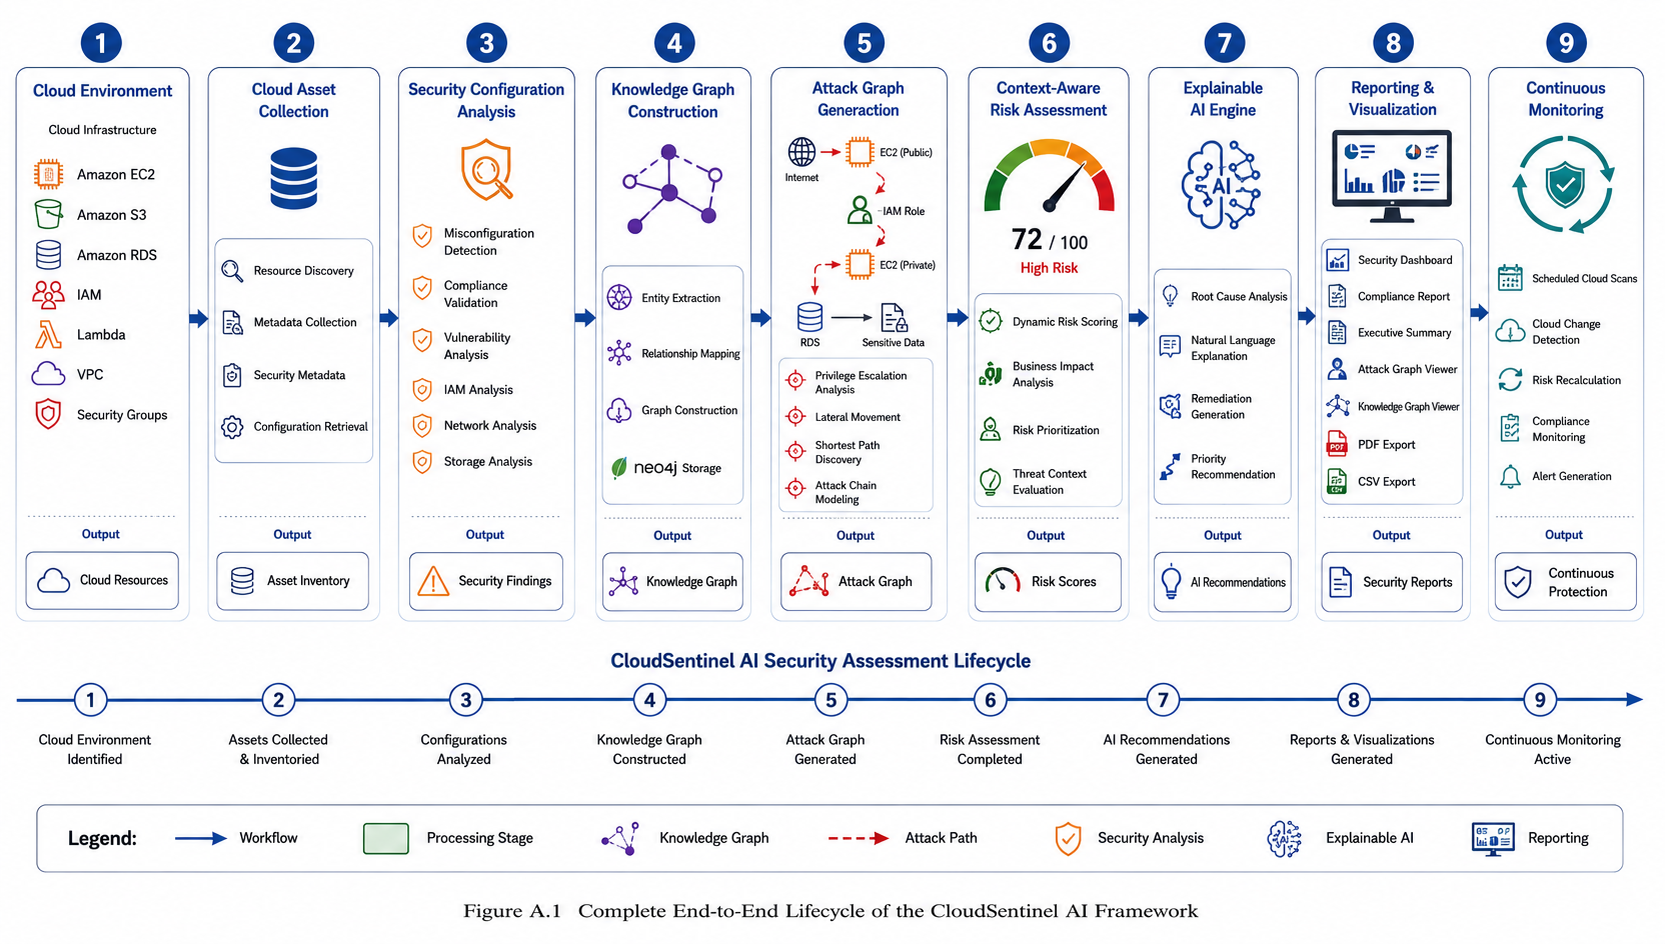
\includegraphics[width=0.9\textwidth,height=\textheight]{figures/image-a.1.png}
\caption{Appendix figure A.1.}\label{fig:a_1}
}
\end{figure}

\begin{figure}
\hypertarget{fig:a_2}{%
\centering
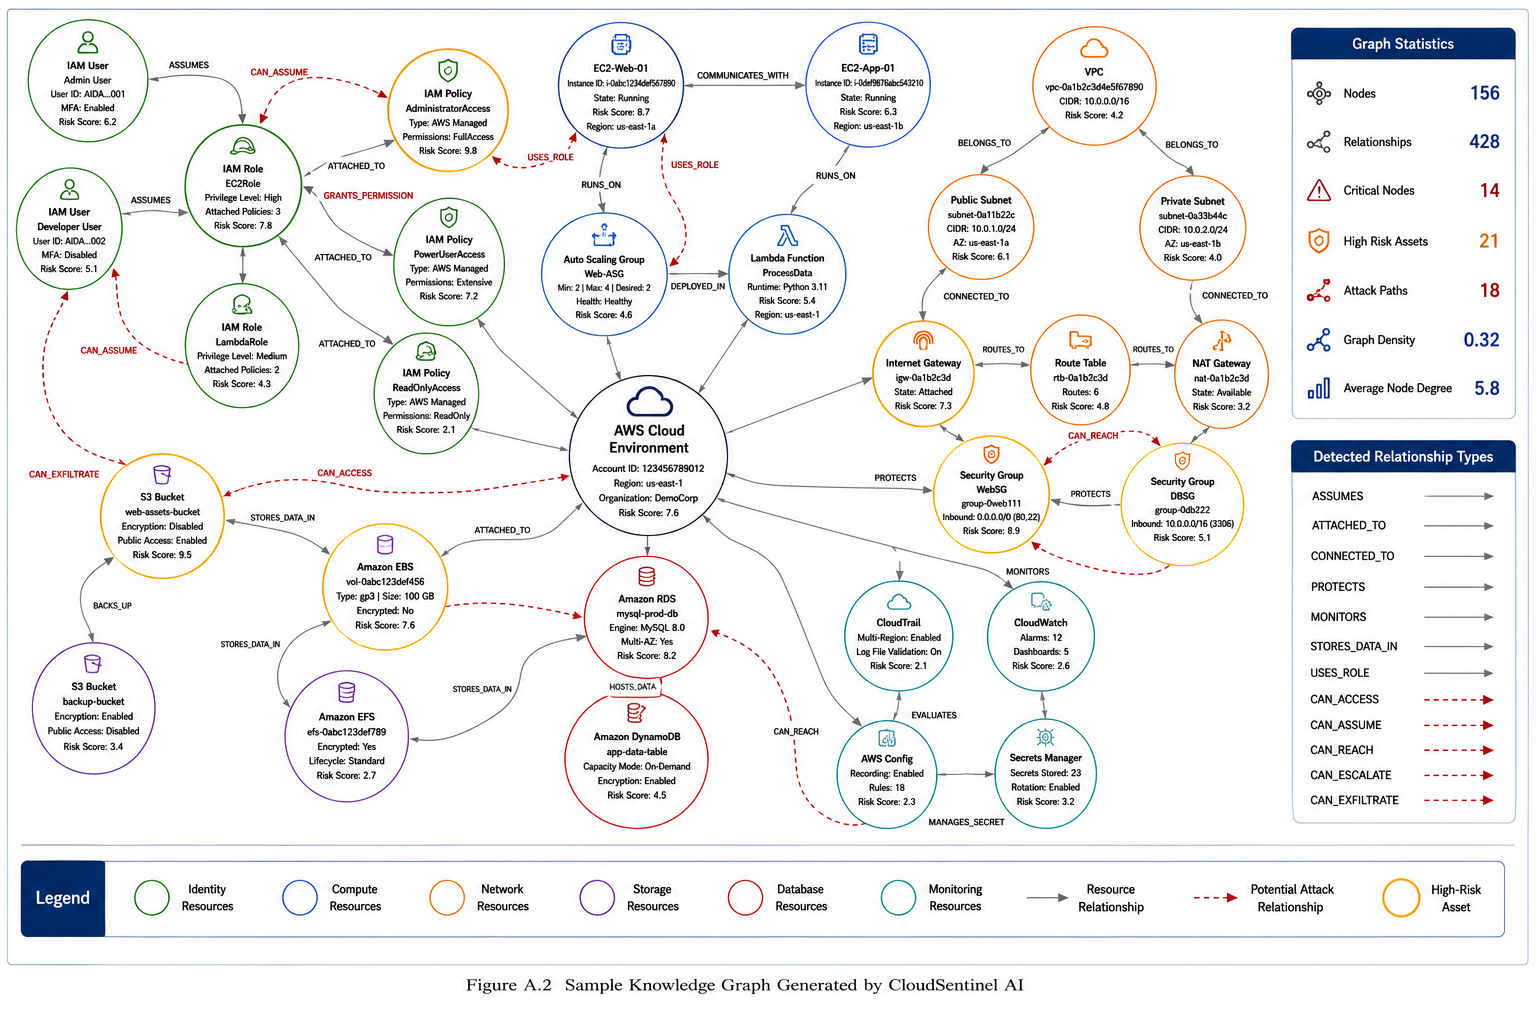
\includegraphics[width=0.9\textwidth,height=\textheight]{figures/image-a.2.png}
\caption{Appendix figure A.2.}\label{fig:a_2}
}
\end{figure}

\begin{figure}
\hypertarget{fig:a_3}{%
\centering
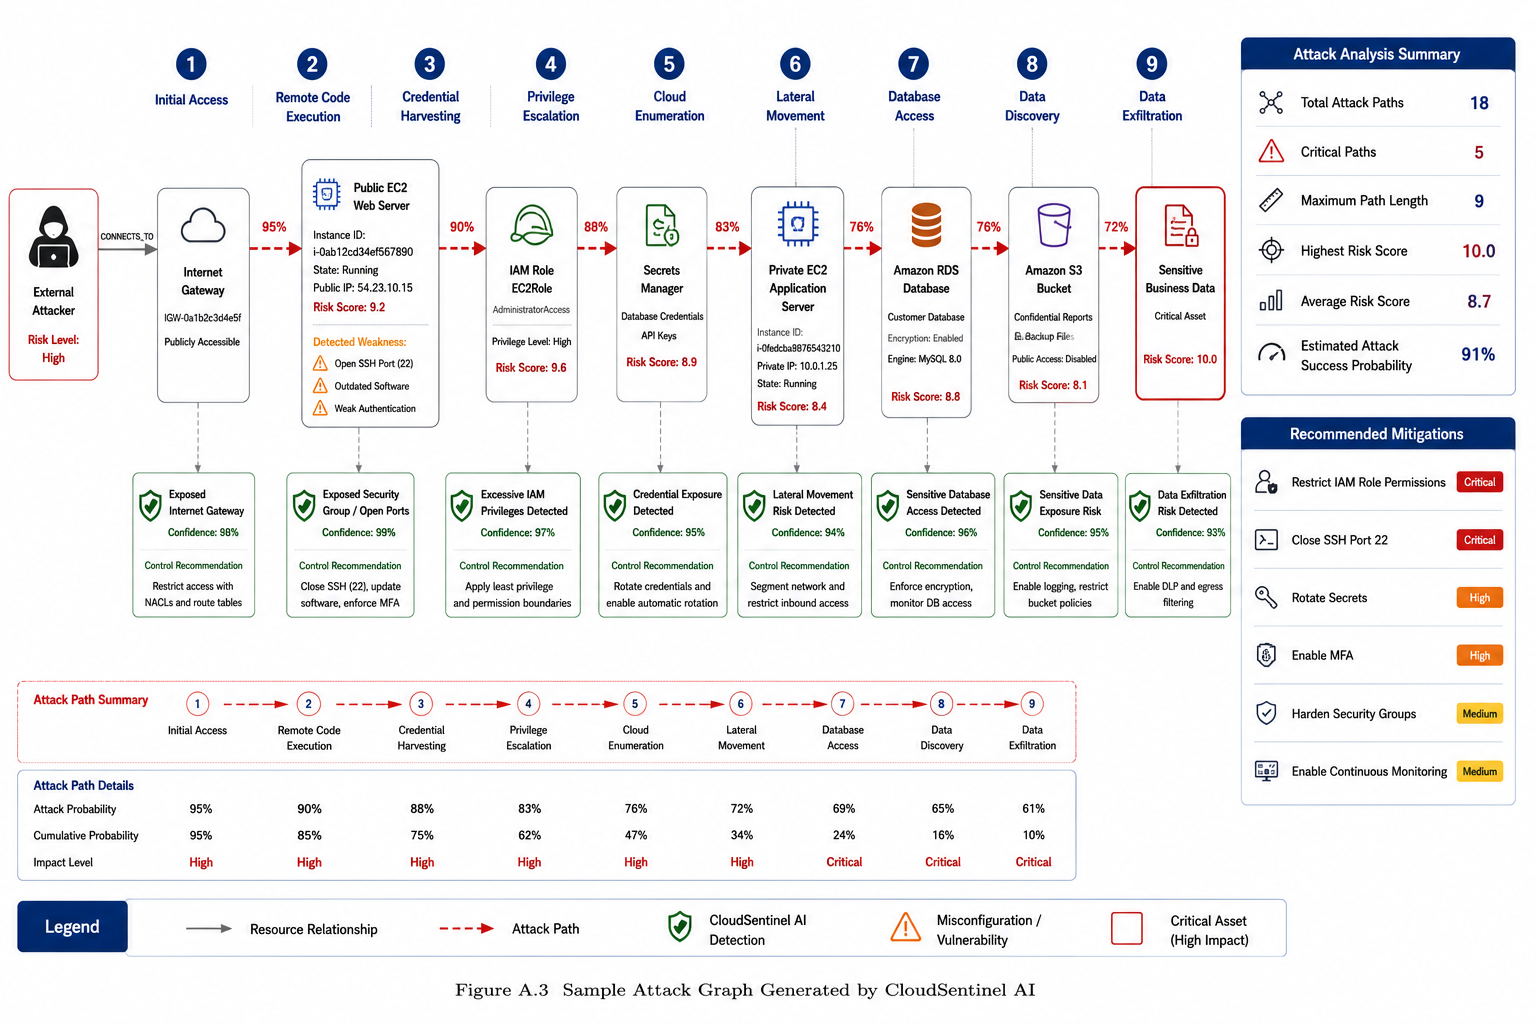
\includegraphics[width=0.9\textwidth,height=\textheight]{figures/image-a.3.png}
\caption{Appendix figure A.3.}\label{fig:a_3}
}
\end{figure}

\begin{figure}
\hypertarget{fig:a_4}{%
\centering
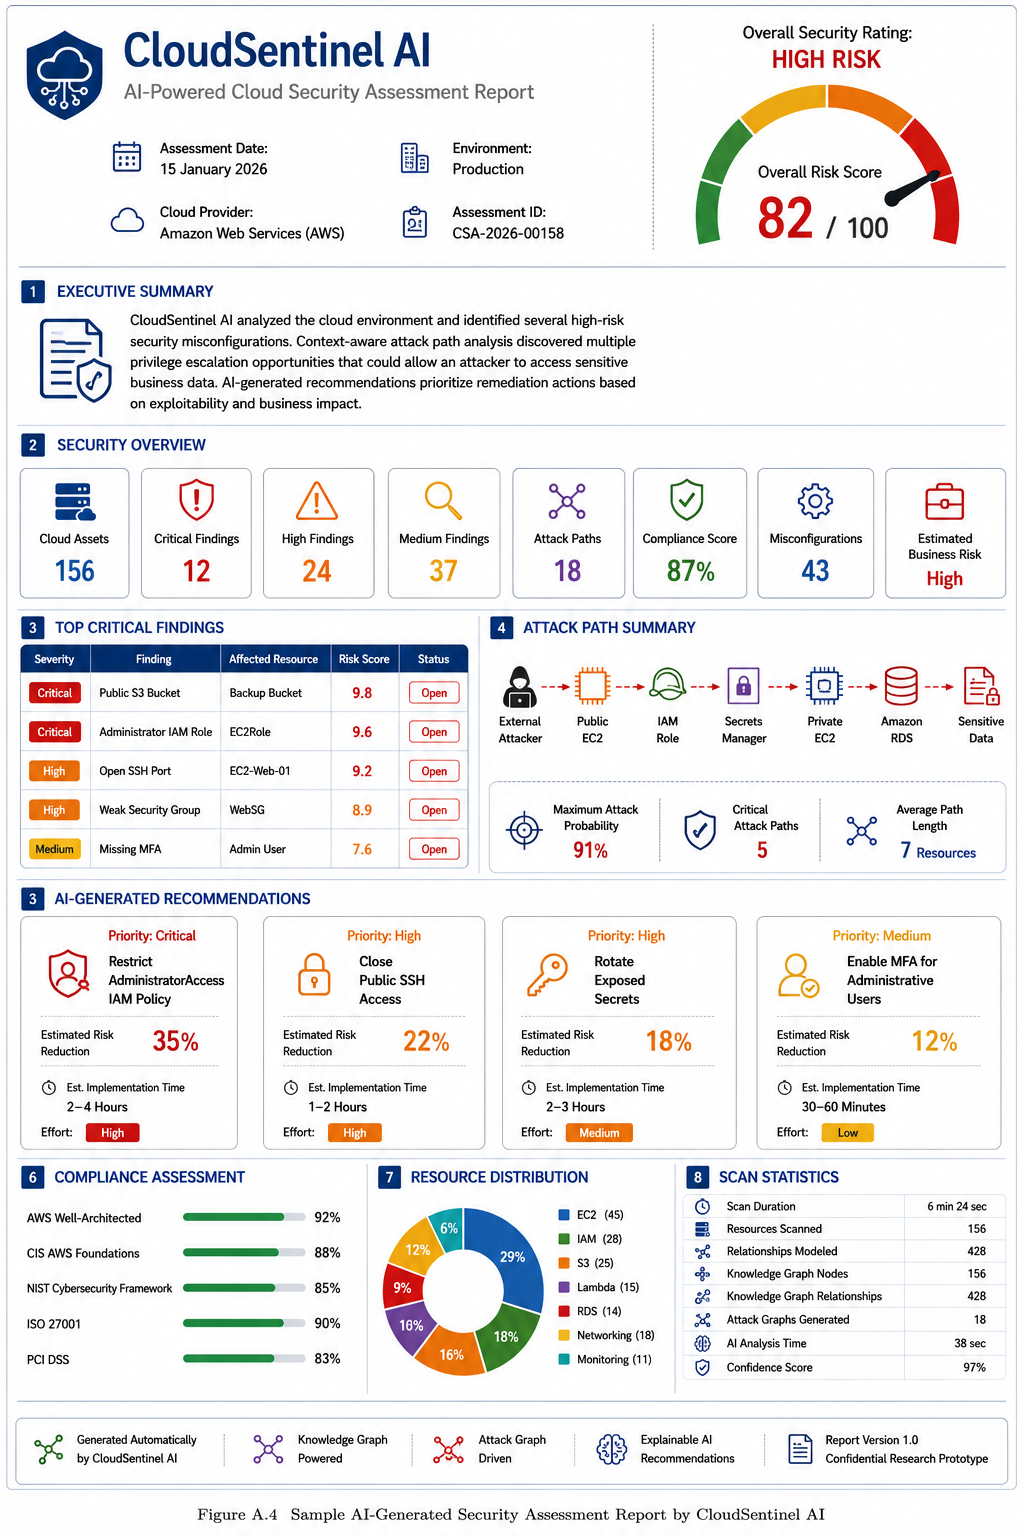
\includegraphics[width=0.9\textwidth,height=\textheight]{figures/image-a.4.png}
\caption{Appendix figure A.4.}\label{fig:a_4}
}
\end{figure}

\begin{figure}
\hypertarget{fig:a_5}{%
\centering
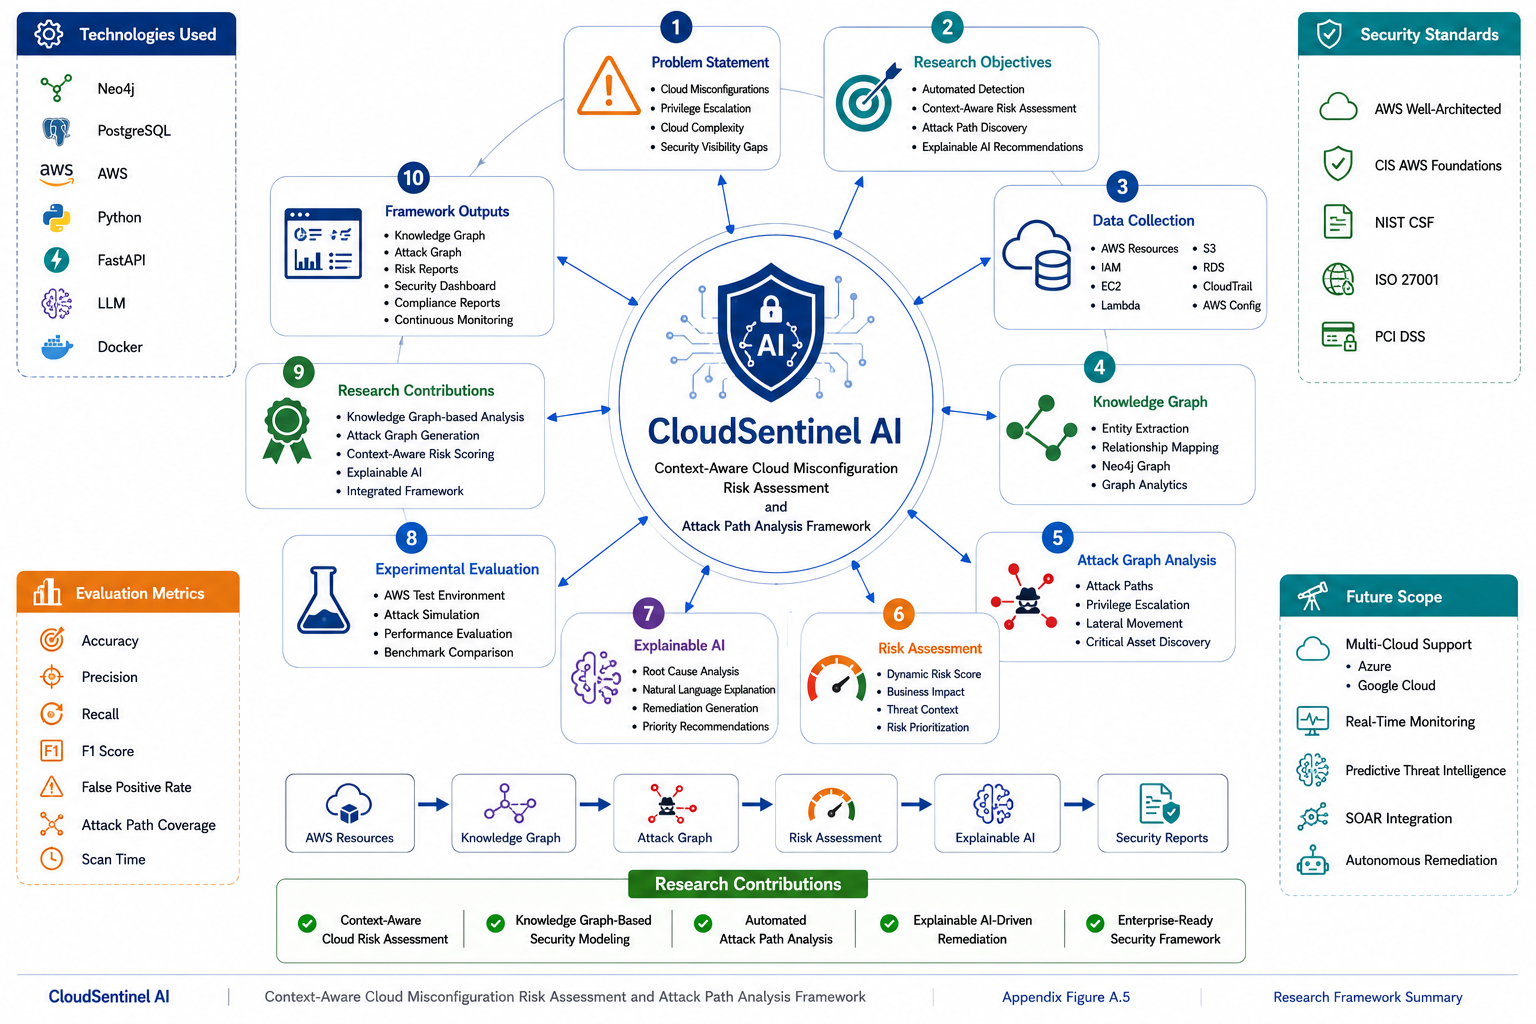
\includegraphics[width=0.9\textwidth,height=\textheight]{figures/image-a.5.png}
\caption{Appendix figure A.5.}\label{fig:a_5}
}
\end{figure}

\bibliographystyle{IEEEtran}
\bibliography{references}
\end{document}
